\documentclass[10pt,]{krantz}
\usepackage{lmodern}
\usepackage{amssymb,amsmath}
\usepackage{ifxetex,ifluatex}
\usepackage{fixltx2e} % provides \textsubscript
\ifnum 0\ifxetex 1\fi\ifluatex 1\fi=0 % if pdftex
  \usepackage[T1]{fontenc}
  \usepackage[utf8]{inputenc}
\else % if luatex or xelatex
  \ifxetex
    \usepackage{mathspec}
  \else
    \usepackage{fontspec}
  \fi
  \defaultfontfeatures{Ligatures=TeX,Scale=MatchLowercase}
\fi
% use upquote if available, for straight quotes in verbatim environments
\IfFileExists{upquote.sty}{\usepackage{upquote}}{}
% use microtype if available
\IfFileExists{microtype.sty}{%
\usepackage{microtype}
\UseMicrotypeSet[protrusion]{basicmath} % disable protrusion for tt fonts
}{}
\usepackage[unicode=true]{hyperref}
\PassOptionsToPackage{usenames,dvipsnames}{color} % color is loaded by hyperref
\hypersetup{
            pdftitle={Manual de R},
            colorlinks=true,
            linkcolor=Maroon,
            citecolor=Blue,
            urlcolor=Blue,
            breaklinks=true}
\urlstyle{same}  % don't use monospace font for urls
\usepackage{natbib}
\bibliographystyle{apalike}
\usepackage{color}
\usepackage{fancyvrb}
\newcommand{\VerbBar}{|}
\newcommand{\VERB}{\Verb[commandchars=\\\{\}]}
\DefineVerbatimEnvironment{Highlighting}{Verbatim}{commandchars=\\\{\}}
% Add ',fontsize=\small' for more characters per line
\usepackage{framed}
\definecolor{shadecolor}{RGB}{248,248,248}
\newenvironment{Shaded}{\begin{snugshade}}{\end{snugshade}}
\newcommand{\KeywordTok}[1]{\textcolor[rgb]{0.13,0.29,0.53}{\textbf{{#1}}}}
\newcommand{\DataTypeTok}[1]{\textcolor[rgb]{0.13,0.29,0.53}{{#1}}}
\newcommand{\DecValTok}[1]{\textcolor[rgb]{0.00,0.00,0.81}{{#1}}}
\newcommand{\BaseNTok}[1]{\textcolor[rgb]{0.00,0.00,0.81}{{#1}}}
\newcommand{\FloatTok}[1]{\textcolor[rgb]{0.00,0.00,0.81}{{#1}}}
\newcommand{\ConstantTok}[1]{\textcolor[rgb]{0.00,0.00,0.00}{{#1}}}
\newcommand{\CharTok}[1]{\textcolor[rgb]{0.31,0.60,0.02}{{#1}}}
\newcommand{\SpecialCharTok}[1]{\textcolor[rgb]{0.00,0.00,0.00}{{#1}}}
\newcommand{\StringTok}[1]{\textcolor[rgb]{0.31,0.60,0.02}{{#1}}}
\newcommand{\VerbatimStringTok}[1]{\textcolor[rgb]{0.31,0.60,0.02}{{#1}}}
\newcommand{\SpecialStringTok}[1]{\textcolor[rgb]{0.31,0.60,0.02}{{#1}}}
\newcommand{\ImportTok}[1]{{#1}}
\newcommand{\CommentTok}[1]{\textcolor[rgb]{0.56,0.35,0.01}{\textit{{#1}}}}
\newcommand{\DocumentationTok}[1]{\textcolor[rgb]{0.56,0.35,0.01}{\textbf{\textit{{#1}}}}}
\newcommand{\AnnotationTok}[1]{\textcolor[rgb]{0.56,0.35,0.01}{\textbf{\textit{{#1}}}}}
\newcommand{\CommentVarTok}[1]{\textcolor[rgb]{0.56,0.35,0.01}{\textbf{\textit{{#1}}}}}
\newcommand{\OtherTok}[1]{\textcolor[rgb]{0.56,0.35,0.01}{{#1}}}
\newcommand{\FunctionTok}[1]{\textcolor[rgb]{0.00,0.00,0.00}{{#1}}}
\newcommand{\VariableTok}[1]{\textcolor[rgb]{0.00,0.00,0.00}{{#1}}}
\newcommand{\ControlFlowTok}[1]{\textcolor[rgb]{0.13,0.29,0.53}{\textbf{{#1}}}}
\newcommand{\OperatorTok}[1]{\textcolor[rgb]{0.81,0.36,0.00}{\textbf{{#1}}}}
\newcommand{\BuiltInTok}[1]{{#1}}
\newcommand{\ExtensionTok}[1]{{#1}}
\newcommand{\PreprocessorTok}[1]{\textcolor[rgb]{0.56,0.35,0.01}{\textit{{#1}}}}
\newcommand{\AttributeTok}[1]{\textcolor[rgb]{0.77,0.63,0.00}{{#1}}}
\newcommand{\RegionMarkerTok}[1]{{#1}}
\newcommand{\InformationTok}[1]{\textcolor[rgb]{0.56,0.35,0.01}{\textbf{\textit{{#1}}}}}
\newcommand{\WarningTok}[1]{\textcolor[rgb]{0.56,0.35,0.01}{\textbf{\textit{{#1}}}}}
\newcommand{\AlertTok}[1]{\textcolor[rgb]{0.94,0.16,0.16}{{#1}}}
\newcommand{\ErrorTok}[1]{\textcolor[rgb]{0.64,0.00,0.00}{\textbf{{#1}}}}
\newcommand{\NormalTok}[1]{{#1}}
\usepackage{longtable,booktabs}
\usepackage{graphicx,grffile}
\makeatletter
\def\maxwidth{\ifdim\Gin@nat@width>\linewidth\linewidth\else\Gin@nat@width\fi}
\def\maxheight{\ifdim\Gin@nat@height>\textheight\textheight\else\Gin@nat@height\fi}
\makeatother
% Scale images if necessary, so that they will not overflow the page
% margins by default, and it is still possible to overwrite the defaults
% using explicit options in \includegraphics[width, height, ...]{}
\setkeys{Gin}{width=\maxwidth,height=\maxheight,keepaspectratio}
\IfFileExists{parskip.sty}{%
\usepackage{parskip}
}{% else
\setlength{\parindent}{0pt}
\setlength{\parskip}{6pt plus 2pt minus 1pt}
}
\setlength{\emergencystretch}{3em}  % prevent overfull lines
\providecommand{\tightlist}{%
  \setlength{\itemsep}{0pt}\setlength{\parskip}{0pt}}
\setcounter{secnumdepth}{5}
% Redefines (sub)paragraphs to behave more like sections
\ifx\paragraph\undefined\else
\let\oldparagraph\paragraph
\renewcommand{\paragraph}[1]{\oldparagraph{#1}\mbox{}}
\fi
\ifx\subparagraph\undefined\else
\let\oldsubparagraph\subparagraph
\renewcommand{\subparagraph}[1]{\oldsubparagraph{#1}\mbox{}}
\fi
\usepackage{booktabs}
\usepackage[spanish]{babel}
\decimalpoint
\selectlanguage{spanish}

% Comandos para escribir nombres de paquetes, programas y codigos
\newcommand{\pkg}[1]{{\normalfont\fontseries{b}\selectfont #1}}
\let\proglang=\textsf
\let\code=\texttt


\usepackage{booktabs}
\usepackage{longtable}
\usepackage[bf,singlelinecheck=off]{caption}

\usepackage{framed,color}
\definecolor{shadecolor}{RGB}{248,248,248}

\renewcommand{\textfraction}{0.05}
\renewcommand{\topfraction}{0.8}
\renewcommand{\bottomfraction}{0.8}
\renewcommand{\floatpagefraction}{0.75}

\renewenvironment{quote}{\begin{VF}}{\end{VF}}
\let\oldhref\href
\renewcommand{\href}[2]{#2\footnote{\url{#1}}}

\ifxetex
  \usepackage{letltxmacro}
  \setlength{\XeTeXLinkMargin}{1pt}
  \LetLtxMacro\SavedIncludeGraphics\includegraphics
  \def\includegraphics#1#{% #1 catches optional stuff (star/opt. arg.)
    \IncludeGraphicsAux{#1}%
  }%
  \newcommand*{\IncludeGraphicsAux}[2]{%
    \XeTeXLinkBox{%
      \SavedIncludeGraphics#1{#2}%
    }%
  }%
\fi

\makeatletter
\newenvironment{kframe}{%
\medskip{}
\setlength{\fboxsep}{.8em}
 \def\at@end@of@kframe{}%
 \ifinner\ifhmode%
  \def\at@end@of@kframe{\end{minipage}}%
  \begin{minipage}{\columnwidth}%
 \fi\fi%
 \def\FrameCommand##1{\hskip\@totalleftmargin \hskip-\fboxsep
 \colorbox{shadecolor}{##1}\hskip-\fboxsep
     % There is no \\@totalrightmargin, so:
     \hskip-\linewidth \hskip-\@totalleftmargin \hskip\columnwidth}%
 \MakeFramed {\advance\hsize-\width
   \@totalleftmargin\z@ \linewidth\hsize
   \@setminipage}}%
 {\par\unskip\endMakeFramed%
 \at@end@of@kframe}
\makeatother

\renewenvironment{Shaded}{\begin{kframe}}{\end{kframe}}

%%%%%

\newenvironment{rmdblock}[1]
  {
  \begin{itemize}
  \renewcommand{\labelitemi}{
    \raisebox{-.7\height}[0pt][0pt]{
      {\setkeys{Gin}{width=3em,keepaspectratio}\includegraphics{images/#1}}
    }
  }
  \setlength{\fboxsep}{1em}
  \begin{kframe}
  \item
  }
  {
  \end{kframe}
  \end{itemize}
  }
\newenvironment{rmdnote}
  {\begin{rmdblock}{note}}
  {\end{rmdblock}}
\newenvironment{rmdcaution}
  {\begin{rmdblock}{caution}}
  {\end{rmdblock}}
\newenvironment{rmdimportant}
  {\begin{rmdblock}{important}}
  {\end{rmdblock}}
\newenvironment{rmdtip}
  {\begin{rmdblock}{tip}}
  {\end{rmdblock}}
\newenvironment{rmdwarning}
  {\begin{rmdblock}{warning}}
  {\end{rmdblock}}


%%%%%


\usepackage{makeidx}
\makeindex

\urlstyle{tt}

\usepackage{amsthm}
\makeatletter
\def\thm@space@setup{%
  \thm@preskip=8pt plus 2pt minus 4pt
  \thm@postskip=\thm@preskip
}
\makeatother

\frontmatter

\title{Manual de R}
\author{Freddy Hernández Barajas\\
Olga Cecilia Usuga Manco}
\date{2017-02-26}

\let\BeginKnitrBlock\begin \let\EndKnitrBlock\end
\begin{document}
\maketitle

% you may need to leave a few empty pages before the dedication page

%\cleardoublepage\newpage\thispagestyle{empty}\null
%\cleardoublepage\newpage\thispagestyle{empty}\null
%\cleardoublepage\newpage
\thispagestyle{empty}

\begin{center}

Gracias a Dios por todo lo que me ha dado.

%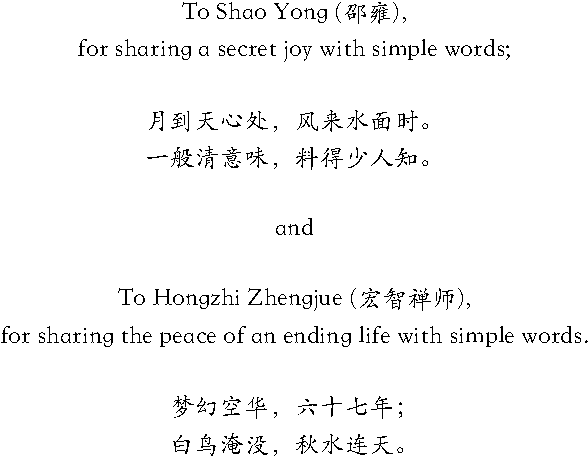
\includegraphics{images/dedication.pdf}
\end{center}

\setlength{\abovedisplayskip}{-5pt}
\setlength{\abovedisplayshortskip}{-5pt}

{
\hypersetup{linkcolor=black}
\setcounter{tocdepth}{2}
\tableofcontents
}
\listoftables
\listoffigures
\chapter*{Prefacio}\label{prefacio}


Este libro fue creado con la intención de apoyar el aprendizaje del
lenguaje de programación \proglang{R} en estudiantes de pregrado,
especialización, maestría e investigadores, que necesiten realizar
análisis estadísticos. En este libro se explica de una forma sencilla la
utilidad de la principales funciones para realizar diversos análisis
estadísticos, las cuestiones sobre creación de gráficos estadísticos no
son abordadas en el presente libro, recomendamos consultar
\citet{correa_hernandez}.

\section*{Estructura del libro}\label{estructura-del-libro}


El libro está estructurado de la siguiente manera.

En el capítulo \ref{central} se muestra como obtener las diversas
medidas de tendencial central para variables cuantitativas, el capítulo
\ref{varia} muestra como calcular las medidas de variabilidad, en el
capítulo \ref{posi} se ilustra cómo usar las funciones para obtener
medidas de posición y en el capítulo \ref{correl} se muestra como
obtener medidas de correlación entre pares de variables.

\section*{Información del software y
convenciones}\label{informacion-del-software-y-convenciones}


Para realizar este libro se usaron los paquetes de \proglang{R}
\textbf{knitr}\index{knitr} \citep{xie2015} y
\textbf{bookdown}\index{bookdown} \citep{R-bookdown}, estos paquetes
permiten construir todo el libro desde \proglang{R} y sirven para
incluir código que se ejecute de forma automática incluyendo las salidas
y gráficos.

En todo el libro se presentarán códigos que el lector puede copiar y
pegar en su consola de \proglang{R} para obtener los mismos resultados
aquí presentados. Los códigos se destacan en una caja de color beis (o
beige) similar a la mostrada a continuación.

\begin{Shaded}
\begin{Highlighting}[]
\DecValTok{4} \NormalTok{+}\StringTok{ }\DecValTok{6}
\NormalTok{a <-}\StringTok{ }\KeywordTok{c}\NormalTok{(}\DecValTok{1}\NormalTok{, }\DecValTok{5}\NormalTok{, }\DecValTok{6}\NormalTok{)}
\DecValTok{5} \NormalTok{*}\StringTok{ }\NormalTok{a}
\DecValTok{1}\NormalTok{:}\DecValTok{10}
\end{Highlighting}
\end{Shaded}

Los resultados o salidas obtenidos de cualquier código se destacan con
dos símbolos de númeral (\texttt{\#\#}) al inicio de cada línea o
renglón, esto quiere decir que todo lo que inicie con \texttt{\#\#} son
resultados obtenidos y el usuario \textbf{NO} los debe copiar. Abajo se
muestran los resultados obtenidos luego de correr el código anterior.

\begin{verbatim}
## [1] 10
\end{verbatim}

\begin{verbatim}
## [1]  5 25 30
\end{verbatim}

\begin{verbatim}
##  [1]  1  2  3  4  5  6  7  8  9 10
\end{verbatim}

\section*{Bloques informativos}\label{bloques-informativos}


En varias partes del libro usaremos bloques informativos para resaltar
algún aspecto importante. Abajo se encuentra un ejemplo de los bloques y
su significado.

\BeginKnitrBlock{rmdnote}
Nota aclaratoria.
\EndKnitrBlock{rmdnote}

\BeginKnitrBlock{rmdtip}
Sugerencia.
\EndKnitrBlock{rmdtip}

\BeginKnitrBlock{rmdwarning}
Advertencia.
\EndKnitrBlock{rmdwarning}

\section*{Agradecimientos}\label{agradecimientos}


Agradecemos enormemente a todos los estudiantes, profesores e
investigadores que han leído este libro y nos han retroalimentado con
comentarios valiosos para mejorar el documento.

\BeginKnitrBlock{flushright}
Freddy Hernández Barajas

Olga Cecilia Usuga Manco
\EndKnitrBlock{flushright}

\chapter*{Sobre los autores}\label{sobre-los-autores}


Freddy Hernández Barajas es profesor asistente de la Universidad
Nacional de Colombia adscrito a la Escuela de Estadística de la Facultad
de Ciencias.

Olga Cecilia Usuga Manco es profesora asociada de la Universidad de
Antioquia adscrita al Departamento de Ingeniería Industrial de la
Facultad de Ingeniería.

\mainmatter

\chapter{Introducción}\label{introduccion}

\section{Orígenes} \label{sec:origenes}

\proglang{R} es un lenguaje de programación usado para realizar
procedimientos estadísticos y gráficos de alto nivel, este lenguaje fue
creado en 1993 por los profesores e investigadores Robert Gentleman y
Ross Ihaka. Inicialmente el lenguaje se usó para apoyar los cursos que
tenían a su cargo los profesores, pero luego de ver la utilidad de la
herramienta desarrollada, decidieron colocar copias de \proglang{R} en
StatLib. A partir de 1995 el código fuente de \proglang{R} está
disponible bajo licencia GNU GPL para sistemas operativos Windows,
Macintosh y distribuciones Unix/Linux. La comunidad de usuarios de
\proglang{R} en el mundo es muy grande y los usuarios cuentan con
diferentes espacios para interactuar, a continuación una lista no
exhaustiva de los sitios más populares relacionados con \proglang{R}:

\begin{itemize}
\tightlist
\item
  \href{https://www.r-bloggers.com/}{Rbloggers}.
\item
  \href{http://r-es.org/}{Comunidad hispana de \proglang{R}}.
\item
  \href{http://r.789695.n4.nabble.com/}{Nabble}.
\item
  \href{http://r-br.2285057.n4.nabble.com/}{Foro en portugués}.
\item
  \href{http://stackoverflow.com/questions/tagged/r}{Stackoverflow}.
\item
  \href{http://stats.stackexchange.com/questions/tagged/r}{Cross
  Validated}.
\item
  \href{https://stat.ethz.ch/mailman/listinfo/r-help}{\proglang{R}-Help
  Mailing List}.
\item
  \href{http://blog.revolutionanalytics.com/}{Revolutions}.
\item
  \href{https://www.r-statistics.com/}{\proglang{R}-statistics blog}.
\item
  \href{https://rdatamining.wordpress.com/}{RDataMining}.
\end{itemize}

\begin{figure}

{\centering 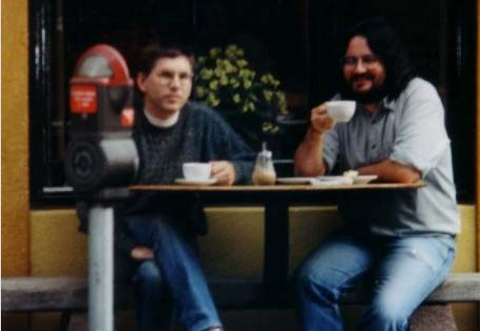
\includegraphics{images/Robert_Roos} 

}

\caption{Robert Gentleman (izquierda) y Ross Ihaka (derecha) creadores de R.}\label{fig:unnamed-chunk-7}
\end{figure}

\section{Descarga e instalación} \label{sec:descarga}

Para realizar la instalación de \proglang{R} usted debe visitar la
página del CRAN (\textit{Comprehensive R Archive Network}) disponible en
este \href{https://cran.r-project.org/}{enlace}. Una vez ingrese a la
página encontrará un cuadro similar al mostrado en la Figura
\ref{fig:cran} donde aparecen los enlaces de la instalación para los
sistemas operativos Linux, Mac y Windows.

\begin{figure}

{\centering 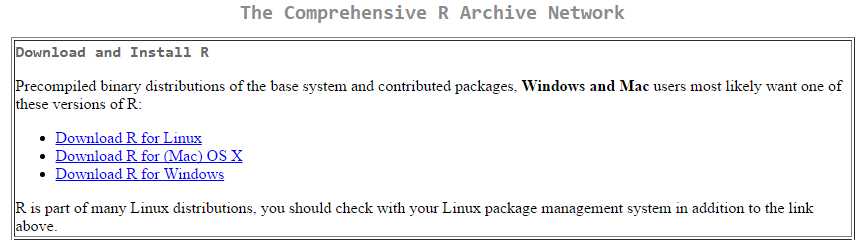
\includegraphics{images/cran} 

}

\caption{Página del Cran.}\label{fig:cran}
\end{figure}

Supongamos que se desea instalar \proglang{R} en Windows, para esto se
debe dar clic sobre el hiperenlace
\textcolor{BurntOrange}{Download R for Windows} de la Figura
\ref{fig:cran}. Una vez hecho esto se abrirá una página con el contenido
mostrado en la Figura \ref{fig:inst1}. Una vez ingrese a esa nueva
página usted debe dar clic sobre el hiperenlace
\textcolor{BurntOrange}{install R for the first time} como es señalado
por la flecha roja en la Figura \ref{fig:inst1}.

\begin{figure}

{\centering 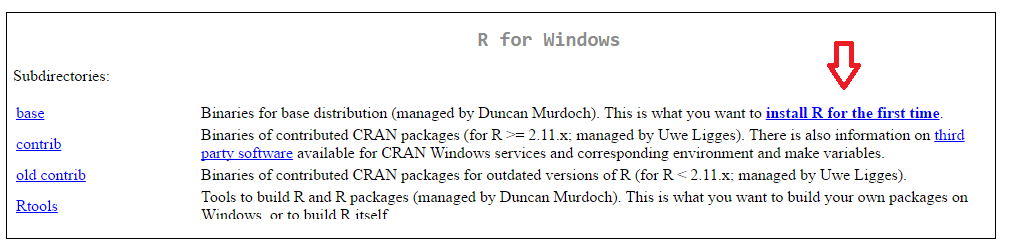
\includegraphics{images/instalacion1} 

}

\caption{Página de instalación para la primera ocasión.}\label{fig:inst1}
\end{figure}

Luego de esto se abrirá otra página con un encabezado similar al
mostrado en la Figura \ref{fig:inst2}, al momento de capturar la figura
la versión actual de \proglang{R} era 3.2.5 pero seguramente en este
momento usted tendrá disponible una versión actualizada. Una vez allí
uste debe dar clic sobre
\textcolor{BurntOrange}{Download R 3.2.5 for Windows} como es señalado
por la flecha verde. Luego de esto se descargará el instalador
\proglang{R} en el computador el cual deberá ser instalado con las
opciones que vienen por defecto.

\begin{figure}

{\centering 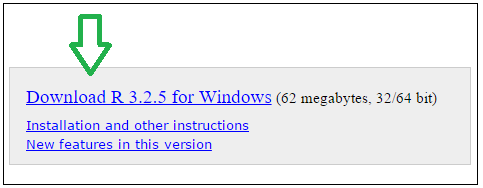
\includegraphics{images/instalacion2} 

}

\caption{Página de descarga.}\label{fig:inst2}
\end{figure}

Se recomienda observar el siguiente video didáctico de instalación de
\proglang{R} disponible en este
\href{http://tinyurl.com/jd7b9ks}{enlace} para facilitar la tarea de
instalación.

\section{Apariencia del programa} \label{sec:apariencia}

Una vez que esté instalado \proglang{R} en su computador, usted podrá
acceder a él por la lista de programas o por medio del acceso directo
que quedó en el escritorio, en la Figura \ref{fig:rlogo} se muestra la
apariencia del acceso directo para ingresar a \proglang{R}.

\begin{figure}

{\centering 
\includegraphics{images/rlogo} 

}

\caption{Apariencia del acceso directo para ingresar a R.}\label{fig:rlogo}
\end{figure}

Al abrir \proglang{R} aparecerá en la pantalla de su computador algo
similar a lo que está en la Figura \ref{fig:pantalla}. La ventana
izquierda se llama consola y es donde se ingresan las instrucciones, una
vez que se construye un gráfico se activa otra ventana llamada ventana
gráfica. Cualquier usuario puede modificar la posición y tamaños de
estas ventanas, puede cambiar el tipo y tamaño de las letras en la
consola, para hacer esto se deben explorar las opciones de
\textit{editar} en la barra de herramientas.

\begin{figure}

{\centering 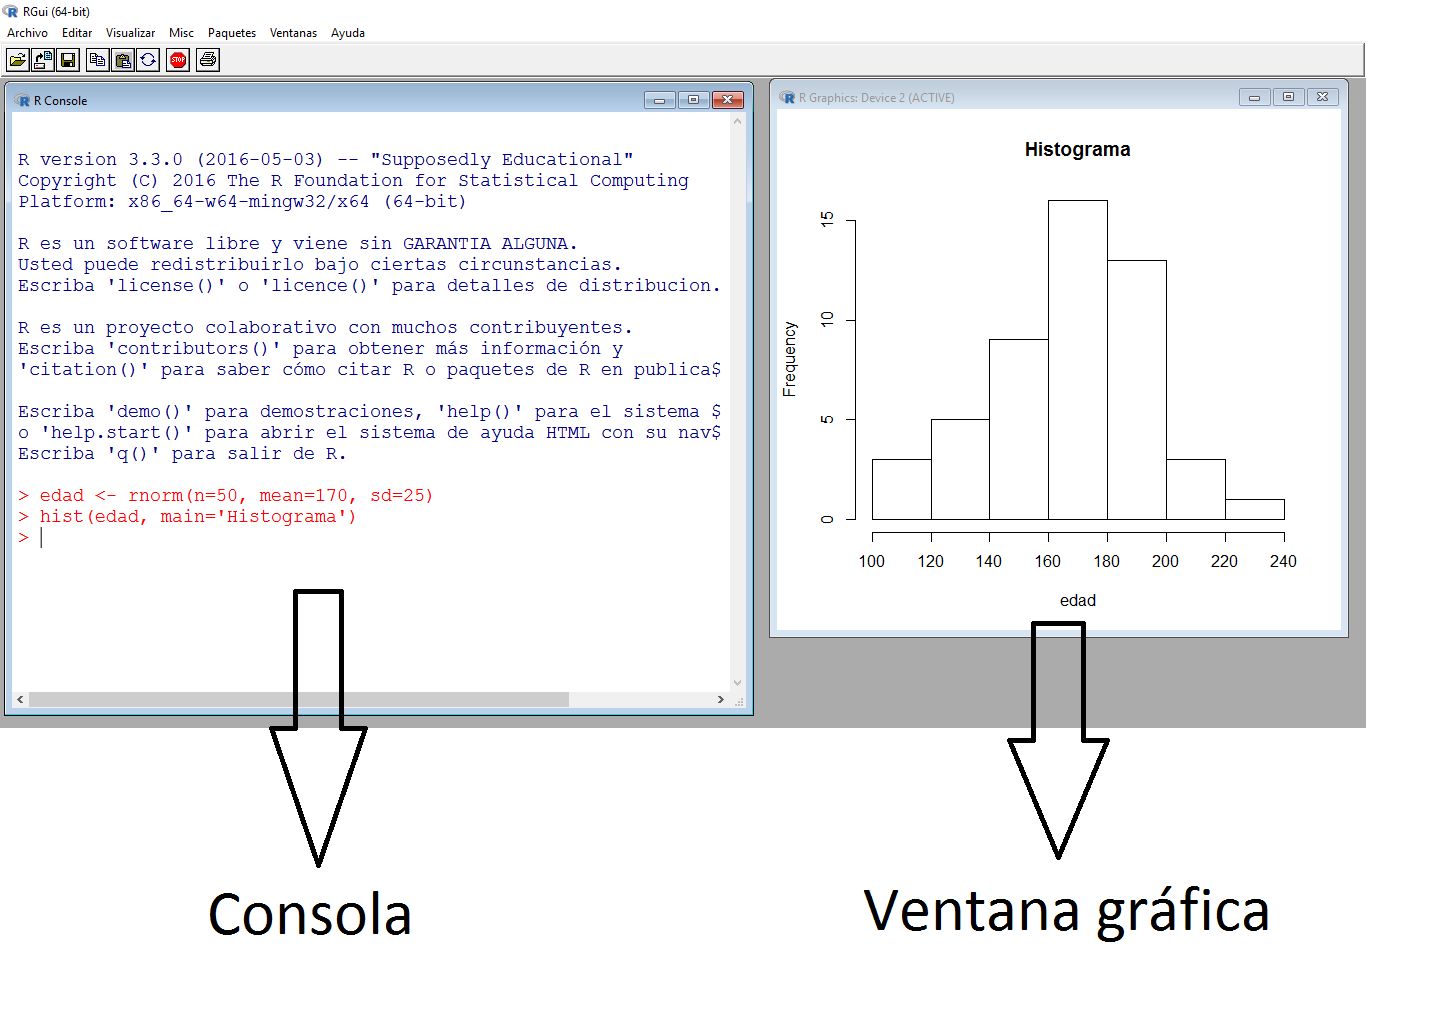
\includegraphics{images/Rpantallazo} 

}

\caption{Apariencia de R.}\label{fig:pantalla}
\end{figure}

\chapter{\texorpdfstring{Tipos de objetos \index{objetos}
\label{objetos}}{Tipos de objetos  }}\label{tipos-de-objetos}

En \proglang{R} existen varios tipos de objectos que permiten que el
usuario pueda almacenar la información para realizar procedimientos
estadísticos y gráficos. Los principales objetos en \proglang{R} son
vectores, matrices, arreglos, marcos de datos y listas. A continuación
se presentan las características de estos objetos y la forma para
crearlos.

\section{\texorpdfstring{Vectores \index{vector}
\label{vector}}{Vectores  }}\label{vectores}

Los vectores vectores son arreglos ordenados en los cuales se puede
almacenar información de tipo numérico (variable cuantitativa),
alfanumérico (variable cualitativa) o lógico (\texttt{TRUE} o
\texttt{FALSE}), pero no mezclas de éstos. La función de \proglang{R}
para crear un vector es \texttt{c()} y que significa concatenar; dentro
de los paréntesis de esta función se ubica la información a almacenar.
Una vez construído el vector se acostumbra a etiquetarlo con un nombre
corto y representativo de la información que almacena, la asignación se
hace por medio del operador \texttt{\textless{}-} entre el nombre y el
vector.

A continuación se presenta un ejemplo de cómo crear tres vectores que
contienen las respuestas de cinco personas a tres preguntas que se les
realizaron.

\begin{Shaded}
\begin{Highlighting}[]
\NormalTok{edad <-}\StringTok{ }\KeywordTok{c}\NormalTok{(}\DecValTok{15}\NormalTok{, }\DecValTok{19}\NormalTok{, }\DecValTok{13}\NormalTok{, }\OtherTok{NA}\NormalTok{, }\DecValTok{20}\NormalTok{)}
\NormalTok{deporte <-}\StringTok{ }\KeywordTok{c}\NormalTok{(}\OtherTok{TRUE}\NormalTok{, }\OtherTok{TRUE}\NormalTok{, }\OtherTok{NA}\NormalTok{, }\OtherTok{FALSE}\NormalTok{, }\OtherTok{TRUE}\NormalTok{)}
\NormalTok{comic.fav <-}\StringTok{ }\KeywordTok{c}\NormalTok{(}\OtherTok{NA}\NormalTok{, }\StringTok{'Superman'}\NormalTok{, }\StringTok{'Batman'}\NormalTok{, }\OtherTok{NA}\NormalTok{, }\StringTok{'Batman'}\NormalTok{)}
\end{Highlighting}
\end{Shaded}

El vector \texttt{edad} es un vector cuantitativo y contiene las edades
de las 5 personas. En la cuarta posición del vector se colocó el símbolo
\texttt{NA} que significa \textit{Not Available} debido a que no se
registró la edad para esa persona. Al hacer una asignación se acostumbra
a dejar un espacio antes y después del operador \texttt{\textless{}-} de
asignación. El segundo vector es llamado \texttt{deporte} y es un vector
lógico que almacena las respuestas a la pregunta de si la persona
practica deporte, nuevamente aquí hay un \texttt{NA} para la tercera
persona. El último vector \texttt{comic.fav} contiene la información del
cómic favorito de cada persona, como esta variable es cualitativa es
necesario usar las comillas
\texttt{\textquotesingle{}\ \textquotesingle{}} para encerrar las
respuestas.

\BeginKnitrBlock{rmdwarning}
Cuando se usa \texttt{NA} para representar una información
\textit{Not Available} no se deben usar comillas.
\EndKnitrBlock{rmdwarning}

\BeginKnitrBlock{rmdnote}
Es posible usar comillas sencillas
\texttt{\textquotesingle{}foo\textquotesingle{}} o comillas dobles
\texttt{"foo"} para ingresar valores de una variable cualitativa.
\EndKnitrBlock{rmdnote}

Si se desea ver lo que está almacenado en cada uno de estos vectores, se
debe escribir en la consola de \proglang{R} el nombre de uno de los
objetos y luego se presiona la tecla \textit{enter} o \textit{intro}, al
realizar esto lo que se obtiene se muestra a continuación.

\begin{Shaded}
\begin{Highlighting}[]
\NormalTok{edad}
\end{Highlighting}
\end{Shaded}

\begin{verbatim}
## [1] 15 19 13 NA 20
\end{verbatim}

\begin{Shaded}
\begin{Highlighting}[]
\NormalTok{deporte}
\end{Highlighting}
\end{Shaded}

\begin{verbatim}
## [1]  TRUE  TRUE    NA FALSE  TRUE
\end{verbatim}

\begin{Shaded}
\begin{Highlighting}[]
\NormalTok{comic.fav}
\end{Highlighting}
\end{Shaded}

\begin{verbatim}
## [1] NA         "Superman" "Batman"   NA        
## [5] "Batman"
\end{verbatim}

\subsection{¿Cómo extraer elementos de un
vector?}\label{como-extraer-elementos-de-un-vector}

Para extraer un elemento almacenado dentro un vector se usan los
corchetes \texttt{{[}{]}} y dentro de ellos la posición o posiciones que
interesan.

\subsection*{Ejemplo}\label{ejemplo}


Si queremos extraer la edad de la tercera persona escribimos el nombre
del vector y luego \texttt{{[}3{]}} para indicar la tercera posición de
\texttt{edad}, a continuación el código.

\begin{Shaded}
\begin{Highlighting}[]
\NormalTok{edad[}\DecValTok{3}\NormalTok{]}
\end{Highlighting}
\end{Shaded}

\begin{verbatim}
## [1] 13
\end{verbatim}

Si queremos conocer el cómic favorito de la segunda y quinta persona,
escribimos el nombre del vector y luego, dentro de los corchetes,
escribimos otro vector con las posiciones 2 y 5 que nos interesan así
\texttt{{[}c(2,\ 5){]}}, a continuación el código.

\begin{Shaded}
\begin{Highlighting}[]
\NormalTok{comic.fav[}\KeywordTok{c}\NormalTok{(}\DecValTok{2}\NormalTok{, }\DecValTok{5}\NormalTok{)]}
\end{Highlighting}
\end{Shaded}

\begin{verbatim}
## [1] "Superman" "Batman"
\end{verbatim}

Si nos interesan las respuestas de la práctica de deporte, excepto la de
la persona 3, usamos \texttt{{[}-3{]}} luego del nombre del vector para
obtener todo, excepto la tercera posición.

\begin{Shaded}
\begin{Highlighting}[]
\NormalTok{deporte[-}\DecValTok{3}\NormalTok{]}
\end{Highlighting}
\end{Shaded}

\begin{verbatim}
## [1]  TRUE  TRUE FALSE  TRUE
\end{verbatim}

\BeginKnitrBlock{rmdwarning}
Si desea extraer varios posiciones de un vector NUNCA escriba esto:
\texttt{mivector{[}2,\ 5,\ 7{]}}. Tiene que crear un vector con las
posiciones y luego colocarlo dentro de los corchetes así:
\texttt{mivector{[}c(2,\ 5,\ 7){]}}
\EndKnitrBlock{rmdwarning}

\section{Matrices}\label{matrices}

Las matrices \index{matrices} son arreglos rectangulares de filas y
columnas con información numérica, alfanumérica o lógica. Para construir
una matriz se usa la función \texttt{matrix(\ )}. Por ejemplo, para
crear una matriz de 4 filas y 5 columnas (de dimensión \(4 \times 5\))
con los primeros 20 números positivos se escribe el código siguiente en
la consola.

\begin{Shaded}
\begin{Highlighting}[]
\NormalTok{mimatriz <-}\StringTok{ }\KeywordTok{matrix}\NormalTok{(}\DataTypeTok{data=}\DecValTok{1}\NormalTok{:}\DecValTok{20}\NormalTok{, }\DataTypeTok{nrow=}\DecValTok{4}\NormalTok{, }\DataTypeTok{ncol=}\DecValTok{5}\NormalTok{, }\DataTypeTok{byrow=}\OtherTok{FALSE}\NormalTok{)}
\end{Highlighting}
\end{Shaded}

El argumento \texttt{data} de la función sirve para indicar los datos
que se van a almacenar en la matriz, los argumentos \texttt{nrow} y
\texttt{ncol} sirven para definir la dimensión de la matriz y por último
el argumento \texttt{byrow} sirve para indicar si la información
contenida en \texttt{data} se debe ingresar por filas o no. Para
observar lo que quedó almacenado en el objeto \texttt{mimatriz} se
escribe en la consola el nombre del objeto seguido de la tecla
\textit{enter} o \textit{intro}.

\begin{Shaded}
\begin{Highlighting}[]
\NormalTok{mimatriz}
\end{Highlighting}
\end{Shaded}

\begin{verbatim}
##      [,1] [,2] [,3] [,4] [,5]
## [1,]    1    5    9   13   17
## [2,]    2    6   10   14   18
## [3,]    3    7   11   15   19
## [4,]    4    8   12   16   20
\end{verbatim}

\subsection{¿Cómo extraer elementos de una
matriz?}\label{como-extraer-elementos-de-una-matriz}

Al igual que en el caso de los vectores, para extraer elementos
almacenados dentro de una matriz se usan los corchetes
\texttt{{[}\ ,\ {]}} y dentro, separado por una coma, el número de
fila(s) y el número de columna(s) que nos interesan.

\subsection*{Ejemplo}\label{ejemplo-1}


Si queremos extraer el valor almacenado en la fila 3 y columna 4 usamos
el siguiente código.

\begin{Shaded}
\begin{Highlighting}[]
\NormalTok{mimatriz[}\DecValTok{3}\NormalTok{, }\DecValTok{4}\NormalTok{]}
\end{Highlighting}
\end{Shaded}

\begin{verbatim}
## [1] 15
\end{verbatim}

Si queremos recuperar \textbf{toda} la fila 2 usamos el siguiente
código.

\begin{Shaded}
\begin{Highlighting}[]
\NormalTok{mimatriz[}\DecValTok{2}\NormalTok{, ]  }\CommentTok{# No se escribe nada luego de la coma}
\end{Highlighting}
\end{Shaded}

\begin{verbatim}
## [1]  2  6 10 14 18
\end{verbatim}

Si queremos recuperar \textbf{toda} la columna 5 usamos el siguiente
código.

\begin{Shaded}
\begin{Highlighting}[]
\NormalTok{mimatriz[, }\DecValTok{5}\NormalTok{]  }\CommentTok{# No se escribe nada antes de la coma}
\end{Highlighting}
\end{Shaded}

\begin{verbatim}
## [1] 17 18 19 20
\end{verbatim}

Si queremos recuperar la matriz original sin las columnas 2 y 4 usamos
el siguiente código.

\begin{Shaded}
\begin{Highlighting}[]
\NormalTok{mimatriz[, -}\KeywordTok{c}\NormalTok{(}\DecValTok{2}\NormalTok{, }\DecValTok{4}\NormalTok{)]  }\CommentTok{# Las columnas como vector}
\end{Highlighting}
\end{Shaded}

\begin{verbatim}
##      [,1] [,2] [,3]
## [1,]    1    9   17
## [2,]    2   10   18
## [3,]    3   11   19
## [4,]    4   12   20
\end{verbatim}

Si queremos recuperar la matriz original sin la fila 1 ni columna 3
usamos el siguiente código.

\begin{Shaded}
\begin{Highlighting}[]
\NormalTok{mimatriz[-}\DecValTok{1}\NormalTok{, -}\DecValTok{3}\NormalTok{]  }\CommentTok{# Signo de menos para eliminar}
\end{Highlighting}
\end{Shaded}

\begin{verbatim}
##      [,1] [,2] [,3] [,4]
## [1,]    2    6   14   18
## [2,]    3    7   15   19
## [3,]    4    8   16   20
\end{verbatim}

\section{\texorpdfstring{Arreglos \index{arreglo}
\index{array}}{Arreglos  }}\label{arreglos}

Un arreglo es una matriz de varias dimensiones con información numérica,
alfanumérica o lógica. Para construir una arreglo se usa la función
\texttt{array(\ )}. Por ejemplo, para crear un arreglo de
\(3 \times 4 \times 2\) con las primeras 24 letras minúsculas del
alfabeto se escribe el siguiente código.

\begin{Shaded}
\begin{Highlighting}[]
\NormalTok{miarray <-}\StringTok{ }\KeywordTok{array}\NormalTok{(}\DataTypeTok{data=}\NormalTok{letters[}\DecValTok{1}\NormalTok{:}\DecValTok{24}\NormalTok{], }\DataTypeTok{dim=}\KeywordTok{c}\NormalTok{(}\DecValTok{3}\NormalTok{, }\DecValTok{4}\NormalTok{, }\DecValTok{2}\NormalTok{))}
\end{Highlighting}
\end{Shaded}

El argumento \texttt{data} de la función sirve para indicar los datos
que se van a almacenar en el arreglo y el argumento \texttt{dim} sirve
para indicar las dimensiones del arreglo. Para observar lo que quedó
almacenado en el objeto \texttt{miarray} se escribe en la consola lo
siguiente.

\begin{Shaded}
\begin{Highlighting}[]
\NormalTok{miarray}
\end{Highlighting}
\end{Shaded}

\begin{verbatim}
## , , 1
## 
##      [,1] [,2] [,3] [,4]
## [1,] "a"  "d"  "g"  "j" 
## [2,] "b"  "e"  "h"  "k" 
## [3,] "c"  "f"  "i"  "l" 
## 
## , , 2
## 
##      [,1] [,2] [,3] [,4]
## [1,] "m"  "p"  "s"  "v" 
## [2,] "n"  "q"  "t"  "w" 
## [3,] "o"  "r"  "u"  "x"
\end{verbatim}

\subsection{¿Cómo extraer elementos de un
arreglo?}\label{como-extraer-elementos-de-un-arreglo}

Para recuperar elementos almacenados en un arreglo se usan también
corchetes, y dentro de los corchetes, las coordenadas del objeto de
interés.

\subsection*{Ejemplo}\label{ejemplo-2}


Si queremos extraer la letra almacenada en la fila 1 y columna 3 de la
segunda capa de \texttt{miarray} usamos el siguiente código.

\begin{Shaded}
\begin{Highlighting}[]
\NormalTok{miarray[}\DecValTok{1}\NormalTok{, }\DecValTok{3}\NormalTok{, }\DecValTok{2}\NormalTok{]  }\CommentTok{# El orden es importante}
\end{Highlighting}
\end{Shaded}

\begin{verbatim}
## [1] "s"
\end{verbatim}

Si queremos extraer la segunda capa completa usamos el siguiente código.

\begin{Shaded}
\begin{Highlighting}[]
\NormalTok{miarray[,, }\DecValTok{2}\NormalTok{]  }\CommentTok{# No se coloca nada en las primeras posiciones}
\end{Highlighting}
\end{Shaded}

\begin{verbatim}
##      [,1] [,2] [,3] [,4]
## [1,] "m"  "p"  "s"  "v" 
## [2,] "n"  "q"  "t"  "w" 
## [3,] "o"  "r"  "u"  "x"
\end{verbatim}

Si queremos extraer la tercera columna de todas las capas usamos el
siguiente código.

\begin{Shaded}
\begin{Highlighting}[]
\NormalTok{miarray[, }\DecValTok{3}\NormalTok{,]  }\CommentTok{# No se coloca nada en las primeras posiciones}
\end{Highlighting}
\end{Shaded}

\begin{verbatim}
##      [,1] [,2]
## [1,] "g"  "s" 
## [2,] "h"  "t" 
## [3,] "i"  "u"
\end{verbatim}

\section{\texorpdfstring{Marco de datos \index{marco de datos}
\index{data.frame} \label{marcodatos}
\label{marcodatos}}{Marco de datos    }}\label{marco-de-datos}

El marco de datos marco de datos o \emph{data frame} es uno de los
objetos más utilizados porque permite agrupar vectores con información
de diferente tipo (numérica, alfanumérica o lógica) en un mismo objeto,
la única restricción es que los vectores deben tener la misma longitud.
Para crear un marco de datos se usa la función \texttt{data.frame(\ )},
como ejemplo vamos a crear un marco de datos con los vectores
\texttt{edad}, \texttt{deporte} y \texttt{comic.fav} definidos
anteriormente.

\begin{Shaded}
\begin{Highlighting}[]
\NormalTok{mimarco <-}\StringTok{ }\KeywordTok{data.frame}\NormalTok{(edad, deporte, comic.fav)}
\end{Highlighting}
\end{Shaded}

Una vez creado el objeto \texttt{mimarco} podemos ver el objeto
escribiendo su nombre en la consola, a continuación se muestra lo que se
obtiene.

\begin{Shaded}
\begin{Highlighting}[]
\NormalTok{mimarco}
\end{Highlighting}
\end{Shaded}

\begin{verbatim}
##   edad deporte comic.fav
## 1   15    TRUE      <NA>
## 2   19    TRUE  Superman
## 3   13      NA    Batman
## 4   NA   FALSE      <NA>
## 5   20    TRUE    Batman
\end{verbatim}

De la salida anterior vemos que el marco de datos tiene 3 variables
(columnas) cuyos nombres coinciden con los nombres de los vectores
creados anteriormente, los números consecutivos al lado izquierdo son
sólo de referencia y permiten identificar la información para cada
persona en la base de datos.

\subsection{¿Cómo extraer elementos de un marco de
datos?}\label{como-extraer-elementos-de-un-marco-de-datos}

Para recuperar las variables (columnas) almacenadas en un marco de datos
se puede usar el operador \texttt{\$} o también corchetes
\texttt{{[}{]}}. A continuación algunos ejemplos para entender el uso
del operador \texttt{\$}.

\subsection*{Ejemplo}\label{ejemplo-3}


Si queremos extraer la variable \texttt{deporte} del marco de datos
\texttt{mimarco} usamos el siguiente código.

\begin{Shaded}
\begin{Highlighting}[]
\NormalTok{mimarco$deporte  }\CommentTok{# Se recomienda si el nombre es corto}
\end{Highlighting}
\end{Shaded}

\begin{verbatim}
## [1]  TRUE  TRUE    NA FALSE  TRUE
\end{verbatim}

Otra forma de recuperar la variable \texttt{deporte} es indicando la
columna donde se encuentra la variable

\begin{Shaded}
\begin{Highlighting}[]
\NormalTok{mimarco[, }\DecValTok{2}\NormalTok{]  }\CommentTok{# Se recomienda si recordamos su ubicacion}
\end{Highlighting}
\end{Shaded}

\begin{verbatim}
## [1]  TRUE  TRUE    NA FALSE  TRUE
\end{verbatim}

Si queremos la \texttt{edad} de las personas que están en las posiciones
2 hasta 4 usamos el siguiente código.

\begin{Shaded}
\begin{Highlighting}[]
\NormalTok{mimarco[}\DecValTok{2}\NormalTok{:}\DecValTok{4}\NormalTok{, }\DecValTok{1}\NormalTok{]}
\end{Highlighting}
\end{Shaded}

\begin{verbatim}
## [1] 19 13 NA
\end{verbatim}

\subsection{\texorpdfstring{¿Cómo extraer subconjuntos de un marco de
datos?
\index{subset}}{¿Cómo extraer subconjuntos de un marco de datos? }}\label{como-extraer-subconjuntos-de-un-marco-de-datos}

Para extraer partes de un marco de datos se puede utilizar la función
\texttt{subset(x,\ subset,\ select)}. El parámetro \texttt{x} sirve para
indicar el marco de datos original, el parámetro \texttt{subset} sirve
para colocar la condición y el parámetro \texttt{select} sirve para
quedarnos sólo con algunas de las variables del marco de datos. A
continuación varios ejemplos de la función \texttt{subset} para ver su
utilidad.

\subsection*{Ejemplos}\label{ejemplos}


Si queremos el marco de datos \texttt{mimarco} sólo con las personas que
SI practican deporte usamos el siguiente código.

\begin{Shaded}
\begin{Highlighting}[]
\KeywordTok{subset}\NormalTok{(mimarco, }\DataTypeTok{subset=}\NormalTok{deporte ==}\StringTok{ }\OtherTok{TRUE}\NormalTok{)}
\end{Highlighting}
\end{Shaded}

\begin{verbatim}
##   edad deporte comic.fav
## 1   15    TRUE      <NA>
## 2   19    TRUE  Superman
## 5   20    TRUE    Batman
\end{verbatim}

Si queremos el marco de datos \texttt{mimarco} sólo con las personas
mayores o iguales a 17 años usamos el siguiente código.

\begin{Shaded}
\begin{Highlighting}[]
\KeywordTok{subset}\NormalTok{(mimarco, }\DataTypeTok{subset=}\NormalTok{edad >=}\StringTok{ }\OtherTok{TRUE}\NormalTok{)}
\end{Highlighting}
\end{Shaded}

\begin{verbatim}
##   edad deporte comic.fav
## 1   15    TRUE      <NA>
## 2   19    TRUE  Superman
## 3   13      NA    Batman
## 5   20    TRUE    Batman
\end{verbatim}

Si queremos el submarco con deporte y comic de las personas menores de
20 años usamos el siguiente código.

\begin{Shaded}
\begin{Highlighting}[]
\KeywordTok{subset}\NormalTok{(mimarco, }\DataTypeTok{subset=}\NormalTok{edad <}\StringTok{ }\DecValTok{20}\NormalTok{, }\DataTypeTok{select=}\KeywordTok{c}\NormalTok{(}\StringTok{'deporte'}\NormalTok{, }\StringTok{'comic.fav'}\NormalTok{))}
\end{Highlighting}
\end{Shaded}

\begin{verbatim}
##   deporte comic.fav
## 1    TRUE      <NA>
## 2    TRUE  Superman
## 3      NA    Batman
\end{verbatim}

Si queremos el marco de datos \texttt{mimarco} sólo con las personas
menores de 20 años y que SI practican deporte usamos el siguiente
código.

\begin{Shaded}
\begin{Highlighting}[]
\KeywordTok{subset}\NormalTok{(mimarco, }\DataTypeTok{subset=}\NormalTok{edad <}\StringTok{ }\DecValTok{20} \NormalTok{&}\StringTok{ }\NormalTok{deporte ==}\StringTok{ }\OtherTok{TRUE}\NormalTok{)}
\end{Highlighting}
\end{Shaded}

\begin{verbatim}
##   edad deporte comic.fav
## 1   15    TRUE      <NA>
## 2   19    TRUE  Superman
\end{verbatim}

\subsection*{Ejemplo}\label{ejemplo-4}


Leer la base de datos medidas del cuerpo disponible en este enlace
\url{https://raw.githubusercontent.com/fhernanb/datos/master/medidas_cuerpo}.
Extraer de esta base de datos una sub-base o subconjunto que contenga
sólo la edad, peso, altura y sexo de aquellos que miden más de 185 cm y
pesan más de 80 kg.

\begin{Shaded}
\begin{Highlighting}[]
\NormalTok{url <-}\StringTok{ 'https://raw.githubusercontent.com/fhernanb/datos/master/medidas_cuerpo'}
\NormalTok{dt1 <-}\StringTok{ }\KeywordTok{read.table}\NormalTok{(url, }\DataTypeTok{header=}\NormalTok{T)}
\KeywordTok{dim}\NormalTok{(dt1)  }\CommentTok{# Para conocer la dimensión de la base original}
\end{Highlighting}
\end{Shaded}

\begin{verbatim}
## [1] 36  6
\end{verbatim}

\begin{Shaded}
\begin{Highlighting}[]
\NormalTok{dt2 <-}\StringTok{ }\KeywordTok{subset}\NormalTok{(}\DataTypeTok{x=}\NormalTok{dt1, }\DataTypeTok{subset=}\NormalTok{altura >}\StringTok{ }\DecValTok{185} \NormalTok{&}\StringTok{ }\NormalTok{peso >}\StringTok{ }\DecValTok{80}\NormalTok{,}
              \DataTypeTok{select=}\KeywordTok{c}\NormalTok{(}\StringTok{'sexo'}\NormalTok{, }\StringTok{'edad'}\NormalTok{, }\StringTok{'peso'}\NormalTok{, }\StringTok{'altura'}\NormalTok{))}
\NormalTok{dt2  }\CommentTok{# Para mostrar la base de datos final}
\end{Highlighting}
\end{Shaded}

\begin{verbatim}
##      sexo edad peso altura
## 1  Hombre   43 87.3  188.0
## 6  Hombre   33 85.9  188.0
## 15 Hombre   30 98.2  190.5
\end{verbatim}

Al almacenar la nueva base de datos en el objeto \texttt{dt2} se puede
manipular este nuevo objeto para realizar los análisis de interés.

\section{\texorpdfstring{Listas \index{lista}
\index{list}}{Listas  }}\label{listas}

Las listas son otro tipo de objeto muy usado para almacenar objetos de
diferente tipo. La instrucción para crear una lista es
\texttt{list(\ )}. A continuación vamos a crear una lista que contiene
tres objetos: un vector con 5 números aleatorios llamado
\texttt{mivector}, una matriz de dimensión \(6 \times 2\) con los
primeros doce números enteros positivos llamada \texttt{matriz2} y el
tercer objeto será el marco de datos \texttt{mimarco} creado en el
apartado anterior. Las instrucciones para crear la lista requerida se
muestran a continuación.

\begin{Shaded}
\begin{Highlighting}[]
\KeywordTok{set.seed}\NormalTok{(}\DecValTok{12345}\NormalTok{)}
\NormalTok{mivector <-}\StringTok{ }\KeywordTok{runif}\NormalTok{(}\DataTypeTok{n=}\DecValTok{5}\NormalTok{)}
\NormalTok{matriz2 <-}\StringTok{ }\KeywordTok{matrix}\NormalTok{(}\DataTypeTok{data=}\DecValTok{1}\NormalTok{:}\DecValTok{12}\NormalTok{, }\DataTypeTok{ncol=}\DecValTok{6}\NormalTok{)}
\NormalTok{milista <-}\StringTok{ }\KeywordTok{list}\NormalTok{(}\DataTypeTok{E1=}\NormalTok{mivector, }\DataTypeTok{E2=}\NormalTok{matriz2, }\DataTypeTok{E3=}\NormalTok{mimarco)}
\end{Highlighting}
\end{Shaded}

La función \texttt{set.seed} de la línea número 1 sirve para fijar la
semilla de tal manera que los números aleatorios generados en la segunda
línea con la función \texttt{runif} sean siempre los mismos. En la
última línea del código anterior se construye la lista, dentro de la
función \texttt{list} se colocan los tres objetos \texttt{mivector},
\texttt{matriz2} y \texttt{mimarco}. Es posible colocarle un nombre
especial a cada uno de los elementos de la lista, en este ejemplo se
colocaron los nombres \texttt{E1}, \texttt{E2} y \texttt{E3} para cada
uno de los tres elementos. Para observar lo que quedó almacenado en la
lista se escribe \texttt{milista} en la consola y el resultado se
muestra a continuación.

\begin{Shaded}
\begin{Highlighting}[]
\NormalTok{milista}
\end{Highlighting}
\end{Shaded}

\begin{verbatim}
## $E1
## [1] 0.7209 0.8758 0.7610 0.8861 0.4565
## 
## $E2
##      [,1] [,2] [,3] [,4] [,5] [,6]
## [1,]    1    3    5    7    9   11
## [2,]    2    4    6    8   10   12
## 
## $E3
##   edad deporte comic.fav
## 1   15    TRUE      <NA>
## 2   19    TRUE  Superman
## 3   13      NA    Batman
## 4   NA   FALSE      <NA>
## 5   20    TRUE    Batman
\end{verbatim}

\subsection{¿Cómo extraer elementos de una
lista?}\label{como-extraer-elementos-de-una-lista}

Para recuperar los elementos almacenadas en una lista se usa el operador
\texttt{\$}, corchetes dobles \texttt{{[}{[}{]}{]}} o corchetes
sencillos \texttt{{[}{]}}. A continuación unos ejemplos para entender
cómo extraer elementos de una lista.

\subsection*{Ejemplos}\label{ejemplos-1}


Si queremos la matriz almacenada con el nombre de \texttt{E2} dentro del
objeto \texttt{milista} se puede usar el siguiente código.

\begin{Shaded}
\begin{Highlighting}[]
\NormalTok{milista$E2}
\end{Highlighting}
\end{Shaded}

\begin{verbatim}
##      [,1] [,2] [,3] [,4] [,5] [,6]
## [1,]    1    3    5    7    9   11
## [2,]    2    4    6    8   10   12
\end{verbatim}

Es posible indicar la posición del objeto en lugar del nombre, para eso
se usan los corchetes dobles.

\begin{Shaded}
\begin{Highlighting}[]
\NormalTok{milista[[}\DecValTok{2}\NormalTok{]]}
\end{Highlighting}
\end{Shaded}

\begin{verbatim}
##      [,1] [,2] [,3] [,4] [,5] [,6]
## [1,]    1    3    5    7    9   11
## [2,]    2    4    6    8   10   12
\end{verbatim}

El resultado obtenido con \texttt{milista\$E2} y
\texttt{milista{[}{[}2{]}{]}} es \textbf{exactamente} el mismo. Vamos
ahora a solicitar la posición 2 pero usando corchetes sencillos.

\begin{Shaded}
\begin{Highlighting}[]
\NormalTok{milista[}\DecValTok{2}\NormalTok{]}
\end{Highlighting}
\end{Shaded}

\begin{verbatim}
## $E2
##      [,1] [,2] [,3] [,4] [,5] [,6]
## [1,]    1    3    5    7    9   11
## [2,]    2    4    6    8   10   12
\end{verbatim}

La apariencia de este último resultado es similar, no igual, al
encontrado al usar \texttt{\$} y \texttt{{[}{[}{]}{]}}. Para ver la
diferencia vamos a pedir la clase a la que pertenecen los tres últimos
objetos usando la función \texttt{class}. A continuación el código
usado.

\begin{Shaded}
\begin{Highlighting}[]
\KeywordTok{class}\NormalTok{(milista$E2)}
\end{Highlighting}
\end{Shaded}

\begin{verbatim}
## [1] "matrix"
\end{verbatim}

\begin{Shaded}
\begin{Highlighting}[]
\KeywordTok{class}\NormalTok{(milista[[}\DecValTok{2}\NormalTok{]])}
\end{Highlighting}
\end{Shaded}

\begin{verbatim}
## [1] "matrix"
\end{verbatim}

\begin{Shaded}
\begin{Highlighting}[]
\KeywordTok{class}\NormalTok{(milista[}\DecValTok{2}\NormalTok{])}
\end{Highlighting}
\end{Shaded}

\begin{verbatim}
## [1] "list"
\end{verbatim}

De lo anterior se observa claramente que cuando usamos \texttt{\$} o
\texttt{{[}{[}{]}{]}} el resultado es el objeto almacenado, una matriz.
Cuando usamos \texttt{{[}{]}} el resultado es una \textbf{lista} cuyo
contenido es el objeto almacendado.

\BeginKnitrBlock{rmdwarning}
Al manipular listas con \texttt{\$} y \texttt{{[}{[}{]}{]}} se obtienen
los objetos ahí almacenados, al manipular listas con \texttt{{[}{]}} se
obtiene una lista.
\EndKnitrBlock{rmdwarning}

\section*{EJERCICIOS}\label{ejercicios}


Use funciones o procedimientos (varias líneas) de \proglang{R} para
responder cada una de las siguientes preguntas.

\begin{enumerate}
\def\labelenumi{\arabic{enumi}.}
\item
  Construya un vector con la primeras 20 letras MAYÚSCULAS usando la
  función LETTERS.
\item
  Construya una matriz de \(10 \times 10\) con los primeros 100 números
  positivos pares.
\item
  Construya una matriz identidad de dimension \(3 \times 3\). Recuerde
  que una matriz identidad tiene sólo unos en la diagonal principal y
  los demás elementos son cero.
\item
  Construya una lista con los anteriores tres objetos creados.
\item
  Construya un marco de datos o data frame con las respuestas de 3
  personas a las preguntas: (a) ¿Cuál es su edad en años? (b) ¿Tipo de
  música que más le gusta? (c) ¿Tiene usted pareja sentimental estable?
\item
  ¿Cuál es el error al correr el siguiente código? ¿A qué se debe?
\end{enumerate}

\begin{Shaded}
\begin{Highlighting}[]
\NormalTok{edad <-}\StringTok{ }\KeywordTok{c}\NormalTok{(}\DecValTok{15}\NormalTok{, }\DecValTok{19}\NormalTok{, }\DecValTok{13}\NormalTok{, }\OtherTok{NA}\NormalTok{, }\DecValTok{20}\NormalTok{)}
\NormalTok{deporte <-}\StringTok{ }\KeywordTok{c}\NormalTok{(}\OtherTok{TRUE}\NormalTok{, }\OtherTok{TRUE}\NormalTok{, }\OtherTok{NA}\NormalTok{, }\OtherTok{FALSE}\NormalTok{, }\OtherTok{TRUE}\NormalTok{)}
\NormalTok{comic.fav <-}\StringTok{ }\KeywordTok{c}\NormalTok{(}\OtherTok{NA}\NormalTok{, }\StringTok{'Superman'}\NormalTok{, }\StringTok{'Batman'}\NormalTok{, }\OtherTok{NA}\NormalTok{, }\StringTok{'Batman'}\NormalTok{)}
\KeywordTok{matrix}\NormalTok{(edad, deporte, comic.fav)}
\end{Highlighting}
\end{Shaded}

\chapter{\texorpdfstring{Guía de estilo
\index{estilo}}{Guía de estilo }}\label{guia-de-estilo}

Así como en el español existen reglas ortográficas, la escritura de
códigos en \proglang{R} también tiene unas reglas que se recomienda
seguir para evitar confusiones. Tener una buena guía de estilo
\index{guía de estilo} es importante para que el código creado por usted
sea fácilmente entendido por sus lectores \citet{rpackages}. No existe
una única y mejor guía de estilo para escritura en \proglang{R}, sin
embargo aquí vamos a mostrar unas sugerencias basadas en la guía llamada
\href{https://google.github.io/styleguide/Rguide.xml}{\textit{Google's R style guide}}.

\section{Nombres de los archivos}\label{nombres-de-los-archivos}

Se sugiere que el nombre usado para nombrar un archivo tenga sentido y
que termine con extensión .R. A continuación dos ejemplos de como
nombrar mal y bien un archivo.

\begin{itemize}
\tightlist
\item
  Bien: \texttt{hola.R}
\item
  Mal: \texttt{analisis\_icfes.R}
\end{itemize}

\section{Nombres de los objetos}\label{nombres-de-los-objetos}

Se recomienda no usar los símbolos \texttt{\_} y \texttt{-} dentro de
los nombres de objetos. Para las variables es preferible usar letras
minúsculas y separar las palabras con puntos (\texttt{peso.maiz}) o
utilizar la notación camello iniciando en minúscula (\texttt{pesoMaiz}).
Para las funciones se recomienda usar la notación camello iniciando
todas la palabras en mayúscula (\texttt{PlotRes}). Para los nombres de
las constantes se recomienda que inicien con la letra k
(\texttt{kPrecioBus}). A continuación ejemplos de buenas y malas
prácticas.

Para variables:

\begin{itemize}
    \item Bien: \verb|avg.clicks|
    \item Aceptable: \verb|avgClicks|
    \item Mal: \verb|avg_Clicks|
\end{itemize}

Para funciones:

\begin{itemize}
    \item Bien: \verb|CalculateAvgClicks| 
    \item Mal: \verb|calculate_avg_clicks| , \verb|calculateAvgClicks|
\end{itemize}

\section{Longitud de una línea de
código}\label{longitud-de-una-linea-de-codigo}

Se recomienda que cada línea tenga como máximo 80 caracteres. Si una
línea es muy larga se debe cortar siempre por una coma.

\section{Espacios}\label{espacios}

Use espacios alrededor de todos los operadores binarios (=, +, -,
\textless{}-, etc.). Los espacios alrededor del símbolo ``='' son
opcionales cuando se usan para ingresar valores dentro de una función.
Así como en español, nunca coloque espacio antes de una coma, pero
siempre use espacio luego de una coma. A continuación ejemplos de buenas
y malas prácticas.

\begin{Shaded}
\begin{Highlighting}[]
\NormalTok{tab <-}\StringTok{ }\KeywordTok{table}\NormalTok{(df[df$days <}\StringTok{ }\DecValTok{0}\NormalTok{, }\DecValTok{2}\NormalTok{])  }\CommentTok{# Bien}
\NormalTok{tot <-}\StringTok{ }\KeywordTok{sum}\NormalTok{(x[, }\DecValTok{1}\NormalTok{])                }\CommentTok{# Bien}
\NormalTok{tot <-}\StringTok{ }\KeywordTok{sum}\NormalTok{(x[}\DecValTok{1}\NormalTok{, ])                }\CommentTok{# Bien}
\NormalTok{tab <-}\StringTok{ }\KeywordTok{table}\NormalTok{(df[df$days<}\DecValTok{0}\NormalTok{, }\DecValTok{2}\NormalTok{])    }\CommentTok{# Faltan espacios alrededor '<' }
\NormalTok{tab <-}\StringTok{ }\KeywordTok{table}\NormalTok{(df[df$days <}\StringTok{ }\DecValTok{0}\NormalTok{,}\DecValTok{2}\NormalTok{])   }\CommentTok{# Falta espacio luego de coma}
\NormalTok{tab <-}\StringTok{ }\KeywordTok{table}\NormalTok{(df[df$days <}\StringTok{ }\DecValTok{0} \NormalTok{, }\DecValTok{2}\NormalTok{]) }\CommentTok{# Sobra espacio antes de coma}
\NormalTok{tab<-}\StringTok{ }\KeywordTok{table}\NormalTok{(df[df$days <}\StringTok{ }\DecValTok{0}\NormalTok{, }\DecValTok{2}\NormalTok{])   }\CommentTok{# Falta espacio antes de '<-'}
\NormalTok{tab<-}\KeywordTok{table}\NormalTok{(df[df$days <}\StringTok{ }\DecValTok{0}\NormalTok{, }\DecValTok{2}\NormalTok{])    }\CommentTok{# Falta espacio alrededor de '<-'}
\NormalTok{tot <-}\StringTok{ }\KeywordTok{sum}\NormalTok{(x[,}\DecValTok{1}\NormalTok{])                 }\CommentTok{# Falta espacio luego de coma}
\NormalTok{tot <-}\StringTok{ }\KeywordTok{sum}\NormalTok{(x[}\DecValTok{1}\NormalTok{,])                 }\CommentTok{# Falta espacio luego de coma}
\end{Highlighting}
\end{Shaded}

Otra buena práctica es colocar espacio antes de un paréntesis excepto
cuando se llama una función.

\begin{Shaded}
\begin{Highlighting}[]
\NormalTok{if (debug)    }\CommentTok{# Correcto}
\NormalTok{if(debug)     }\CommentTok{# Funciona pero no se recomienda}
\KeywordTok{colMeans} \NormalTok{(x)  }\CommentTok{# Funciona pero no se recomienda}
\end{Highlighting}
\end{Shaded}

Espacios extras pueden ser usados si con esto se mejora la apariencia
del código, ver el ejemplo siguiente.

\begin{Shaded}
\begin{Highlighting}[]
\KeywordTok{plot}\NormalTok{(}\DataTypeTok{x    =} \NormalTok{x.coord,}
     \DataTypeTok{y    =} \NormalTok{data.mat[, }\KeywordTok{MakeColName}\NormalTok{(metric, ptiles[}\DecValTok{1}\NormalTok{], }\StringTok{"roiOpt"}\NormalTok{)],}
     \DataTypeTok{ylim =} \NormalTok{ylim,}
     \DataTypeTok{xlab =} \StringTok{"dates"}\NormalTok{,}
     \DataTypeTok{ylab =} \NormalTok{metric,}
     \DataTypeTok{main =} \NormalTok{(}\KeywordTok{paste}\NormalTok{(metric, }\StringTok{" for 3 samples "}\NormalTok{, }\DataTypeTok{sep =} \StringTok{""}\NormalTok{)))}
\end{Highlighting}
\end{Shaded}

No coloque espacios alrededor del código que esté dentro de paréntesis
\texttt{(\ )} o corchetes \texttt{{[}\ {]}}, la única excepción es luego
de una coma, ver el ejemplo siguiente.

\begin{Shaded}
\begin{Highlighting}[]
\NormalTok{if (condicion)    }\CommentTok{# Correcto }
\NormalTok{x[}\DecValTok{1}\NormalTok{, ]            }\CommentTok{# Correcto}
\NormalTok{if ( condicion )  }\CommentTok{# Sobran espacios alrededor de condicion}
\NormalTok{x[}\DecValTok{1}\NormalTok{,]             }\CommentTok{# Se necesita espacio luego de coma}
\end{Highlighting}
\end{Shaded}

Los signos de agrupación llaves \texttt{\{\ \}} se utilizan para agrupar
bloques de código y se recomienda que nunca una llave abierta
\texttt{\{} esté sola en una línea; una llave cerrada \texttt{\}} si
debe ir sola en su propia línea. Se pueden omitir las llaves cuando el
bloque de instrucciones esté formado por una sola línea pero esa línea
de código NO debe ir en la misma línea de la condición. A continuación
dos ejemplos de lo que se recomienda.

\begin{Shaded}
\begin{Highlighting}[]
\NormalTok{if (}\KeywordTok{is.null}\NormalTok{(ylim)) \{                     }\CommentTok{# Correcto}
  \NormalTok{ylim <-}\StringTok{ }\KeywordTok{c}\NormalTok{(}\DecValTok{0}\NormalTok{, }\FloatTok{0.06}\NormalTok{)}
\NormalTok{\}}

\NormalTok{if (}\KeywordTok{is.null}\NormalTok{(ylim))                       }\CommentTok{# Correcto}
  \NormalTok{ylim <-}\StringTok{ }\KeywordTok{c}\NormalTok{(}\DecValTok{0}\NormalTok{, }\FloatTok{0.06}\NormalTok{)}

\NormalTok{if (}\KeywordTok{is.null}\NormalTok{(ylim)) ylim <-}\StringTok{ }\KeywordTok{c}\NormalTok{(}\DecValTok{0}\NormalTok{, }\FloatTok{0.06}\NormalTok{)    }\CommentTok{# Aceptable}

\NormalTok{if (}\KeywordTok{is.null}\NormalTok{(ylim))                       }\CommentTok{# No se recomienda}
\NormalTok{\{        }
  \NormalTok{ylim <-}\StringTok{ }\KeywordTok{c}\NormalTok{(}\DecValTok{0}\NormalTok{, }\FloatTok{0.06}\NormalTok{)}
\NormalTok{\}}
    
\NormalTok{if (}\KeywordTok{is.null}\NormalTok{(ylim)) \{ylim <-}\StringTok{ }\KeywordTok{c}\NormalTok{(}\DecValTok{0}\NormalTok{, }\FloatTok{0.06}\NormalTok{)\}}
\CommentTok{# Frente a la llave \{ no debe ir nada}
\CommentTok{# la llave de cierre \} debe ir sola}
\end{Highlighting}
\end{Shaded}

La sentencia else debe ir siempre entre llaves \texttt{\}\ \{}, ver el
siguiente ejemplo.

\begin{Shaded}
\begin{Highlighting}[]
\NormalTok{if (condition) \{         }
  \NormalTok{one or more lines}
\NormalTok{\} else \{                 }\CommentTok{# Correcto}
  \NormalTok{one or more lines}
\NormalTok{\}}


\NormalTok{if (condition) \{         }
  \NormalTok{one or more lines}
\NormalTok{\}}
\NormalTok{else \{                   }\CommentTok{# Incorrecto}
  \NormalTok{one or more lines}
\NormalTok{\}}


\NormalTok{if (condition)           }
  \NormalTok{one line}
\NormalTok{else                     }\CommentTok{# Incorrecto}
  \NormalTok{one line}
\end{Highlighting}
\end{Shaded}

\section{Asignación}\label{asignacion}

Para realizar asignaciones se recomienda usar el símbolo
\texttt{\textless{}-}, el símbolo de igualdad \texttt{=} no se
recomienda usarlo para asignaciones.

\begin{Shaded}
\begin{Highlighting}[]
\NormalTok{x <-}\StringTok{ }\DecValTok{5}  \CommentTok{# Correcto}
\NormalTok{x =}\StringTok{ }\DecValTok{5}   \CommentTok{# No recomendado}
\end{Highlighting}
\end{Shaded}

Para una explicación más detallada sobre el símbolo de asignación se
recomienda visitar este
\href{http://www.win-vector.com/blog/2016/12/the-case-for-using-in-r/}{enlace}.

\section{Punto y coma}\label{punto-y-coma}

No se recomienda colocar varias instrucciones separadas por \texttt{;}
en la misma línea, aunque funciona dificulta la revisión del código.

\begin{Shaded}
\begin{Highlighting}[]
\NormalTok{n <-}\StringTok{ }\DecValTok{100}\NormalTok{; y <-}\StringTok{ }\KeywordTok{rnorm}\NormalTok{(n, }\DataTypeTok{mean=}\DecValTok{5}\NormalTok{); }\KeywordTok{hist}\NormalTok{(y)  }\CommentTok{# No se recomienda}

\NormalTok{n <-}\StringTok{ }\DecValTok{100}                                  \CommentTok{# Correcto}
\NormalTok{y <-}\StringTok{ }\KeywordTok{rnorm}\NormalTok{(n, }\DataTypeTok{mean=}\DecValTok{5}\NormalTok{)}
\KeywordTok{hist}\NormalTok{(y)}
\end{Highlighting}
\end{Shaded}

A pesar de la anterior advertencia es posible que en este libro usemos
el \texttt{;} en algunas ocasiones, si lo hacemos es para ahorrar
espacio en la presentación del código.

\chapter{\texorpdfstring{Funciones básicas de \proglang{R}
\label{funbas}}{Funciones básicas de  }}\label{funciones-basicas-de}

En este capítulo se presentará lo que es una función y se mostrarán
varias funciones básicas que son útiles para realizar diversas tareas.

\section{\texorpdfstring{¿Qué es una función de \proglang{R}?
\index{función}
\index{function}}{¿Qué es una función de ?  }}\label{que-es-una-funcion-de}

En la Figura \ref{fig:machine1} se muestra una ilustración de lo que es
una función o máquina general. Hay unas entradas (\emph{inputs}) que
luego son procesadas dentro de la caja para generar unas salidas
(\emph{outputs}). Un ejemplo de una función o máquina muy común en
nuestras casas es la licuadora. Si a una licuadora le ingresamos leche,
fresas, azúcar y hielo, el resultado será un delicioso jugo de fresa.

\begin{figure}

{\centering 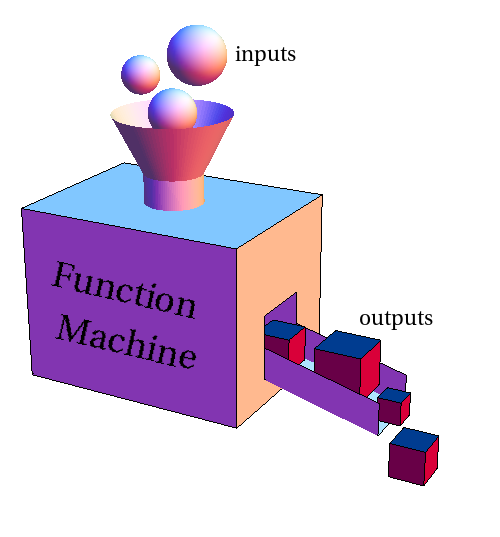
\includegraphics{images/function_machine} 

}

\caption{Ilustración de una función, tomada de www.mathinsight.org.}\label{fig:machine1}
\end{figure}

Las funciones en \proglang{R} se caracterizan por un nombre corto y que
dé una idea de lo que hace la función. Los elementos que pueden ingresar
(\emph{inputs}) a la función se llaman \textbf{parámetros} y se ubican
dentro de paréntesis, el cuerpo de la función se ubica dentro de llaves
y es ahí donde se procesan los \emph{inputs} para convertirlos en
\emph{outputs}, a continuación se muestra la estructura general de una
función.

\begin{Shaded}
\begin{Highlighting}[]
\KeywordTok{nombre_de_funcion}\NormalTok{(parametro1, parametro2, ...) \{}
  \NormalTok{tareas internas}
  \NormalTok{tareas internas}
  \NormalTok{tareas internas}
  \NormalTok{salida}
\NormalTok{\}}
\end{Highlighting}
\end{Shaded}

Cuando usamos una función sólo debemos escribir bien el nombre e
ingresar correctamente los parámetros de la función, el cuerpo de la
función ni lo vemos ni lo debemos modificar. A continuación se presenta
un ejemplo de cómo usar la función \texttt{mean} para calcular un
promedio.

\begin{Shaded}
\begin{Highlighting}[]
\NormalTok{notas <-}\StringTok{ }\KeywordTok{c}\NormalTok{(}\FloatTok{4.0}\NormalTok{, }\FloatTok{1.3}\NormalTok{, }\FloatTok{3.8}\NormalTok{, }\FloatTok{2.0}\NormalTok{)  }\CommentTok{# Notas de un estudiante}
\KeywordTok{mean}\NormalTok{(notas)}
\end{Highlighting}
\end{Shaded}

\begin{verbatim}
## [1] 2.775
\end{verbatim}

\section{\texorpdfstring{Operadores de asignación
\index{asignación}}{Operadores de asignación }}\label{operadores-de-asignacion}

En \proglang{R} se pueden hacer asignación de varias formas, a
continuación se presentan los operadores disponibles para tal fin.

\begin{itemize}
\tightlist
\item
  \texttt{\textless{}-} este es el operador de asignación a izquierda,
  es el más usado y recomendado.
\item
  \texttt{-\textgreater{}} este es el operador de asignación a derecha,
  no es frecuente su uso.
\item
  \texttt{=} el símbolo igual sirve para hacer asignaciones pero
  \textbf{NO} se recomienda usarlo.
\item
  \texttt{\textless{}\textless{}-} este es un operador de asignación
  global y sólo debe ser usado por usuarios avanzados.
\end{itemize}

\subsection*{Ejemplo}\label{ejemplo-5}


Almacene los valores 5.3, 4.6 y 25 en los objetos \texttt{a}, \texttt{b}
y \texttt{age} respectivamente, use diferentes símbolos de asignación.

Para hacer lo solicitado se podría usar el siguiente código.

\begin{Shaded}
\begin{Highlighting}[]
\NormalTok{a <-}\StringTok{ }\FloatTok{5.3} \CommentTok{# Recomended}
\FloatTok{4.6} \NormalTok{->}\StringTok{ }\NormalTok{b }\CommentTok{# It is not usual}
\NormalTok{age =}\StringTok{ }\DecValTok{25} \CommentTok{# Not recomended}
\end{Highlighting}
\end{Shaded}

\BeginKnitrBlock{rmdimportant}
Aunque una asignación se puede hacer de tres formas diferentes, se
recomienda sólo usar el símbolo \texttt{\textless{}-}.
\EndKnitrBlock{rmdimportant}

\section{\texorpdfstring{Operaciones básicas
\index{operaciones básicas}}{Operaciones básicas }}\label{operaciones-basicas}

En \proglang{R} se pueden hacer diversas operaciones usando operadores
binarios. Este tipo de operadores se denomina binarios porque actuan
entre dos objetos, a continuación el listado.

\begin{itemize}
\tightlist
\item
  \texttt{+} operador binario para sumar.
\item
  \texttt{-} operador binario para restar.
\item
  \texttt{*} operador binario para multiplicar.
\item
  \texttt{/} operador binario para dividir.
\item
  \texttt{\^{}} operador binario para potencia.
\item
  \texttt{\%/\%} operador binario para obtener el cociente en una
  división (número entero).
\item
  \texttt{\%\%} operador binario para obtener el residuo en una
  división.
\end{itemize}

A continuación se presentan ejemplos de cómo usar las anteriores
funciones.

\begin{Shaded}
\begin{Highlighting}[]
\DecValTok{6} \NormalTok{+}\StringTok{ }\DecValTok{4}  \CommentTok{# Para sumar dos números}
\end{Highlighting}
\end{Shaded}

\begin{verbatim}
## [1] 10
\end{verbatim}

\begin{Shaded}
\begin{Highlighting}[]
\NormalTok{a <-}\StringTok{ }\KeywordTok{c}\NormalTok{(}\DecValTok{1}\NormalTok{, }\DecValTok{3}\NormalTok{, }\DecValTok{2}\NormalTok{)}
\NormalTok{b <-}\StringTok{ }\KeywordTok{c}\NormalTok{(}\DecValTok{2}\NormalTok{, }\DecValTok{0}\NormalTok{, }\DecValTok{1}\NormalTok{)  }\CommentTok{# a y b de la misma dimensión}
\NormalTok{a +}\StringTok{ }\NormalTok{b  }\CommentTok{# Para sumar los vectores a y b miembro a miembro}
\end{Highlighting}
\end{Shaded}

\begin{verbatim}
## [1] 3 3 3
\end{verbatim}

\begin{Shaded}
\begin{Highlighting}[]
\NormalTok{a -}\StringTok{ }\NormalTok{b  }\CommentTok{# Para restar dos vectores a y b miembro a miembro}
\end{Highlighting}
\end{Shaded}

\begin{verbatim}
## [1] -1  3  1
\end{verbatim}

\begin{Shaded}
\begin{Highlighting}[]
\NormalTok{a *}\StringTok{ }\NormalTok{b  }\CommentTok{# Para multiplicar}
\end{Highlighting}
\end{Shaded}

\begin{verbatim}
## [1] 2 0 2
\end{verbatim}

\begin{Shaded}
\begin{Highlighting}[]
\NormalTok{a /}\StringTok{ }\NormalTok{b  }\CommentTok{# Para dividir}
\end{Highlighting}
\end{Shaded}

\begin{verbatim}
## [1] 0.5 Inf 2.0
\end{verbatim}

\begin{Shaded}
\begin{Highlighting}[]
\NormalTok{a ^}\StringTok{ }\NormalTok{b  }\CommentTok{# Para potencia}
\end{Highlighting}
\end{Shaded}

\begin{verbatim}
## [1] 1 1 2
\end{verbatim}

\begin{Shaded}
\begin{Highlighting}[]
\DecValTok{7} \NormalTok\StringTok{ }\DecValTok{3}  \CommentTok{# Para saber las veces que cabe 3 en 7}
\end{Highlighting}
\end{Shaded}

\begin{verbatim}
## [1] 2
\end{verbatim}

\begin{Shaded}
\begin{Highlighting}[]
\DecValTok{7} \NormalTok\StringTok{ }\DecValTok{3}  \CommentTok{# Para saber el residuo al dividir 7 entre 3}
\end{Highlighting}
\end{Shaded}

\begin{verbatim}
## [1] 1
\end{verbatim}

\section{\texorpdfstring{Pruebas lógicas
\index{pruebas lógicas}}{Pruebas lógicas }}\label{pruebas-logicas}

En \proglang{R} se puede verificar si un objeto cumple una condición
dada, a continuación el listado de las pruebas usuales.

\begin{itemize}
\tightlist
\item
  \texttt{\textless{}} para saber si un número es menor que otro.
\item
  \texttt{\textgreater{}} para saber si un número es mayor que otro.
\item
  \texttt{==} para saber si un número es igual que otro.
\item
  \texttt{\textless{}=} para saber si un número es menor o igual que
  otro.
\item
  \texttt{\textgreater{}=} para saber si un número es mayor o igual que
  otro.
\end{itemize}

A continuación se presentan ejemplos de cómo usar las anteriores
funciones.

\begin{Shaded}
\begin{Highlighting}[]
\DecValTok{5} \NormalTok{<}\StringTok{ }\DecValTok{12}  \CommentTok{# ¿Será 5 menor que 12?}
\end{Highlighting}
\end{Shaded}

\begin{verbatim}
## [1] TRUE
\end{verbatim}

\begin{Shaded}
\begin{Highlighting}[]
\CommentTok{# Comparando objetos}
\NormalTok{x <-}\StringTok{ }\DecValTok{5}
\NormalTok{y <-}\StringTok{ }\DecValTok{20} \NormalTok{/}\StringTok{ }\DecValTok{4}
\NormalTok{x ==}\StringTok{ }\NormalTok{y  }\CommentTok{# ¿Será x igual a y?}
\end{Highlighting}
\end{Shaded}

\begin{verbatim}
## [1] TRUE
\end{verbatim}

\begin{Shaded}
\begin{Highlighting}[]
\CommentTok{# Usando vectores}
\NormalTok{a <-}\StringTok{ }\KeywordTok{c}\NormalTok{(}\DecValTok{1}\NormalTok{, }\DecValTok{3}\NormalTok{, }\DecValTok{2}\NormalTok{)}
\NormalTok{b <-}\StringTok{ }\KeywordTok{c}\NormalTok{(}\DecValTok{2}\NormalTok{, }\DecValTok{0}\NormalTok{, }\DecValTok{1}\NormalTok{)}
\NormalTok{a >}\StringTok{ }\NormalTok{b  }\CommentTok{# Comparación término a término}
\end{Highlighting}
\end{Shaded}

\begin{verbatim}
## [1] FALSE  TRUE  TRUE
\end{verbatim}

\begin{Shaded}
\begin{Highlighting}[]
\NormalTok{a ==}\StringTok{ }\NormalTok{b  }\CommentTok{# Comparación de igualdad término a término}
\end{Highlighting}
\end{Shaded}

\begin{verbatim}
## [1] FALSE FALSE FALSE
\end{verbatim}

\subsection*{Ejemplo}\label{ejemplo-6}


Crear un vector con los números de 1 a 17 y extrater los números que son
mayores o iguales a 12.

Primero se crear el vector \texttt{x} con los elementos del 1 al 17. La
prueba lógica \texttt{x\ \textgreater{}=\ 12} se usa para evaluar la
condición, el resultado es un vector de 17 posiciones con valores de
\texttt{TRUE} o \texttt{FALSE} dependiendo de si la condición se cumple
o no. Este vector lógico se coloca dentro de \texttt{x{[}\ {]}} para que
al evaluar \texttt{x{[}x\ \textgreater{}=\ 12{]}} sólo aparezcan los
valores del vector original que SI cumplen la condición. El código
necesario se muestra a continuación.

\begin{Shaded}
\begin{Highlighting}[]
\NormalTok{x <-}\StringTok{ }\DecValTok{1}\NormalTok{:}\DecValTok{17}  \CommentTok{# Se crea el vector}
\NormalTok{x[x >=}\StringTok{ }\DecValTok{12}\NormalTok{]  }\CommentTok{# Se solicitan los valores que cumplen la condición}
\end{Highlighting}
\end{Shaded}

\begin{verbatim}
## [1] 12 13 14 15 16 17
\end{verbatim}

\subsection*{Ejemplo}\label{ejemplo-7}


Retome el marco de datos \texttt{mimarco} construído en la sección
\ref{marcodatos} y use una prueba lógica para extraer la información de
las personas que tienen una edad superior o igual a 15 años.

Inicialmente vamos a construir nuevamente el objeto \texttt{mimarco} de
la sección \ref{marcodatos} usando el siguiente código.

\begin{Shaded}
\begin{Highlighting}[]
\NormalTok{mimarco <-}\StringTok{ }\KeywordTok{data.frame}\NormalTok{(}\DataTypeTok{edad =} \KeywordTok{c}\NormalTok{(}\DecValTok{15}\NormalTok{, }\DecValTok{19}\NormalTok{, }\DecValTok{13}\NormalTok{, }\OtherTok{NA}\NormalTok{, }\DecValTok{20}\NormalTok{), }
                      \DataTypeTok{deporte =} \KeywordTok{c}\NormalTok{(}\OtherTok{TRUE}\NormalTok{, }\OtherTok{TRUE}\NormalTok{, }\OtherTok{NA}\NormalTok{, }\OtherTok{FALSE}\NormalTok{, }\OtherTok{TRUE}\NormalTok{),}
                      \DataTypeTok{comic.fav =} \KeywordTok{c}\NormalTok{(}\OtherTok{NA}\NormalTok{, }\StringTok{'Superman'}\NormalTok{, }\StringTok{'Batman'}\NormalTok{,}
                                    \OtherTok{NA}\NormalTok{, }\StringTok{'Batman'}\NormalTok{))}

\NormalTok{mimarco  }\CommentTok{# Para ver el contenido de mimarco}
\end{Highlighting}
\end{Shaded}

\begin{verbatim}
##   edad deporte comic.fav
## 1   15    TRUE      <NA>
## 2   19    TRUE  Superman
## 3   13      NA    Batman
## 4   NA   FALSE      <NA>
## 5   20    TRUE    Batman
\end{verbatim}

Para extraer de \texttt{mimarco} la información de las personas que
tienen una edad superior o igual a 15 años se coloca dentro de corchetes
la condición \texttt{mimarco\$edad\ \textgreater{}=\ 15}, esto servirá
para chequear cuáles de las edades del vector \texttt{mimarco\$ead}
cumplen la condición. El resultado de evaluar
\texttt{mimarco\$edad\ \textgreater{}=\ 15} será un vector lógico
(\texttt{TRUE} o \texttt{FALSE}), que al ser colocado dentro de
\texttt{mimarco{[},{]}}, entregará la información de las personas que
cumplen la condición. A continuación el código para extraer la
información solicitada.

\begin{Shaded}
\begin{Highlighting}[]
\NormalTok{mimarco[mimarco$edad >=}\StringTok{ }\DecValTok{15}\NormalTok{, ]}
\end{Highlighting}
\end{Shaded}

\begin{verbatim}
##    edad deporte comic.fav
## 1    15    TRUE      <NA>
## 2    19    TRUE  Superman
## NA   NA      NA      <NA>
## 5    20    TRUE    Batman
\end{verbatim}

De la salida anterior se observa que 4 personas de las 5 cumplean la
condición.

\BeginKnitrBlock{rmdwarning}
Note que la condición \texttt{mimarco\$edad\ \textgreater{}=\ 15} se
debe ubicar \textbf{antes} de la coma para obtener todos individuos que
cumplen con la condición.
\EndKnitrBlock{rmdwarning}

\section{\texorpdfstring{Operadores lógicos
\index{operadores lógicos}}{Operadores lógicos }}\label{operadores-logicos}

En \proglang{R} están disponibles los operadores lógicos negación,
conjunción y disyunción. A continuación el listado de los operadores
entre los elementos \texttt{x} e \texttt{y}.

\begin{Shaded}
\begin{Highlighting}[]
\NormalTok{!x  }\CommentTok{# Negación de x}
\NormalTok{x &}\StringTok{ }\NormalTok{y  }\CommentTok{# Conjunción entre x e y}
\NormalTok{x &&}\StringTok{ }\NormalTok{y}
\NormalTok{x |}\StringTok{ }\NormalTok{y  }\CommentTok{# Disyunción entre x e y}
\NormalTok{x ||}\StringTok{ }\NormalTok{y}
\KeywordTok{xor}\NormalTok{(x, y)}
\end{Highlighting}
\end{Shaded}

A continuación se presentan ejemplos de cómo usar el símbolo de negación
\texttt{!}.

\begin{Shaded}
\begin{Highlighting}[]
\NormalTok{ans <-}\StringTok{ }\KeywordTok{c}\NormalTok{(}\OtherTok{TRUE}\NormalTok{, }\OtherTok{FALSE}\NormalTok{, }\OtherTok{TRUE}\NormalTok{)}
\NormalTok{!ans  }\CommentTok{# Negando las respuestas almacenadas en ans}
\end{Highlighting}
\end{Shaded}

\begin{verbatim}
## [1] FALSE  TRUE FALSE
\end{verbatim}

\begin{Shaded}
\begin{Highlighting}[]
\NormalTok{x <-}\StringTok{ }\KeywordTok{c}\NormalTok{(}\DecValTok{5}\NormalTok{, }\FloatTok{1.5}\NormalTok{, }\DecValTok{2}\NormalTok{, }\DecValTok{3}\NormalTok{, }\DecValTok{2}\NormalTok{)}
\NormalTok{!(x <}\StringTok{ }\FloatTok{2.5}\NormalTok{)  }\CommentTok{# Negando los resultados de una prueba}
\end{Highlighting}
\end{Shaded}

\begin{verbatim}
## [1]  TRUE FALSE FALSE  TRUE FALSE
\end{verbatim}

A continuación se presentan ejemplos de cómo aplicar la conjunción
\texttt{\&} y \texttt{\&\&}.

\begin{Shaded}
\begin{Highlighting}[]
\NormalTok{x <-}\StringTok{ }\KeywordTok{c}\NormalTok{(}\DecValTok{5}\NormalTok{, }\FloatTok{1.5}\NormalTok{, }\DecValTok{2}\NormalTok{)  }\CommentTok{# Se construyen dos vectores para la prueba}
\NormalTok{y <-}\StringTok{ }\KeywordTok{c}\NormalTok{(}\DecValTok{4}\NormalTok{, }\DecValTok{6}\NormalTok{, }\DecValTok{3}\NormalTok{)}

\NormalTok{x <}\StringTok{ }\DecValTok{4}  \CommentTok{# ¿Serán los elementos de x menores que 4?}
\end{Highlighting}
\end{Shaded}

\begin{verbatim}
## [1] FALSE  TRUE  TRUE
\end{verbatim}

\begin{Shaded}
\begin{Highlighting}[]
\NormalTok{y >}\StringTok{ }\DecValTok{5}  \CommentTok{# ¿Serán los elementos de y mayores que 5?}
\end{Highlighting}
\end{Shaded}

\begin{verbatim}
## [1] FALSE  TRUE FALSE
\end{verbatim}

\begin{Shaded}
\begin{Highlighting}[]
\NormalTok{x <}\StringTok{ }\DecValTok{4} \NormalTok{&}\StringTok{ }\NormalTok{y >}\StringTok{ }\DecValTok{5}  \CommentTok{# Conjunción entre las pruebas anteriores.}
\end{Highlighting}
\end{Shaded}

\begin{verbatim}
## [1] FALSE  TRUE FALSE
\end{verbatim}

\begin{Shaded}
\begin{Highlighting}[]
\NormalTok{x <}\StringTok{ }\DecValTok{4} \NormalTok{&&}\StringTok{ }\NormalTok{y >}\StringTok{ }\DecValTok{5}  \CommentTok{# Conjunción vectorial}
\end{Highlighting}
\end{Shaded}

\begin{verbatim}
## [1] FALSE
\end{verbatim}

Note las diferencias entre los dos últimos ejemplos, cuando se usa
\texttt{\&} se hace una prueba término a término y el resultado es un
vector, cuando se usa \texttt{\&\&} se aplica la conjunción al vector de
resultados obtenido con \texttt{\&}.

\subsection*{Ejemplo}\label{ejemplo-8}


Retome el marco de datos \texttt{mimarco} construído en la sección
\ref{marcodatos} y use una prueba lógica para extraer la información de
las personas que tienen una edad superior o igual a 15 años y que
practican deporte.

Aquí interesa extraer la información de los individuos que cumplen dos
condiciones simultáneamente, aquellos con edad \(\geq\) 15 y que SI
practiquen deporte. El código necesario para obtener la información
solicitada es el siguiente.

\begin{Shaded}
\begin{Highlighting}[]
\NormalTok{mimarco[mimarco$edad >=}\StringTok{ }\DecValTok{15} \NormalTok{&}\StringTok{ }\NormalTok{mimarco$deporte ==}\StringTok{ }\OtherTok{TRUE}\NormalTok{, ]}
\end{Highlighting}
\end{Shaded}

\begin{verbatim}
##   edad deporte comic.fav
## 1   15    TRUE      <NA>
## 2   19    TRUE  Superman
## 5   20    TRUE    Batman
\end{verbatim}

De la anterior salida se observa que sólo 3 de las 5 personas cumplen
ambas condiciones.

\index{with} \BeginKnitrBlock{rmdtip}

La función \texttt{with} es útil porque nos permite realizar algún
procedimiento \textbf{CON} un objeto, escribiendo menos y de una forma
más natural.
\EndKnitrBlock{rmdtip}

Una forma alternativa para escribir lo anterior usando la función
\texttt{with} es la siguiente.

\begin{Shaded}
\begin{Highlighting}[]
\KeywordTok{with}\NormalTok{(mimarco, mimarco[edad >=}\StringTok{ }\DecValTok{15} \NormalTok{&}\StringTok{ }\NormalTok{deporte ==}\StringTok{ }\OtherTok{TRUE}\NormalTok{, ])}
\end{Highlighting}
\end{Shaded}

\begin{verbatim}
##   edad deporte comic.fav
## 1   15    TRUE      <NA>
## 2   19    TRUE  Superman
## 5   20    TRUE    Batman
\end{verbatim}

Al usar \texttt{with} sólo se tuvo que escribir el objeto
\texttt{mimarco} dos veces. Cuando hay muchas condiciones o cuando el
objeto tiene un nombre largo es aconsejable usar \texttt{with}.

\section{Funciones sobre vectores}\label{funciones-sobre-vectores}

En \proglang{R} podemos destacar las siguientes funciones básicas sobre
vectores numéricos.

\index{min} \index{max} \index{legth} \index{range} \index{sum}
\index{prod} \index{which.min} \index{which.max}

\begin{itemize}
\tightlist
\item
  \texttt{min}: para obtener el mínimo de un vector.
\item
  \texttt{max}: para obtener el máximo de un vector.
\item
  \texttt{length}: para determinar la longitud de un vector.
\item
  \texttt{range}: para obtener el rango de valores de un vector, entrega
  el mínimo y máximo.
\item
  \texttt{sum}: entrega la suma de todos los elementos del vector.
\item
  \texttt{prod}: multiplica todos los elementos del vector.
\item
  \texttt{which.min}: nos entrega la posición en donde está el valor
  mínimo del vector.
\item
  \texttt{which.max}: nos da la posición del valor máximo del vector.
\item
  \texttt{rev}: invierte un vector.
\end{itemize}

\subsection*{Ejemplo}\label{ejemplo-9}


Construir en vector llamado \texttt{myvec} con los siguientes elementos:
5, 3, 2, 1, 2, 0, NA, 0, 9, 6. Luego aplicar todas las funciones
anteriores para verificar el funcionamiento de las mismas.

\begin{Shaded}
\begin{Highlighting}[]
\NormalTok{myvec <-}\StringTok{ }\KeywordTok{c}\NormalTok{(}\DecValTok{5}\NormalTok{, }\DecValTok{3}\NormalTok{, }\DecValTok{2}\NormalTok{, }\DecValTok{1}\NormalTok{, }\DecValTok{2}\NormalTok{, }\DecValTok{0}\NormalTok{, }\OtherTok{NA}\NormalTok{, }\DecValTok{0}\NormalTok{, }\DecValTok{9}\NormalTok{, }\DecValTok{6}\NormalTok{)}
\NormalTok{myvec}
\end{Highlighting}
\end{Shaded}

\begin{verbatim}
##  [1]  5  3  2  1  2  0 NA  0  9  6
\end{verbatim}

\begin{Shaded}
\begin{Highlighting}[]
\KeywordTok{min}\NormalTok{(myvec)  }\CommentTok{# Opss, no aparece el mínimo que es Cero.}
\end{Highlighting}
\end{Shaded}

\begin{verbatim}
## [1] NA
\end{verbatim}

\begin{Shaded}
\begin{Highlighting}[]
\KeywordTok{min}\NormalTok{(myvec, }\DataTypeTok{na.rm=}\OtherTok{TRUE}\NormalTok{)  }\CommentTok{# Usamos na.rm = TRUE para remover el NA}
\end{Highlighting}
\end{Shaded}

\begin{verbatim}
## [1] 0
\end{verbatim}

\begin{Shaded}
\begin{Highlighting}[]
\KeywordTok{max}\NormalTok{(myvec, }\DataTypeTok{na.rm=}\NormalTok{T)  }\CommentTok{# Para obtener el valor máximo}
\end{Highlighting}
\end{Shaded}

\begin{verbatim}
## [1] 9
\end{verbatim}

\begin{Shaded}
\begin{Highlighting}[]
\KeywordTok{range}\NormalTok{(myvec, }\DataTypeTok{na.rm=}\NormalTok{T)  }\CommentTok{# Genera min y max simultáneamente}
\end{Highlighting}
\end{Shaded}

\begin{verbatim}
## [1] 0 9
\end{verbatim}

\begin{Shaded}
\begin{Highlighting}[]
\KeywordTok{sum}\NormalTok{(myvec, }\DataTypeTok{na.rm=}\NormalTok{T)  }\CommentTok{# La suma de los valores internos}
\end{Highlighting}
\end{Shaded}

\begin{verbatim}
## [1] 28
\end{verbatim}

\begin{Shaded}
\begin{Highlighting}[]
\KeywordTok{prod}\NormalTok{(myvec, }\DataTypeTok{na.rm=}\NormalTok{T)  }\CommentTok{# El productor de los valores internos}
\end{Highlighting}
\end{Shaded}

\begin{verbatim}
## [1] 0
\end{verbatim}

\begin{Shaded}
\begin{Highlighting}[]
\KeywordTok{which.min}\NormalTok{(myvec)  }\CommentTok{# Posición del valor mínimo 0 en el vector}
\end{Highlighting}
\end{Shaded}

\begin{verbatim}
## [1] 6
\end{verbatim}

\begin{Shaded}
\begin{Highlighting}[]
\KeywordTok{which.max}\NormalTok{(myvec)  }\CommentTok{# Posición del valor máximo 9 en el vector}
\end{Highlighting}
\end{Shaded}

\begin{verbatim}
## [1] 9
\end{verbatim}

De las dos últimas líneas podemos destacar lo siguiente:

\begin{enumerate}
\def\labelenumi{\arabic{enumi}.}
\tightlist
\item
  \textbf{NO es necesario} usar \texttt{na.rm\ =\ TRUE} para remover el
  \texttt{NA} dentro de las funciones \texttt{which.min} ni
  \texttt{which.max}.
\item
  El valor mínimo 0 aparece en las posiciones 6 y 8 pero la función
  \texttt{which.min} sólo entrega la posición del primer valor mínimo
  dentro del vector.
\end{enumerate}

\section{Funciones matemáticas}\label{funciones-matematicas}

Otras funciones básicas muy utilizadas en estadística son:
\texttt{sin,\ cos,\ tan,\ asin,\ acos,\ atan,\ atan2,\ log,\ logb,\ log10,\ exp,\ sqrt,\ abs}.
A continuación algunos ejemplos de las anteriores funciones.

\textbf{Ejemplos de medidas trigonométricas}

\begin{Shaded}
\begin{Highlighting}[]
\NormalTok{angulos <-}\StringTok{ }\KeywordTok{c}\NormalTok{(}\DecValTok{0}\NormalTok{, pi/}\DecValTok{2}\NormalTok{, pi)}
\KeywordTok{sin}\NormalTok{(angulos)}
\end{Highlighting}
\end{Shaded}

\begin{verbatim}
## [1] 0.000e+00 1.000e+00 1.225e-16
\end{verbatim}

\begin{Shaded}
\begin{Highlighting}[]
\KeywordTok{tan}\NormalTok{(angulos)}
\end{Highlighting}
\end{Shaded}

\begin{verbatim}
## [1]  0.000e+00  1.633e+16 -1.225e-16
\end{verbatim}

\textbf{Ejemplos de logaritmos}

\begin{Shaded}
\begin{Highlighting}[]
\KeywordTok{log}\NormalTok{(}\DecValTok{100}\NormalTok{)}
\end{Highlighting}
\end{Shaded}

\begin{verbatim}
## [1] 4.605
\end{verbatim}

\begin{Shaded}
\begin{Highlighting}[]
\KeywordTok{log10}\NormalTok{(}\DecValTok{100}\NormalTok{)}
\end{Highlighting}
\end{Shaded}

\begin{verbatim}
## [1] 2
\end{verbatim}

\begin{Shaded}
\begin{Highlighting}[]
\KeywordTok{logb}\NormalTok{(}\DecValTok{125}\NormalTok{, }\DataTypeTok{base=}\DecValTok{5}\NormalTok{)}
\end{Highlighting}
\end{Shaded}

\begin{verbatim}
## [1] 3
\end{verbatim}

\textbf{Ejemplos de exponencial}

\begin{Shaded}
\begin{Highlighting}[]
\KeywordTok{exp}\NormalTok{(}\DecValTok{1}\NormalTok{)}
\end{Highlighting}
\end{Shaded}

\begin{verbatim}
## [1] 2.718
\end{verbatim}

\begin{Shaded}
\begin{Highlighting}[]
\KeywordTok{exp}\NormalTok{(}\DecValTok{2}\NormalTok{)}
\end{Highlighting}
\end{Shaded}

\begin{verbatim}
## [1] 7.389
\end{verbatim}

\begin{Shaded}
\begin{Highlighting}[]
\KeywordTok{exp}\NormalTok{(}\DecValTok{1}\NormalTok{:}\DecValTok{3}\NormalTok{)}
\end{Highlighting}
\end{Shaded}

\begin{verbatim}
## [1]  2.718  7.389 20.086
\end{verbatim}

\textbf{Ejemplos de raices}

\begin{Shaded}
\begin{Highlighting}[]
\KeywordTok{sqrt}\NormalTok{(}\DecValTok{49}\NormalTok{)  }\CommentTok{# Raiz cuadrada de 49}
\end{Highlighting}
\end{Shaded}

\begin{verbatim}
## [1] 7
\end{verbatim}

\begin{Shaded}
\begin{Highlighting}[]
\DecValTok{27} \NormalTok{^}\StringTok{ }\NormalTok{(}\DecValTok{1}\NormalTok{/}\DecValTok{3}\NormalTok{)  }\CommentTok{# Raiz cúbica de 27}
\end{Highlighting}
\end{Shaded}

\begin{verbatim}
## [1] 3
\end{verbatim}

\textbf{Ejemplos de valor absoluto}

\begin{Shaded}
\begin{Highlighting}[]
\KeywordTok{abs}\NormalTok{(}\FloatTok{2.5}\NormalTok{)}
\end{Highlighting}
\end{Shaded}

\begin{verbatim}
## [1] 2.5
\end{verbatim}

\begin{Shaded}
\begin{Highlighting}[]
\KeywordTok{abs}\NormalTok{(-}\FloatTok{3.6}\NormalTok{)}
\end{Highlighting}
\end{Shaded}

\begin{verbatim}
## [1] 3.6
\end{verbatim}

\section{\texorpdfstring{Función \texttt{seq} \index{seq}
\index{secuencias}}{Función seq  }}\label{funcion-seq}

En \proglang{R} podemos crear secuencias de números de una forma
sencilla usando la función \texttt{seq}, la estructura de esta función
es:

\begin{Shaded}
\begin{Highlighting}[]
\KeywordTok{seq}\NormalTok{(}\DataTypeTok{from=}\DecValTok{1}\NormalTok{, }\DataTypeTok{to=}\DecValTok{1}\NormalTok{, by, length.out)}
\end{Highlighting}
\end{Shaded}

Los argumentos de esta función son:

\begin{itemize}
\tightlist
\item
  \texttt{from}: valor de inicio de la secuencia.
\item
  \texttt{to}: valor de fin de la secuencia, no siempre se alcanza.
\item
  \texttt{by}: incremento de la secuencia.
\item
  \texttt{length.out}: longitud deseado de la secuencia.
\end{itemize}

\subsection*{Ejemplo}\label{ejemplo-10}


Construya las siguientes tres secuencias usando la función \texttt{seq}.

\begin{itemize}
\tightlist
\item
  Once valores igualmente espaciados desde 0 hasta 1.
\item
  Una secuencia de dos en dos comenzando en 1.
\item
  Una secuencia desde 1 con un salto de \(\pi\) y sin pasar del número
  9.
\end{itemize}

El código necesario para obtener las secuencias se muestra a
continuación.

\begin{Shaded}
\begin{Highlighting}[]
\KeywordTok{seq}\NormalTok{(}\DataTypeTok{from=}\DecValTok{0}\NormalTok{, }\DataTypeTok{to=}\DecValTok{1}\NormalTok{, }\DataTypeTok{length.out =} \DecValTok{11}\NormalTok{)}
\end{Highlighting}
\end{Shaded}

\begin{verbatim}
##  [1] 0.0 0.1 0.2 0.3 0.4 0.5 0.6 0.7 0.8 0.9 1.0
\end{verbatim}

\begin{Shaded}
\begin{Highlighting}[]
\KeywordTok{seq}\NormalTok{(}\DataTypeTok{from=}\DecValTok{1}\NormalTok{, }\DataTypeTok{to=}\DecValTok{9}\NormalTok{, }\DataTypeTok{by=}\DecValTok{2}\NormalTok{)  }\CommentTok{# matches 'end'}
\end{Highlighting}
\end{Shaded}

\begin{verbatim}
## [1] 1 3 5 7 9
\end{verbatim}

\begin{Shaded}
\begin{Highlighting}[]
\KeywordTok{seq}\NormalTok{(}\DataTypeTok{from=}\DecValTok{1}\NormalTok{, }\DataTypeTok{to=}\DecValTok{9}\NormalTok{, }\DataTypeTok{by=}\NormalTok{pi) }\CommentTok{# stays below 'end'}
\end{Highlighting}
\end{Shaded}

\begin{verbatim}
## [1] 1.000 4.142 7.283
\end{verbatim}

\BeginKnitrBlock{rmdnote}
En \proglang{R} existe el operador binario \texttt{:} que sirve para
construir secuencias de uno en uno fácilmente.
\EndKnitrBlock{rmdnote}

Revise los siguientes ejemplos para entender el funcionamiento del
operador \texttt{:}.

\begin{Shaded}
\begin{Highlighting}[]
\DecValTok{2}\NormalTok{:}\DecValTok{8}
\end{Highlighting}
\end{Shaded}

\begin{verbatim}
## [1] 2 3 4 5 6 7 8
\end{verbatim}

\begin{Shaded}
\begin{Highlighting}[]
\DecValTok{3}\NormalTok{:-}\DecValTok{5}
\end{Highlighting}
\end{Shaded}

\begin{verbatim}
## [1]  3  2  1  0 -1 -2 -3 -4 -5
\end{verbatim}

\begin{Shaded}
\begin{Highlighting}[]
\NormalTok{pi:}\DecValTok{6}  \CommentTok{# real sequence}
\end{Highlighting}
\end{Shaded}

\begin{verbatim}
## [1] 3.142 4.142 5.142
\end{verbatim}

\begin{Shaded}
\begin{Highlighting}[]
\DecValTok{6}\NormalTok{:pi  }\CommentTok{# integer sequence}
\end{Highlighting}
\end{Shaded}

\begin{verbatim}
## [1] 6 5 4
\end{verbatim}

\section{\texorpdfstring{Función \texttt{rep} \index{rep}
\index{repeticiones}}{Función rep  }}\label{funcion-rep}

En \proglang{R} podemos crear repeticiones usando la función
\texttt{rep}, la estructura de esta función es:

\begin{Shaded}
\begin{Highlighting}[]
\KeywordTok{rep}\NormalTok{(x, }\DataTypeTok{times=}\DecValTok{1}\NormalTok{, }\DataTypeTok{length.out=}\OtherTok{NA}\NormalTok{, }\DataTypeTok{each=}\DecValTok{1}\NormalTok{)}
\end{Highlighting}
\end{Shaded}

Los argumentos de esta función son:

\begin{itemize}
\tightlist
\item
  \texttt{x}: vector con los elementos a repetir.
\item
  \texttt{times}: número de veces que el vector \texttt{x} se debe
  repetir.
\item
  \texttt{length.out}: longitud deseada para el vector resultante.
\item
  \texttt{each}: número de veces que cada elemento de \texttt{x} se debe
  repetir.
\end{itemize}

\subsection*{Ejemplo}\label{ejemplo-11}


Construya las siguientes repeticiones usando la función \texttt{rep}, no
lo haga ingresando número por número.

\begin{itemize}
\tightlist
\item
  1 2 3 4 1 2 3 4
\item
  1 1 2 2 3 3 4 4
\item
  1 1 2 3 3 4
\item
  1 1 2 2 3 3 4 4
\end{itemize}

La clave para construir una repetición es descrubir la semilla o
elemento que se repite. Las instrucciones para obtener las repeticiones
anteriores se muestra a continuación.

\begin{Shaded}
\begin{Highlighting}[]
\KeywordTok{rep}\NormalTok{(}\DataTypeTok{x=}\DecValTok{1}\NormalTok{:}\DecValTok{4}\NormalTok{, }\DataTypeTok{times=}\DecValTok{2}\NormalTok{)}
\end{Highlighting}
\end{Shaded}

\begin{verbatim}
## [1] 1 2 3 4 1 2 3 4
\end{verbatim}

\begin{Shaded}
\begin{Highlighting}[]
\KeywordTok{rep}\NormalTok{(}\DataTypeTok{x=}\DecValTok{1}\NormalTok{:}\DecValTok{4}\NormalTok{, }\DataTypeTok{times=}\KeywordTok{c}\NormalTok{(}\DecValTok{2}\NormalTok{,}\DecValTok{2}\NormalTok{,}\DecValTok{2}\NormalTok{,}\DecValTok{2}\NormalTok{))}
\end{Highlighting}
\end{Shaded}

\begin{verbatim}
## [1] 1 1 2 2 3 3 4 4
\end{verbatim}

\begin{Shaded}
\begin{Highlighting}[]
\KeywordTok{rep}\NormalTok{(}\DataTypeTok{x=}\DecValTok{1}\NormalTok{:}\DecValTok{4}\NormalTok{, }\DataTypeTok{times=}\KeywordTok{c}\NormalTok{(}\DecValTok{2}\NormalTok{,}\DecValTok{1}\NormalTok{,}\DecValTok{2}\NormalTok{,}\DecValTok{1}\NormalTok{))}
\end{Highlighting}
\end{Shaded}

\begin{verbatim}
## [1] 1 1 2 3 3 4
\end{verbatim}

\begin{Shaded}
\begin{Highlighting}[]
\KeywordTok{rep}\NormalTok{(}\DataTypeTok{x=}\DecValTok{1}\NormalTok{:}\DecValTok{4}\NormalTok{, }\DataTypeTok{each=}\DecValTok{2}\NormalTok{)}
\end{Highlighting}
\end{Shaded}

\begin{verbatim}
## [1] 1 1 2 2 3 3 4 4
\end{verbatim}

\subsection*{Ejemplo}\label{ejemplo-12}


La función \texttt{rep} es muy versátil, observe los siguientes 4
ejemplos y saque una conclusión de cada uno de ellos.

\begin{Shaded}
\begin{Highlighting}[]
\KeywordTok{rep}\NormalTok{(}\DataTypeTok{x=}\DecValTok{1}\NormalTok{:}\DecValTok{4}\NormalTok{, }\DataTypeTok{each=}\DecValTok{2}\NormalTok{)}
\end{Highlighting}
\end{Shaded}

\begin{verbatim}
## [1] 1 1 2 2 3 3 4 4
\end{verbatim}

\begin{Shaded}
\begin{Highlighting}[]
\KeywordTok{rep}\NormalTok{(}\DataTypeTok{x=}\DecValTok{1}\NormalTok{:}\DecValTok{4}\NormalTok{, }\DataTypeTok{each=}\DecValTok{2}\NormalTok{, }\DataTypeTok{len=}\DecValTok{4}\NormalTok{)    }\CommentTok{# first 4 only.}
\end{Highlighting}
\end{Shaded}

\begin{verbatim}
## [1] 1 1 2 2
\end{verbatim}

\begin{Shaded}
\begin{Highlighting}[]
\KeywordTok{rep}\NormalTok{(}\DataTypeTok{x=}\DecValTok{1}\NormalTok{:}\DecValTok{4}\NormalTok{, }\DataTypeTok{each=}\DecValTok{2}\NormalTok{, }\DataTypeTok{len=}\DecValTok{10}\NormalTok{)   }\CommentTok{# 8 integers plus two recycled 1's.}
\end{Highlighting}
\end{Shaded}

\begin{verbatim}
##  [1] 1 1 2 2 3 3 4 4 1 1
\end{verbatim}

\begin{Shaded}
\begin{Highlighting}[]
\KeywordTok{rep}\NormalTok{(}\DataTypeTok{x=}\DecValTok{1}\NormalTok{:}\DecValTok{4}\NormalTok{, }\DataTypeTok{each=}\DecValTok{2}\NormalTok{, }\DataTypeTok{times=}\DecValTok{3}\NormalTok{)  }\CommentTok{# length 24, 3 complete replications}
\end{Highlighting}
\end{Shaded}

\begin{verbatim}
##  [1] 1 1 2 2 3 3 4 4 1 1 2 2 3 3 4 4 1 1 2 2 3 3 4 4
\end{verbatim}

\section{\texorpdfstring{Funciones \texttt{round}, \texttt{ceiling},
\texttt{floor} y \texttt{trunc} \index{round} \index{ceiling}
\index{floor}
\index{trunc}}{Funciones round, ceiling, floor y trunc    }}\label{funciones-round-ceiling-floor-y-trunc}

Existen 4 funciones útiles para modificar u obtener información de un
número, estas funciones son \texttt{round}, \texttt{ceiling},
\texttt{floor} y \texttt{trunc}.

\begin{itemize}
\tightlist
\item
  \texttt{round(x,\ digits)}: sirve para redondear un número según los
  dígitos indicados.
\item
  \texttt{ceiling(x)}: entrega el mínimo entero mayor o igual que
  \texttt{x}.
\item
  \texttt{floor(x)}: entrega el máximo entero menor o igual que
  \texttt{x}.
\item
  \texttt{trunc(x)}: entrega la parte entera de un número \texttt{x}.
\end{itemize}

\subsection*{Ejemplo}\label{ejemplo-13}


Aplique las funciones \texttt{round}, \texttt{ceiling}, \texttt{floor} y
\texttt{trunc} a un valor positivo y a un valor negativo para
inspeccionar los resultados.

A continuación el código de prueba para un número positivo cualquiera.

\begin{Shaded}
\begin{Highlighting}[]
\NormalTok{x <-}\StringTok{ }\FloatTok{5.34896}  \CommentTok{# Número positivo elegido}
\KeywordTok{round}\NormalTok{(x, }\DataTypeTok{digits=}\DecValTok{3}\NormalTok{)}
\end{Highlighting}
\end{Shaded}

\begin{verbatim}
## [1] 5.349
\end{verbatim}

\begin{Shaded}
\begin{Highlighting}[]
\KeywordTok{ceiling}\NormalTok{(x)}
\end{Highlighting}
\end{Shaded}

\begin{verbatim}
## [1] 6
\end{verbatim}

\begin{Shaded}
\begin{Highlighting}[]
\KeywordTok{floor}\NormalTok{(x)}
\end{Highlighting}
\end{Shaded}

\begin{verbatim}
## [1] 5
\end{verbatim}

\begin{Shaded}
\begin{Highlighting}[]
\KeywordTok{trunc}\NormalTok{(x)}
\end{Highlighting}
\end{Shaded}

\begin{verbatim}
## [1] 5
\end{verbatim}

A continuación las pruebas con un número negativo cualquiera.

\begin{Shaded}
\begin{Highlighting}[]
\NormalTok{x <-}\StringTok{ }\NormalTok{-}\FloatTok{4.26589}  \CommentTok{# Número negativo elegido}
\KeywordTok{round}\NormalTok{(x, }\DataTypeTok{digits=}\DecValTok{3}\NormalTok{)}
\end{Highlighting}
\end{Shaded}

\begin{verbatim}
## [1] -4.266
\end{verbatim}

\begin{Shaded}
\begin{Highlighting}[]
\KeywordTok{ceiling}\NormalTok{(x)}
\end{Highlighting}
\end{Shaded}

\begin{verbatim}
## [1] -4
\end{verbatim}

\begin{Shaded}
\begin{Highlighting}[]
\KeywordTok{floor}\NormalTok{(x)}
\end{Highlighting}
\end{Shaded}

\begin{verbatim}
## [1] -5
\end{verbatim}

\begin{Shaded}
\begin{Highlighting}[]
\KeywordTok{trunc}\NormalTok{(x)}
\end{Highlighting}
\end{Shaded}

\begin{verbatim}
## [1] -4
\end{verbatim}

\section{\texorpdfstring{Funciones \texttt{sort} y \texttt{rank}
\index{sort} \index{rank} \index{ordenar}
\index{posición}}{Funciones sort y rank    }}\label{funciones-sort-y-rank}

Las funciones \texttt{sort} y \texttt{rank} son útiles para ordenar los
elementos de un vector o para saber las posiciones que ocuarían los
elementos de un vector al ser ordenado. La estructura de las dos
funciones es la siguiente.

\begin{Shaded}
\begin{Highlighting}[]
\KeywordTok{sort}\NormalTok{(x, }\DataTypeTok{decreasing =} \OtherTok{FALSE}\NormalTok{)}
\KeywordTok{rank}\NormalTok{(x)}
\end{Highlighting}
\end{Shaded}

En el parámetro \texttt{x} se ingresa el vector y el parámetro
\texttt{decreasing} sirva para indicar si el ordenamiento es de menor a
mayor (por defecto es este) o de mayor a menor.

\subsection*{Ejemplo}\label{ejemplo-14}


Considere el vector \texttt{x} que tiene los siguientes elementos: 2, 3,
6, 4, 9 y 5. Ordene el vector de menor a mayor, de mayor a menor y por
último encuentre la posición que ocupan los elementos de \texttt{x} si
se ordenaran de menor a mayor.

\begin{Shaded}
\begin{Highlighting}[]
\NormalTok{x <-}\StringTok{ }\KeywordTok{c}\NormalTok{(}\DecValTok{2}\NormalTok{, }\DecValTok{3}\NormalTok{, }\DecValTok{6}\NormalTok{, }\DecValTok{4}\NormalTok{, }\DecValTok{9}\NormalTok{, }\DecValTok{5}\NormalTok{)}
\KeywordTok{sort}\NormalTok{(x)}
\end{Highlighting}
\end{Shaded}

\begin{verbatim}
## [1] 2 3 4 5 6 9
\end{verbatim}

\begin{Shaded}
\begin{Highlighting}[]
\KeywordTok{sort}\NormalTok{(x, }\DataTypeTok{decreasing=}\OtherTok{TRUE}\NormalTok{)}
\end{Highlighting}
\end{Shaded}

\begin{verbatim}
## [1] 9 6 5 4 3 2
\end{verbatim}

\begin{Shaded}
\begin{Highlighting}[]
\KeywordTok{rank}\NormalTok{(x)}
\end{Highlighting}
\end{Shaded}

\begin{verbatim}
## [1] 1 2 5 3 6 4
\end{verbatim}

\section*{EJERCICIOS}\label{ejercicios-1}


Use funciones o procedimientos (varias líneas) de \proglang{R} para
responder cada una de las siguientes preguntas.

\begin{enumerate}
\def\labelenumi{\arabic{enumi}.}
\tightlist
\item
  ¿Qué cantidad de dinero sobra al repartir 10000\$ entre 3 personas?
\item
  ¿Es el número 4560 divisible por 3?
\item
  Construya un vector con los números enteros del 2 al 87. ¿Cuáles de
  esos números son divisibles por 7?
\item
  Construya dos vectores, el primero con los números enteros desde 7
  hasta 3, el segundo vector con los primeros cinco números positivos
  divisibles por 5. Sea A la condición de ser par en el primer vector.
  Sea B la condición de ser mayor que 10 en el segundo vector. ¿En cuál
  de las 5 posiciones se cumple A y B simultáneamente?
\item
  Consulte el siguiente enlace sobre una anéctoda de Gauss cuando tenía
  10 años de edad \url{http://tinyurl.com/hk2l8h2}. Use R para obtener
  el resultado de la suma solicitada por el profesor del niño Gauss.
\item
  Construya un vector con los siguientes elementos: 1, -4, 5, 9, -4.
  Escriba un procedimiento para extraer \textbf{las posiciones} donde
  está el valor mínimo en el vector.
\item
  Calcular \(8!\)
\item
  Evaluar la siguiente suma \(\sum_{i=3}^{i=7}e^i\)
\item
  Evaluar la siguiente productoria \(\prod_{i=1}^{i=10}\log\sqrt{i}\)
\item
  Construya un vector cualquiera e inviertalo, es decir, que el primer
  elemento quede de último, el segundo de penúltimo y así sucesivamente.
  Compare su resultado con el de la función \texttt{rev}.
\item
  Create the vector: \(1, 2, 3, \ldots, 19, 20\).
\item
  Create the vector: \(20, 19, \ldots , 2, 1\).
\item
  Create the vector: \(1, -2, 3, -4, 5, -6, \ldots, 19, -20\).
\item
  Create the vector:
  \(0.1^3, 0.2^1, 0.1^6, 0.2^4, . . . , 0.1^{36}, 0.2^{34}\).
\item
  Calculate the following: \(\sum_{i=10}^{100}(i^3+4i^2)\) and
  \(\sum_{i=1}^{25}\left( \frac{2^i}{i} + \frac{3^i}{i^2} \right)\).
\item
  Read the data set available in: \url{http://tinyurl.com/hcusrdc}
\item
  Use a code to obtain the number of variables of the data set.
\item
  Use a code to obtain the number of countries in the data set.
\item
  Which is the country with the higher population?
\item
  Which is the country with the lowest literacy rate?
\item
  ¿Qué valor de verdad tiene la siguiente afirmación? ``Los resultados
  de la función \texttt{floor} y \texttt{trunc} son siempre los
  mismos''.
\end{enumerate}

En \proglang{R} hay unas bases de datos incluídas, una de ellas es la
base de datos llamada \texttt{mtcars}. Para conocer las variables que
están en \texttt{mtcars} usted puede escribir en la consola
\texttt{?mtcars} o también \texttt{help(mtcars)}. De la base
\texttt{mtcars} obtenga bases de datos que cumplan las siguientes
condiciones.

\begin{enumerate}
\def\labelenumi{\arabic{enumi}.}
\setcounter{enumi}{21}
\tightlist
\item
  Autos que tengan un rendimiento menor a 18 millas por galón de
  combustible.
\item
  Autos que tengan 4 cilindros.
\item
  Autos que pesen más de 2500 libras y tengan transmisión manual.
\end{enumerate}

\chapter{\texorpdfstring{Creación de funciones en
\proglang{R}}{Creación de funciones en }}\label{creacion-de-funciones-en}

En este capítulo se explica cómo crear funciones en \proglang{R} para
realizar tareas específicas.

\section{\texorpdfstring{Función en \proglang{R}
\index{función}}{Función en  }}\label{funcion-en}

Una función es un conjunto de instrucciones que convierten las entradas
(\emph{inputs}) en resultados (\emph{outputs}) deseados. En la Figura
\ref{fig:machine2} se muestra una ilustración de lo que es una función o
máquina general.

\begin{figure}

{\centering 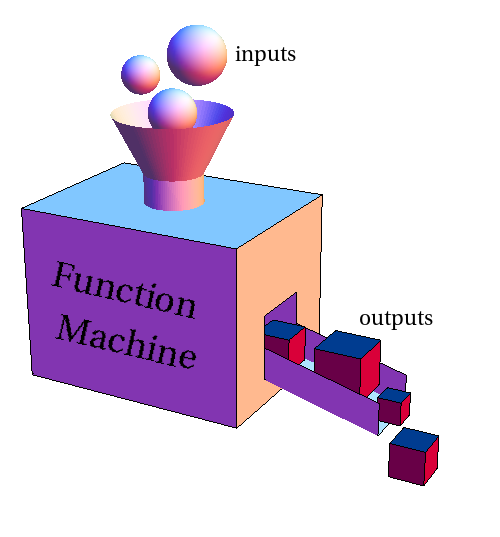
\includegraphics{images/function_machine} 

}

\caption{Ilustración de una función, tomada de www.mathinsight.org.}\label{fig:machine2}
\end{figure}

\section{\texorpdfstring{Partes de una función en \proglang{R}
\index{partes de función}}{Partes de una función en  }}\label{partes-de-una-funcion-en}

Las partes de una función son:

\begin{itemize}
\tightlist
\item
  Entradas: o llamadas también \textbf{argumentos}, sirven para ingresar
  información necesaria para realizar el procedimiento de la función.
  Los argumentos pueden estar vacíos y a la espera de que el usuario
  ingrese valores, o pueden tener valores por defecto, esto significa
  que si el usuario no ingresa una valor al función usará el valor por
  defecto. Una función puede tener o no argumentos de entrada, en los
  ejemplos se mostrarán estos casos.
\item
  Cuerpo: el cuerpo de la función está formado por un conjunto de
  instrucciones que transforman las entradas en las salidas deseadas. Si
  el cuerpo de la función está formado por varias instrucciones éstas
  deben ir entre llaves.
\item
  Salidas: son los resultados de la función. Toda función debe tener al
  menos un resultado, si una función no genera un resultado entonces no
  sirve para nada. Si una función entrega varios tipos de objetos se
  acostumbra a organizarlos en una lista que puede manejar los
  diferentes tipos de objetos.
\end{itemize}

\begin{Shaded}
\begin{Highlighting}[]
\NormalTok{nombre_de_funcion <-}\StringTok{ }\NormalTok{function(par1, par2, ...) \{}
  \NormalTok{cuerpo}
  \NormalTok{cuerpo}
  \NormalTok{cuerpo}
  \NormalTok{cuerpo}
  \KeywordTok{return}\NormalTok{(resultado)}
\NormalTok{\}}
\end{Highlighting}
\end{Shaded}

A continuación se mostrarán varios ejemplos \textbf{sencillos} para que
el lector aprenda a construir funciones.

\subsection*{Ejemplo}\label{ejemplo-15}


Construir una función que reciba dos números y que entregue la suma de
estos números.

Lo primero es elegir un nombre apropiado para la función, aquí se usó el
nombre \texttt{suma} porque así se tiene una idea clara de lo que hace
la función. La función suma recibe dos parámetros, \texttt{x} representa
el primer valor ingresado mientras que \texttt{y} representa el segundo.
El cuerpo de la función está formado por dos líneas, en la primera se
crea el objeto \texttt{resultado} en el cual se almanacena el valor de
la suma, en la segunda línea se le indica a \proglang{R} que queremos
que retorne el valor de la suma almacenada en el objeto
\texttt{resultado}. A continuación se muestra el código para crear la
función solicitada.

\begin{Shaded}
\begin{Highlighting}[]
\NormalTok{suma <-}\StringTok{ }\NormalTok{function(x, y) \{}
  \NormalTok{resultado <-}\StringTok{ }\NormalTok{x +}\StringTok{ }\NormalTok{y}
  \KeywordTok{return}\NormalTok{(resultado)}
\NormalTok{\}}
\end{Highlighting}
\end{Shaded}

Para usar la función creada sólo se debe ejecutar, vamos a obtener la
suma de los valores 4 y 6 usando la función \texttt{suma}, a
continuación el código necesario.

\begin{Shaded}
\begin{Highlighting}[]
\KeywordTok{suma}\NormalTok{(}\DataTypeTok{x=}\DecValTok{4}\NormalTok{, }\DataTypeTok{y=}\DecValTok{6}\NormalTok{)}
\end{Highlighting}
\end{Shaded}

\begin{verbatim}
## [1] 10
\end{verbatim}

Para funciones simples como la anterior es posible escribirlas en forma
más compacta. Es posible reducir el cuerpo de la función de 2 líneas a
sólo una línea solicitándole a \proglang{R} que retorne directamente la
suma sin almacenarla en ningún objeto. A continuación la función
\texttt{suma} modificada.

\begin{Shaded}
\begin{Highlighting}[]
\NormalTok{suma <-}\StringTok{ }\NormalTok{function(x, y) \{}
  \KeywordTok{return}\NormalTok{(x +}\StringTok{ }\NormalTok{y)}
\NormalTok{\}}

\KeywordTok{suma}\NormalTok{(}\DataTypeTok{x=}\DecValTok{4}\NormalTok{, }\DataTypeTok{y=}\DecValTok{6}\NormalTok{)  }\CommentTok{# Probando la función}
\end{Highlighting}
\end{Shaded}

\begin{verbatim}
## [1] 10
\end{verbatim}

Debido a que la función \texttt{suma} tiene un cuerpo muy reducido es
posible escribirla en forma más compacta, en una sola línea. A
continuación se muestra el código para reescribir la función.

\begin{Shaded}
\begin{Highlighting}[]
\NormalTok{suma <-}\StringTok{ }\NormalTok{function(x, y) x +}\StringTok{ }\NormalTok{y}

\KeywordTok{suma}\NormalTok{(}\DataTypeTok{x=}\DecValTok{4}\NormalTok{, }\DataTypeTok{y=}\DecValTok{6}\NormalTok{)  }\CommentTok{# Probando la función}
\end{Highlighting}
\end{Shaded}

\begin{verbatim}
## [1] 10
\end{verbatim}

\subsection*{Ejemplo}\label{ejemplo-16}


Construir una función que genere números aleatorios entre cero y uno
hasta que la suma de éstos números supere por primera vez el valor de 3.
La función debe entregar la cantidad de números aleatorios generados
para que se cumpla la condición.

Vamos a llamar la función solicitada con el nombre \texttt{fun1}, esta
función \textbf{NO} necesita ningún parámetro de entrada. El valor de 3
que está en la condición puede ir dentro del cuerpo y por eso no se
necesitan parámetros para esta función. En el cuerpo de la función se
genera un vector con un número aleatorio y luego se chequea si la suma
de sus elementos es menor de 3, si se cumple que la suma es menor que 3
se siguen generando números que se almacenan en el vector \texttt{num}.
Una vez que la suma exceda el valor de 3 NO se ingresa al \texttt{while}
y se pide la longitud del vector o el valor de \texttt{veces}
solicitado. A continuación el código de la función.

\begin{Shaded}
\begin{Highlighting}[]
\NormalTok{fun1 <-}\StringTok{ }\NormalTok{function() \{}
  \NormalTok{num <-}\StringTok{ }\KeywordTok{runif}\NormalTok{(}\DecValTok{1}\NormalTok{)}
  \NormalTok{veces <-}\StringTok{ }\DecValTok{1}
  \NormalTok{while (}\KeywordTok{sum}\NormalTok{(num) <}\StringTok{ }\DecValTok{3}\NormalTok{) \{}
    \NormalTok{veces <-}\StringTok{ }\NormalTok{veces +}\StringTok{ }\DecValTok{1}
    \NormalTok{num[veces] <-}\StringTok{ }\KeywordTok{runif}\NormalTok{(}\DecValTok{1}\NormalTok{)}
  \NormalTok{\}}
  \KeywordTok{return}\NormalTok{(veces)}
\NormalTok{\}}

\KeywordTok{fun1}\NormalTok{()  }\CommentTok{# primera prueba}
\end{Highlighting}
\end{Shaded}

\begin{verbatim}
## [1] 8
\end{verbatim}

\subsection*{Ejemplo}\label{ejemplo-17}


Construir una función que, dado un número entero positivo (cota)
ingresado por el usuario, genere números aleatorios entre cero y uno
hasta que la suma de los números generados exceda por primera vez la
cota. La función debe entregar un vector con los números aleatorios, la
suma y la cantidad de números aleatorios. Si el usuario no ingresa el
valor de la cota, se debe asumir igual a 1.

La función aquí solicitada es similar a la construída en el ejemplo
anterior. La función \texttt{fun2} tiene un sólo parámetro con el valor
por defecto, si el usuario no ingresa valor a este parámetro, se asumirá
el valor de uno. El cuerpo de la función es similar al anterior. Como la
función debe entregar un vector y dos números, se construye la lista
\texttt{resultado} que almacena los tres objetos solicitados. A
continuación el código para función solicitada.

\begin{Shaded}
\begin{Highlighting}[]
\NormalTok{fun2 <-}\StringTok{ }\NormalTok{function(}\DataTypeTok{cota=}\DecValTok{1}\NormalTok{) \{}
  \NormalTok{num <-}\StringTok{ }\KeywordTok{runif}\NormalTok{(}\DecValTok{1}\NormalTok{)}
  \NormalTok{while (}\KeywordTok{sum}\NormalTok{(num) <}\StringTok{ }\NormalTok{cota) \{}
    \NormalTok{num <-}\StringTok{ }\KeywordTok{c}\NormalTok{(num, }\KeywordTok{runif}\NormalTok{(}\DecValTok{1}\NormalTok{))}
  \NormalTok{\}}
  \NormalTok{resultado <-}\StringTok{ }\KeywordTok{list}\NormalTok{(}\DataTypeTok{vector=}\NormalTok{num,}
                    \DataTypeTok{suma=}\KeywordTok{sum}\NormalTok{(num),}
                    \DataTypeTok{cantidad=}\KeywordTok{length}\NormalTok{(num))}
  \KeywordTok{return}\NormalTok{(resultado)}
\NormalTok{\}}
\end{Highlighting}
\end{Shaded}

Probando la función con cota de uno.

\begin{Shaded}
\begin{Highlighting}[]
\KeywordTok{fun2}\NormalTok{()}
\end{Highlighting}
\end{Shaded}

\begin{verbatim}
## $vector
## [1] 0.001137 0.391203 0.462495 0.388144
## 
## $suma
## [1] 1.243
## 
## $cantidad
## [1] 4
\end{verbatim}

Probando la función con cota de tres.

\begin{Shaded}
\begin{Highlighting}[]
\KeywordTok{fun2}\NormalTok{(}\DataTypeTok{cota=}\DecValTok{3}\NormalTok{)}
\end{Highlighting}
\end{Shaded}

\begin{verbatim}
## $vector
## [1] 0.4025 0.1790 0.9517 0.4537 0.3268 0.9654
## 
## $suma
## [1] 3.279
## 
## $cantidad
## [1] 6
\end{verbatim}

\subsection*{Ejemplo}\label{ejemplo-18}


Construya una función que reciba dos números de la recta real y que
entregue el punto médio de estos números. El resultado debe ser un
mensaje por pantalla.

El punto médio entre dos valores es la suma de los números divido entre
dos. La función \texttt{cat} sirve para concatenar objetos y
presentarlos por pantalla. A continuación el código para la función
requerida.

\begin{Shaded}
\begin{Highlighting}[]
\NormalTok{medio <-}\StringTok{ }\NormalTok{function(a, b) \{}
  \NormalTok{medio <-}\StringTok{ }\NormalTok{(a +}\StringTok{ }\NormalTok{b) /}\StringTok{ }\DecValTok{2}
  \KeywordTok{cat}\NormalTok{(}\StringTok{"El punto medio de los valores"}\NormalTok{,}
      \NormalTok{a, }\StringTok{"y"}\NormalTok{, b,}
      \StringTok{"ingresados es"}\NormalTok{, medio)}
\NormalTok{\}}

\KeywordTok{medio}\NormalTok{(}\DataTypeTok{a=}\NormalTok{-}\DecValTok{3}\NormalTok{, }\DataTypeTok{b=}\NormalTok{-}\DecValTok{1}\NormalTok{)  }\CommentTok{# Probando la función}
\end{Highlighting}
\end{Shaded}

\begin{verbatim}
## El punto medio de los valores -3 y -1 ingresados es -2
\end{verbatim}

\BeginKnitrBlock{rmdnote}
La función \texttt{cat} es muy útil para presentar resultados por
pantalla. Consulte la ayuda de la función para ver otros ejemplos.
\EndKnitrBlock{rmdnote}

\section*{EJERCICIOS}\label{ejercicios-2}


Construir funciones en \proglang{R} que realicen lo solicitado.

\begin{enumerate}
\def\labelenumi{\arabic{enumi}.}
\item
  Construya una función que reciba dos números reales y que diga cuál es
  el mayor de ellos.
\item
  Escriba una función llamada media que calcule la media muestral de un
  vector numérico ingresado a la función. A continuación la fórmula para
  calcular la media muestral.
\end{enumerate}

\[\bar{x}=\frac{\sum_{i=1}^n x_i}{n}\] Verifique el desempeño de su
función comparando con la función \texttt{mean}. Corra el siguiente
código para hacer la prueba, los resultados deben coincidir.

\begin{Shaded}
\begin{Highlighting}[]
\NormalTok{x <-}\StringTok{ }\KeywordTok{runif}\NormalTok{(}\DataTypeTok{n=}\DecValTok{100}\NormalTok{)}
\KeywordTok{media}\NormalTok{(x)}
\KeywordTok{mean}\NormalTok{(x)}
\end{Highlighting}
\end{Shaded}

\begin{enumerate}
\def\labelenumi{\arabic{enumi}.}
\setcounter{enumi}{2}
\item
  Construya una función que encuentre las raíces de una ecuación de
  segundo grado. El usuario debe suministrar los coeficientes
  \texttt{a}, \texttt{b} y \texttt{c} de la ecuación \(ax^2+bx+c=0\) y
  la función debe entregar las raíces.
\item
  Escribir una función que calcule la velocidad de un proyectil dado que
  el usuario ingresa la distancia Km y el tiempo en minutos. Expresar el
  resultado en metros/segundo, recuerde que
  \(velocidad = espacio / tiempo\).
\end{enumerate}

\chapter{\texorpdfstring{Lectura de bases de datos
\index{lectura de bases de datos}}{Lectura de bases de datos }}\label{lectura-de-bases-de-datos}

En este capítulo se mostrará cómo leer una base de datos externa hacia
\proglang{R}.

\section{\texorpdfstring{¿En qué formato almacenar una base de datos?
\index{.csv}
\index{.txt}}{¿En qué formato almacenar una base de datos?  }}\label{en-que-formato-almacenar-una-base-de-datos}

Usualmente los archivos con la información para ser leídos por
\proglang{R} se pueden almacenar en formato:

\begin{itemize}
\tightlist
\item
  plano con extensión \textbf{.txt} o,
\item
  Excel con extensión \textbf{.csv}.
\end{itemize}

En las secciones siguientes se mostrará cómo almacenar datos en los dos
formatos para ser leídos en \proglang{R}. En el Cuadro \ref{tab:dt1} se
presenta una base de datos pequeña, tres observaciones y tres variables,
que nos servirá como ejemplo para mostrar cómo se debe almacenar la
información.

\begin{table}

\caption{\label{tab:dt1}Ejemplo de una base de datos simple.}
\centering
\begin{tabular}[t]{rll}
\toprule
Edad & Fuma & Pais\\
\midrule
35 & TRUE & Colombia\\
46 & TRUE & Francia\\
23 & FALSE & Malta\\
\bottomrule
\end{tabular}
\end{table}

\subsection{\texorpdfstring{Almacenamiento de información en Excel
\index{Excel}}{Almacenamiento de información en Excel }}\label{almacenamiento-de-informacion-en-excel}

Para almacenar la información del Cuadro \ref{tab:dt1} en Excel, abrimos
un archivo nuevo archivo de Excel y copiamos la información tal como se
muestra en la Figura \ref{fig:excel1}. Se debe iniciar en la parte
superior izquierda, no se deben dejar filas vacías, no se debe colorear,
no se deben colocar bordes ni nada, se ingresa la información sin
embellecer el contenido. Por último se guarda el archivo en la carpeta
deseada y al momento de nombrar el archivo se debe modificar la opción
tipo de archivo a \textbf{csv (delimitado por comas)}.

\begin{figure}

{\centering 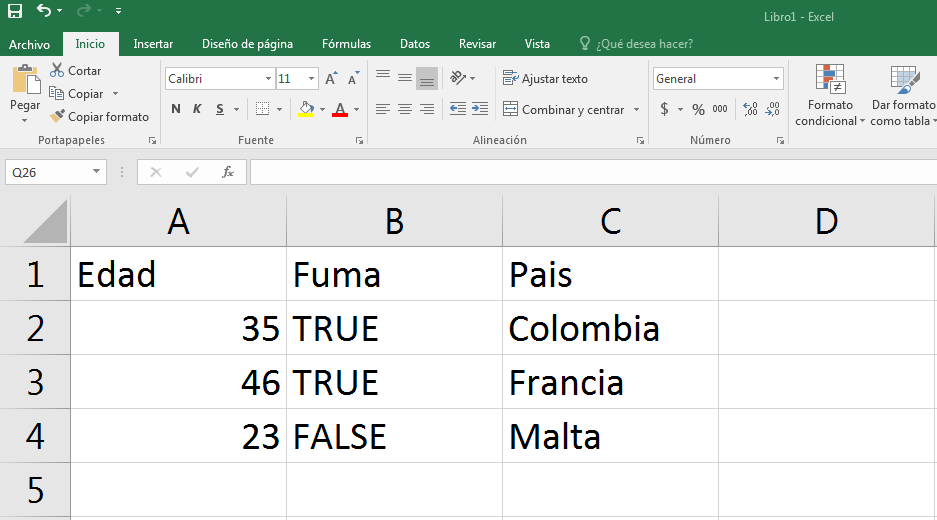
\includegraphics{images/excel1} 

}

\caption{Forma de almacenar los datos en Excel.}\label{fig:excel1}
\end{figure}

\BeginKnitrBlock{rmdwarning}
Recuerde que el archivo de Excel se debe guardar con extensión .csv.
\EndKnitrBlock{rmdwarning}

\subsection{\texorpdfstring{Almacenamiento de información en bloc de
notas
\index{bloc de notas}}{Almacenamiento de información en bloc de notas }}\label{almacenamiento-de-informacion-en-bloc-de-notas}

Para almacenar la información del Cuadro \ref{tab:dt1} en bloc de notas,
abrimos un archivo nuevo de bloc de notas y copiamos la información tal
como se muestra en la Figura \ref{fig:bloc1}. Se copian los nombres de
las variables o los datos separados por un espacio obtenido con la tecla
tabuladora, cada línea se finaliza con un \emph{enter}. Se recomienda al
guardar el archivo que el cursor al inicio de una línea vacía, en la
Figura \ref{fig:bloc1} se señala la posición del cursor con la flecha
roja, a pesar de que no éxiste línea número 5, el curso debe quedar al
inicio de esa línea número 5.

\begin{figure}

{\centering 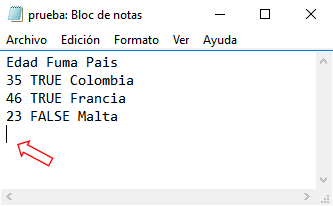
\includegraphics{images/bloc1} 

}

\caption{Almacenamiento de los datos en bloc de notas usando la barra espaciadora}\label{fig:bloc1}
\end{figure}

Es posible mejorar la apariencia de la información almacenada en el bloc
de notas si, en lugar de usar espacios con la barra espaciadora, se
colocan los espacios con la barra tabuladora, así la información se ve
más organizada y se puede chequear fácilmente la información ingresada.
En la Figura \ref{fig:bloc2} se muestra la información para el ejemplo,
claramente se nota la organización de la información.

\begin{figure}

{\centering 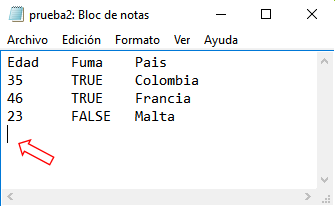
\includegraphics{images/bloc2} 

}

\caption{Almacenamiento de los datos en bloc de notas usando la barra tabuladora}\label{fig:bloc2}
\end{figure}

\BeginKnitrBlock{rmdtip}
Una buena práctica es usar la barra tabuladora para separar, eso permite
que la información se vea ordenada.
\EndKnitrBlock{rmdtip}

\section{\texorpdfstring{Función \texttt{read.table}
\index{read.table}}{Función read.table }}\label{funcion-read.table}

La función \texttt{read.table} se puede usar para leer bases de datos
hacia \proglang{R}. La estructura de la función con los parámetros más
comunes de uso es la siguiente.

\begin{Shaded}
\begin{Highlighting}[]
\KeywordTok{read.table}\NormalTok{(file, header, sep, dec)}
\end{Highlighting}
\end{Shaded}

Los argumentos de la función \texttt{read.table} son:

\begin{itemize}
\tightlist
\item
  \texttt{file}: nombre o ruta donde están alojados los datos. Puede ser
  un url o una dirección del computador. Es también posible usar
  \texttt{file.choose()} para que se abra un ventana y adjuntar el
  archivo deseado manualmente.
\item
  \texttt{header}: valor lógico, se usa \texttt{TRUE} si la primera
  línea de la base de datos tiene los nombres de las variables, caso
  contrario se usa \texttt{FALSE}.
\item
  \texttt{sep}: tipo de separación interna para los datos dentro del
  archivo. Los valores usuales para este parámetros son:

  \begin{itemize}
  \tightlist
  \item
    \texttt{sep=\textquotesingle{},\textquotesingle{}} si el archivo
    tiene extensión .csv.
  \item
    \texttt{sep=\textquotesingle{}\textquotesingle{}} si el archivo es
    bloc de notas con espacios por la barra \textbf{espaciadora}.
  \item
    \texttt{sep=\textquotesingle{}\textbackslash{}t\textquotesingle{}}
    si el archivo es bloc de notas con espacios por la barra
    \textbf{tabuladora}.
  \end{itemize}
\item
  \texttt{dec}: símbolo con el cual están indicados los decimales.
\end{itemize}

\subsection*{Ejemplo}\label{ejemplo-19}


Crear la base de datos del Cuadro \ref{tab:dt1} en Excel y bloc de notas
para practicar la lectura de base de datos desde \proglang{R}.

Lo primero que se debe hacer para realizar lo solicitado es construir
tres archivos (uno de Excel y dos bloc de notas) igual a los mostrados
en las figuras \ref{fig:excel1}, \ref{fig:bloc1} y \ref{fig:bloc2},
vamos a suponer que los nombres para cada uno de ellos son
\texttt{base1.csv}, \texttt{base2.txt} y \texttt{base3.txt}
respectivamente.

\subsubsection*{Para Excel}\label{para-excel}


Para leer el archivo de Excel llamado \texttt{base1.csv} podemos usar el
siguiente código.

\begin{Shaded}
\begin{Highlighting}[]
\NormalTok{datos <-}\StringTok{ }\KeywordTok{read.table}\NormalTok{(}\DataTypeTok{file=}\StringTok{'C:/Users/Hernandez/Desktop/base1.csv'}\NormalTok{,}
                    \DataTypeTok{header=}\OtherTok{TRUE}\NormalTok{, }\DataTypeTok{sep=}\StringTok{','}\NormalTok{)}
\NormalTok{datos}
\end{Highlighting}
\end{Shaded}

La dirección
\texttt{file=\textquotesingle{}C:/Users/Hernandez/Desktop/base1.csv\textquotesingle{}}
le indica a \proglang{R} en qué lugar del computador debe buscar el
archivo, note que se debe usar el símbolo \texttt{/} para que sea un
dirección válida. Substituya la dirección del código anterior con la
dirección donde se encuentra su archivo para que pueda leer la base de
datos.

Si no se conoce la ubicación del archivo a leer o si la dirección es muy
extensa, se puede usar \texttt{file.choose()} para que se abra una
ventana y así adjuntar manualmente el archivo. A continuación se muestra
el código para hacerlo de esta manera.

\begin{Shaded}
\begin{Highlighting}[]
\NormalTok{datos <-}\StringTok{ }\KeywordTok{read.table}\NormalTok{(}\KeywordTok{file.choose}\NormalTok{(), }\DataTypeTok{header=}\OtherTok{TRUE}\NormalTok{, }\DataTypeTok{sep=}\StringTok{','}\NormalTok{)}
\NormalTok{datos}
\end{Highlighting}
\end{Shaded}

\subsubsection*{Para bloc de notas con barra
espaciadora}\label{para-bloc-de-notas-con-barra-espaciadora}
\addcontentsline{toc}{subsubsection}{Para bloc de notas con barra
espaciadora}

Para leer el archivo de Excel llamado \texttt{base2.txt} podemos usar el
siguiente código.

\begin{Shaded}
\begin{Highlighting}[]
\NormalTok{datos <-}\StringTok{ }\KeywordTok{read.table}\NormalTok{(}\DataTypeTok{file=}\StringTok{'C:/Users/Hernandez/Desktop/base2.txt'}\NormalTok{,}
                    \DataTypeTok{header=}\OtherTok{TRUE}\NormalTok{, }\DataTypeTok{sep=}\StringTok{''}\NormalTok{)}
\NormalTok{datos}
\end{Highlighting}
\end{Shaded}

\subsubsection*{Para bloc de notas con barra
tabuladora}\label{para-bloc-de-notas-con-barra-tabuladora}
\addcontentsline{toc}{subsubsection}{Para bloc de notas con barra
tabuladora}

Para leer el archivo de Excel llamado \texttt{base3.txt} podemos usar el
siguiente código.

\begin{Shaded}
\begin{Highlighting}[]
\NormalTok{datos <-}\StringTok{ }\KeywordTok{read.table}\NormalTok{(}\DataTypeTok{file=}\StringTok{'C:/Users/Hernandez/Desktop/base3.txt'}\NormalTok{,}
                    \DataTypeTok{header=}\OtherTok{TRUE}\NormalTok{, }\DataTypeTok{sep=}\StringTok{'}\CharTok{\textbackslash{}t}\StringTok{'}\NormalTok{)}
\NormalTok{datos}
\end{Highlighting}
\end{Shaded}

\BeginKnitrBlock{rmdnote}
El usuario puede usar indiferentemente
\texttt{file=\textquotesingle{}C:/Users/bla/bla\textquotesingle{}} o
\texttt{file.choose()} para ingresar el archivo, con la práctica se
aprende a decidir cuando conviene una u otra forma.
\EndKnitrBlock{rmdnote}

\BeginKnitrBlock{rmdwarning}
Un error frecuente es escribir la dirección o ubicación del archivo
usando \texttt{\textbackslash{}}, lo correcto es usar \texttt{/}.
\EndKnitrBlock{rmdwarning}

\subsection*{Ejemplo}\label{ejemplo-20}


Leer la base de datos sobre apartamentos usados en la ciudad de Medellín
que está disponible en la página web cuya url es:
\url{https://raw.githubusercontent.com/fhernanb/datos/master/aptos2015}

Para leer la base de datos desde una url usamos el siguiente código.

\begin{Shaded}
\begin{Highlighting}[]
\NormalTok{enlace <-}\StringTok{ 'https://raw.githubusercontent.com/fhernanb/datos/master/aptos2015'}
\NormalTok{datos <-}\StringTok{ }\KeywordTok{read.table}\NormalTok{(}\DataTypeTok{file=}\NormalTok{enlace, }\DataTypeTok{header=}\OtherTok{TRUE}\NormalTok{)}
\end{Highlighting}
\end{Shaded}

La base de datos ingresada queda en el marco de datos llamado
\texttt{datos} y ya está disponible para usarla.

\section{Lectura de bases de datos en
Excel}\label{lectura-de-bases-de-datos-en-excel}

Algunas veces los datos están disponibles en un archivo estándar de
Excel, y dentro de cada archivo hojas con la información a utilizar. En
estos casos se recomienda usar el paquete \textbf{readxl}\index{readxl}
\citep{R-readxl} y en particular la función \texttt{readxl}. A
continuación un ejemplo de cómo proceder en estos casos.

\subsection*{Ejemplo}\label{ejemplo-21}


En este
\href{https://github.com/fhernanb/datos/blob/master/BD_Excel.xlsx}{enlace}
está disponible un archivo de Excel llamado BD\_Excel.xlxs, una vez se
ha abierto la página donde está alojado el archivo, se debe descargar y
guardar en alguna carpeta. El archivo contiene dos bases de datos muy
pequeñas, en la primera hoja llamada \textbf{Hijos} está la información
de un grupo de niños y en la segunda hoja llamada \textbf{Padres} está
la información de los padres. ¿Cómo se pueden leer las dos bases de
datos?

Lo primero que se debe hacer es instalar el paquete \textbf{readxl}, la
instalación de cualquier paquete en un computador se hace una sola vez y
éste quedará instalado para ser usado las veces que se requiera. La
función para instalar un paquete cualquiera es
\texttt{install.packages}, a continuación se muestra el código necesario
para instalar el paquete \textbf{readxl}.

\begin{Shaded}
\begin{Highlighting}[]
\KeywordTok{install.packages}\NormalTok{(}\StringTok{"readxl"}\NormalTok{)}
\end{Highlighting}
\end{Shaded}

Una vez instalado el paquete es necesario cargarlo, la función para
cargar el paquete en la sesión actual de \proglang{R} es
\texttt{library}. La instrucción para cargar el paquete es la siguiente:

\begin{Shaded}
\begin{Highlighting}[]
\KeywordTok{library}\NormalTok{(readxl)}
\end{Highlighting}
\end{Shaded}

\BeginKnitrBlock{rmdwarning}
La instalación de un paquete con \texttt{install.packages} se hace sólo
una vez y no más. Cargar el paquete con \texttt{library} en la sesión
actual se debe hacer siempre que se vaya a usar el paquete.
\EndKnitrBlock{rmdwarning}

Luego de haber cargado el paquete \textbf{readxl} se puede usar la
función \texttt{readxl} para leer la información contenida en las hojas.
A continuación el código para crear la base de datos \texttt{hijos}
contenida en el archivo BD\_Excel.xlsx.

\begin{Shaded}
\begin{Highlighting}[]
\NormalTok{hijos <-}\StringTok{ }\KeywordTok{read_excel}\NormalTok{(}\KeywordTok{file.choose}\NormalTok{(), }\DataTypeTok{sheet=}\StringTok{'Hijos'}\NormalTok{)}
\NormalTok{hijos  }\CommentTok{# Para ver el contenido}
\end{Highlighting}
\end{Shaded}

\begin{verbatim}
##   Edad Grado    ComicFav
## 1    8     2    Superman
## 2    6     1      Batman
## 3    9     3      Batman
## 4   10     5 Bob Esponja
## 5    8     4      Batman
## 6    9     4 Bob Esponja
\end{verbatim}

A continuación el código para crear la base de datos \texttt{padres}
contenida en el archivo BD\_Excel.xlsx.

\begin{Shaded}
\begin{Highlighting}[]
\NormalTok{padres <-}\StringTok{ }\KeywordTok{read_excel}\NormalTok{(}\StringTok{'BD_Excel.xlsx'}\NormalTok{, }\DataTypeTok{sheet=}\StringTok{'Padres'}\NormalTok{)}
\NormalTok{padres  }\CommentTok{# Para ver el contenido}
\end{Highlighting}
\end{Shaded}

\begin{verbatim}
##   Edad   EstCivil NumHijos
## 1   45    Soltero        1
## 2   50     Casado        0
## 3   35     Casado        3
## 4   65 Divorciado        1
\end{verbatim}

La función \texttt{readxl} tiene otros parámetros adicionales útiles
para leer bases de datos, se recomienda consultar la ayuda de la función
escribiendo en la consola \texttt{help(read.xl)}.

\section*{EJERCICIOS}\label{ejercicios-3}


Realice los siguiente ejercicios propuestos.

\begin{enumerate}
\def\labelenumi{\arabic{enumi}.}
\tightlist
\item
  En el Cuadro \ref{tab:toy} se presenta una base de datos sencilla.
  Almacene la información del cuadro en dos archivos diferentes, en
  Excel y en bloc de notas. Lea los dos archivos con la función
  \texttt{read.table} y compare los resultados obtenidos con la del
  Cuadro \ref{tab:toy} fuente.
\end{enumerate}

\begin{table}

\caption{\label{tab:toy}Base de datos para practicar lectura.}
\centering
\begin{tabular}[t]{llrr}
\toprule
Fuma & Pasatiempo & Num\_hermanos & Mesada\\
\midrule
Si & Lectura & 0 & 4500\\
Si & NA & 2 & 2600\\
No & Correr & 4 & 1000\\
No & Correr & NA & 3990\\
Si & TV & 3 & 2570\\
\addlinespace
No & TV & 1 & 2371\\
Si & Correr & 1 & 1389\\
NA & Correr & 0 & 4589\\
Si & Lectura & 2 & NA\\
\bottomrule
\end{tabular}
\end{table}

\begin{enumerate}
\def\labelenumi{\arabic{enumi}.}
\setcounter{enumi}{1}
\tightlist
\item
  En la url
  \url{https://raw.githubusercontent.com/fhernanb/datos/master/medidas_cuerpo}
  están disponibles los datos sobre medidas corporales para un grupo de
  estudiante de la universidad, use la función \texttt{read.table} para
  leer la base de datos.
\end{enumerate}

\chapter{\texorpdfstring{Tablas de frecuencia
\index{tablas de frecuencia}}{Tablas de frecuencia }}\label{tablas-de-frecuencia}

Las tablas de frecuencia son muy utilizadas en estadística y
\proglang{R} permite crear tablas de una forma sencilla. En este
capítulo se explican las principales funciones para la elaboración de
tablas.

\section{\texorpdfstring{Tabla de contingencia con \texttt{table}
\index{table}}{Tabla de contingencia con table }}\label{tabla-de-contingencia-con-table}

La función \texttt{table} sirve para construir tablas de frecuencia de
una vía, a continuación la estrctura de la función.

\begin{Shaded}
\begin{Highlighting}[]
\KeywordTok{table}\NormalTok{(..., exclude, useNA)}
\end{Highlighting}
\end{Shaded}

Los parámetros de la función son:

\begin{itemize}
\tightlist
\item
  \texttt{...} espacio para ubicar los nombres de los objetos (variables
  o vectores) para los cuales se quiere construir la tabla.
\item
  \texttt{exclude}: vector con los niveles a remover de la tabla. Si
  \texttt{exclude=NULL} implica que se desean ver los \texttt{NA}, lo
  que equivale a
  \texttt{useNA\ =\ \textquotesingle{}always\textquotesingle{}}.
\item
  \texttt{useNA}: instrucción de lo que se desea con los \texttt{NA}.
  Hay tres posibles valores para este parámetro:
  \texttt{\textquotesingle{}no\textquotesingle{}} si no se desean usar,
  \texttt{\textquotesingle{}ifany\textquotesingle{}} y
  \texttt{\textquotesingle{}always\textquotesingle{}} si se desean
  incluir.
\end{itemize}

\subsection*{Ejemplo: tabla de frecuencia de una
vía}\label{ejemplo-tabla-de-frecuencia-de-una-via}
\addcontentsline{toc}{subsection}{Ejemplo: tabla de frecuencia de una
vía}

Considere el vector \texttt{fuma} mostrado a continuación y construya
una tabla de frecuencias absolutas para los niveles de la variable
frecuencia de fumar.

\begin{Shaded}
\begin{Highlighting}[]
\NormalTok{fuma <-}\StringTok{ }\KeywordTok{c}\NormalTok{(}\StringTok{'Frecuente'}\NormalTok{, }\StringTok{'Nunca'}\NormalTok{, }\StringTok{'A veces'}\NormalTok{, }\StringTok{'A veces'}\NormalTok{, }\StringTok{'A veces'}\NormalTok{,}
          \StringTok{'Nunca'}\NormalTok{, }\StringTok{'Frecuente'}\NormalTok{, }\OtherTok{NA}\NormalTok{, }\StringTok{'Frecuente'}\NormalTok{, }\OtherTok{NA}\NormalTok{, }\StringTok{'hola'}\NormalTok{, }
          \StringTok{'Nunca'}\NormalTok{, }\StringTok{'Hola'}\NormalTok{, }\StringTok{'Frecuente'}\NormalTok{, }\StringTok{'Nunca'}\NormalTok{)}
\end{Highlighting}
\end{Shaded}

A continuación se muestra el código para crear la tabla de frecuencias
para la variable \texttt{fuma}.

\begin{Shaded}
\begin{Highlighting}[]
\KeywordTok{table}\NormalTok{(fuma)}
\end{Highlighting}
\end{Shaded}

\begin{verbatim}
## fuma
##   A veces Frecuente      hola      Hola     Nunca 
##         3         4         1         1         4
\end{verbatim}

De la tabla anterior vemos que NO aparece el conteo de los \texttt{NA},
para obtenerlo usamos lo siguiente.

\begin{Shaded}
\begin{Highlighting}[]
\KeywordTok{table}\NormalTok{(fuma, }\DataTypeTok{useNA=}\StringTok{'always'}\NormalTok{)}
\end{Highlighting}
\end{Shaded}

\begin{verbatim}
## fuma
##   A veces Frecuente      hola      Hola     Nunca 
##         3         4         1         1         4 
##      <NA> 
##         2
\end{verbatim}

Vemos que hay dos niveles errados en la tabla anterior, \texttt{Hola} y
\texttt{hola}. Para construir la tabla sin esos niveles errados usamos
lo siguiente.

\begin{Shaded}
\begin{Highlighting}[]
\KeywordTok{table}\NormalTok{(fuma, }\DataTypeTok{exclude=}\KeywordTok{c}\NormalTok{(}\StringTok{'Hola'}\NormalTok{, }\StringTok{'hola'}\NormalTok{))}
\end{Highlighting}
\end{Shaded}

\begin{verbatim}
## fuma
##   A veces Frecuente     Nunca      <NA> 
##         3         4         4         2
\end{verbatim}

Por último construyamos la tabla sin los niveles errados y los
\texttt{NA}, a esta última tabla la llamaremos \texttt{tabla1} para
luego poder usarla. Las instrucciones para hacer esto son las
siguientes.

\begin{Shaded}
\begin{Highlighting}[]
\NormalTok{tabla1 <-}\StringTok{ }\KeywordTok{table}\NormalTok{(fuma, }\DataTypeTok{exclude=}\KeywordTok{c}\NormalTok{(}\StringTok{'Hola'}\NormalTok{, }\StringTok{'hola'}\NormalTok{, }\OtherTok{NA}\NormalTok{))}
\NormalTok{tabla1}
\end{Highlighting}
\end{Shaded}

\begin{verbatim}
## fuma
##   A veces Frecuente     Nunca 
##         3         4         4
\end{verbatim}

\BeginKnitrBlock{rmdnote}
Al crear una tabla con la instrucción \texttt{table(var1,\ var2)}, la
variable 1 quedará por filas mientras que la variable 2 estará en las
columnas.
\EndKnitrBlock{rmdnote}

\subsection*{Ejemplo: tabla de frecuencia de dos
vías}\label{ejemplo-tabla-de-frecuencia-de-dos-vias}
\addcontentsline{toc}{subsection}{Ejemplo: tabla de frecuencia de dos
vías}

Considere otro vector \texttt{sexo} mostrado a continuación y construya
una tabla de frecuencias absolutas para ver cómo se relaciona el sexo
con fumar del ejemplo anterior.

\begin{Shaded}
\begin{Highlighting}[]
\NormalTok{sexo <-}\StringTok{ }\KeywordTok{c}\NormalTok{(}\StringTok{'Hombre'}\NormalTok{, }\StringTok{'Hombre'}\NormalTok{, }\StringTok{'Hombre'}\NormalTok{, }\OtherTok{NA}\NormalTok{, }\StringTok{'Mujer'}\NormalTok{,}
          \StringTok{'Casa'}\NormalTok{, }\StringTok{'Mujer'}\NormalTok{, }\StringTok{'Mujer'}\NormalTok{, }\StringTok{'Mujer'}\NormalTok{, }\StringTok{'Hombre'}\NormalTok{, }\StringTok{'Mujer'}\NormalTok{, }
          \StringTok{'Hombre'}\NormalTok{, }\OtherTok{NA}\NormalTok{, }\StringTok{'Mujer'}\NormalTok{, }\StringTok{'Mujer'}\NormalTok{)}
\end{Highlighting}
\end{Shaded}

Para construir la tabla solicitada usamos el siguiente código.

\begin{Shaded}
\begin{Highlighting}[]
\KeywordTok{table}\NormalTok{(sexo, fuma)}
\end{Highlighting}
\end{Shaded}

\begin{verbatim}
##         fuma
## sexo     A veces Frecuente hola Hola Nunca
##   Casa         0         0    0    0     1
##   Hombre       1         1    0    0     2
##   Mujer        1         3    1    0     1
\end{verbatim}

De la tabla anterior vemos que aparecen niveles errados en fuma y en
sexo, para retirarlos usamos el siguiente código incluyendo en el
parámetro \texttt{exclude} un vector con los niveles que \textbf{NO}
deseamos en la tabla.

\begin{Shaded}
\begin{Highlighting}[]
\NormalTok{tabla2 <-}\StringTok{ }\KeywordTok{table}\NormalTok{(sexo, fuma, }\DataTypeTok{exclude=}\KeywordTok{c}\NormalTok{(}\StringTok{'Hola'}\NormalTok{, }\StringTok{'hola'}\NormalTok{, }\StringTok{'Casa'}\NormalTok{, }\OtherTok{NA}\NormalTok{))}
\NormalTok{tabla2}
\end{Highlighting}
\end{Shaded}

\begin{verbatim}
##         fuma
## sexo     A veces Frecuente Nunca
##   Hombre       1         1     2
##   Mujer        1         3     1
\end{verbatim}

\section{\texorpdfstring{Función \texttt{prop.table}
\index{prop.table}}{Función prop.table }}\label{funcion-prop.table}

La función \texttt{prop.table} se utiliza para crear tablas de
frecuencia relativa a partir de tablas de frecuencia absoluta, la
estructura de la función se muestra a continuación.

\begin{Shaded}
\begin{Highlighting}[]
\KeywordTok{prop.table}\NormalTok{(x, }\DataTypeTok{margin=}\OtherTok{NULL}\NormalTok{)}
\end{Highlighting}
\end{Shaded}

\begin{itemize}
\tightlist
\item
  \texttt{x}: tabla de frecuencia.
\item
  \texttt{margin}: valor de 1 si se desean proporciones por filas, 2 si
  se desean por columnas, \texttt{NULL} si se desean frecuencias
  globales.
\end{itemize}

\subsection*{Ejemplo: tabla de frecuencia relativa de una
vía}\label{ejemplo-tabla-de-frecuencia-relativa-de-una-via}
\addcontentsline{toc}{subsection}{Ejemplo: tabla de frecuencia relativa
de una vía}

Obtener la tabla de frencuencia relativa para la \texttt{tabla1}.

Para obtener la tabla solicitada se usa el siguiente código.

\begin{Shaded}
\begin{Highlighting}[]
\KeywordTok{prop.table}\NormalTok{(}\DataTypeTok{x=}\NormalTok{tabla1)}
\end{Highlighting}
\end{Shaded}

\begin{verbatim}
## fuma
##   A veces Frecuente     Nunca 
##    0.2727    0.3636    0.3636
\end{verbatim}

\subsection*{Ejemplo: tabla de frecuencia relativa de dos
vías}\label{ejemplo-tabla-de-frecuencia-relativa-de-dos-vias}
\addcontentsline{toc}{subsection}{Ejemplo: tabla de frecuencia relativa
de dos vías}

Obtener la tabla de frencuencia relativa para la \texttt{tabla2}.

Si se desea la tabla de frecuencias relativas global se usa el siguiente
código. El resultado se almacena en el objeto \texttt{tabla3} para ser
usado luego.

\begin{Shaded}
\begin{Highlighting}[]
\NormalTok{tabla3 <-}\StringTok{ }\KeywordTok{prop.table}\NormalTok{(}\DataTypeTok{x=}\NormalTok{tabla2)}
\NormalTok{tabla3}
\end{Highlighting}
\end{Shaded}

\begin{verbatim}
##         fuma
## sexo     A veces Frecuente  Nunca
##   Hombre  0.1111    0.1111 0.2222
##   Mujer   0.1111    0.3333 0.1111
\end{verbatim}

Si se desea la tabla de frecuencias relativas marginal por
\textbf{columnas} se usa el siguiente código.

\begin{Shaded}
\begin{Highlighting}[]
\NormalTok{tabla4 <-}\StringTok{ }\KeywordTok{prop.table}\NormalTok{(}\DataTypeTok{x=}\NormalTok{tabla2, }\DataTypeTok{margin=}\DecValTok{2}\NormalTok{)}
\NormalTok{tabla4}
\end{Highlighting}
\end{Shaded}

\begin{verbatim}
##         fuma
## sexo     A veces Frecuente  Nunca
##   Hombre  0.5000    0.2500 0.6667
##   Mujer   0.5000    0.7500 0.3333
\end{verbatim}

\section{\texorpdfstring{Función \texttt{addmargins}
\index{addmargins}}{Función addmargins }}\label{funcion-addmargins}

Esta función se puede utilizar para agregar los totales por filas o por
columnas a una tabla de frecuencia absoluta o relativa. La estructura de
la función es la siguiente.

\begin{Shaded}
\begin{Highlighting}[]
\KeywordTok{addmargins}\NormalTok{(A, margin)}
\end{Highlighting}
\end{Shaded}

\begin{itemize}
\tightlist
\item
  \texttt{A}: tabla de frecuencia.
\item
  \texttt{margin}: valor de 1 si se desean proporciones por columnas, 2
  si se desean por filas, \texttt{NULL} si se desean frecuencias
  globales.
\end{itemize}

\subsection*{Ejemplo}\label{ejemplo-22}


Obtener las tablas \texttt{tabla3} y \texttt{tabla4} con los totales
margines global y por columnas respectivamente.

Para hacer lo solicitado usamos las siguientes instrucciones.

\begin{Shaded}
\begin{Highlighting}[]
\KeywordTok{addmargins}\NormalTok{(tabla3)}
\end{Highlighting}
\end{Shaded}

\begin{verbatim}
##         fuma
## sexo     A veces Frecuente  Nunca    Sum
##   Hombre  0.1111    0.1111 0.2222 0.4444
##   Mujer   0.1111    0.3333 0.1111 0.5556
##   Sum     0.2222    0.4444 0.3333 1.0000
\end{verbatim}

\begin{Shaded}
\begin{Highlighting}[]
\KeywordTok{addmargins}\NormalTok{(tabla4, }\DataTypeTok{margin=}\DecValTok{1}\NormalTok{)}
\end{Highlighting}
\end{Shaded}

\begin{verbatim}
##         fuma
## sexo     A veces Frecuente  Nunca
##   Hombre  0.5000    0.2500 0.6667
##   Mujer   0.5000    0.7500 0.3333
##   Sum     1.0000    1.0000 1.0000
\end{verbatim}

\BeginKnitrBlock{rmdwarning}
Note que los valores de 1 y 2 en el parámetro \texttt{margin} de las
funciones \texttt{prop.table} y \texttt{addmargins} significan lo
contrario.
\EndKnitrBlock{rmdwarning}

\section{\texorpdfstring{Función \texttt{hist}
\index{hist}}{Función hist }}\label{funcion-hist}

Construir tablas de frecuencias para variables cuantitativas es
necesario en muchos procedimientos estadísticos, la función
\texttt{hist} sirve para obtener este tipo de tablas. La estructura de
la función es la siguiente.

\begin{Shaded}
\begin{Highlighting}[]
\KeywordTok{hist}\NormalTok{(x, }\DataTypeTok{breaks=}\StringTok{'Sturges'}\NormalTok{, }\DataTypeTok{include.lowest=}\OtherTok{TRUE}\NormalTok{, }\DataTypeTok{right=}\OtherTok{TRUE}\NormalTok{, }
     \DataTypeTok{plot=}\OtherTok{FALSE}\NormalTok{)}
\end{Highlighting}
\end{Shaded}

Los parámetros de la función son:

\begin{itemize}
\tightlist
\item
  \texttt{x}: vector numérico.
\item
  \texttt{breaks}: vector con los límites de los intervalos. Si no se
  especifica se usar la regla de Sturges para definir el número de
  intervalos y el ancho.
\item
  \texttt{include.lowest}: valor lógico, si \texttt{TRUE} una
  observación \(x_i\) que coincida con un límite de intervalo será
  ubicada en el intervalo izquierdo, si \texttt{FALSE} será incluída en
  el intervalo a la derecha.
\item
  \texttt{right}: valor lógico, si \texttt{TRUE} los intervalos serán
  cerrados a derecha de la forma \((lim_{inf}, lim_{sup}]\), si es
  \texttt{FALSE} serán abiertos a derecha.
\item
  \texttt{plot}: valor lógico, si \texttt{FALSE} sólo se obtiene la
  tabla de frecuencias mientras que con \texttt{TRUE} se obtiene la
  representación gráfica llamada histograma.
\end{itemize}

\subsection*{Ejemplo}\label{ejemplo-23}


Genere 200 observaciones aleatorias de una distribución normal con media
\(\mu=170\) y desviación \(\sigma=5\), luego construya una tabla de
frecuencias para la muestra obtenida usando (a) la regla de Sturges y
(b) tres intervalos con límites 150, 170, 180 y 190.

Primero se construye el vector \texttt{x} con las observaciones de la
distribución normal por medio de la función \texttt{rnorm} y se
especifica la media y desviación solicitada. Luego se aplica la función
\texttt{hist} con el parámetro
\texttt{breaks=\textquotesingle{}Sturges\textquotesingle{}}, a
continuación el código utilizado.

\begin{Shaded}
\begin{Highlighting}[]
\NormalTok{x <-}\StringTok{ }\KeywordTok{rnorm}\NormalTok{(}\DataTypeTok{n=}\DecValTok{200}\NormalTok{, }\DataTypeTok{mean=}\DecValTok{170}\NormalTok{, }\DataTypeTok{sd=}\DecValTok{5}\NormalTok{)}

\NormalTok{res1 <-}\StringTok{ }\KeywordTok{hist}\NormalTok{(}\DataTypeTok{x=}\NormalTok{x, }\DataTypeTok{breaks=}\StringTok{'Sturges'}\NormalTok{, }\DataTypeTok{plot=}\OtherTok{FALSE}\NormalTok{)}
\NormalTok{res1}
\end{Highlighting}
\end{Shaded}

\begin{verbatim}
## $breaks
## [1] 155 160 165 170 175 180 185
## 
## $counts
## [1]  6 17 67 83 26  1
## 
## $density
## [1] 0.006 0.017 0.067 0.083 0.026 0.001
## 
## $mids
## [1] 157.5 162.5 167.5 172.5 177.5 182.5
## 
## $xname
## [1] "x"
## 
## $equidist
## [1] TRUE
## 
## attr(,"class")
## [1] "histogram"
\end{verbatim}

El objeto \texttt{res1} es una lista donde se encuentra la información
de la tabla de frecuencias para \texttt{x}. Esa lista tiene en el
elemento \texttt{breaks} los límites inferior y superior de los
intervalos y en el elemento \texttt{counts} están las frecuencias de
cada uno de los intervalos.

Para obtener las frecuencias de tres intervalos con límites 150, 170,
180 y 190 se especifica en el parámetros \texttt{breaks} los límites. El
código para obtener la segunda tabla de frecuencias se muestra a
continuación.

\begin{Shaded}
\begin{Highlighting}[]
\NormalTok{res2 <-}\StringTok{ }\KeywordTok{hist}\NormalTok{(}\DataTypeTok{x=}\NormalTok{x, }\DataTypeTok{plot=}\OtherTok{FALSE}\NormalTok{, }
             \DataTypeTok{breaks=}\KeywordTok{c}\NormalTok{(}\DecValTok{150}\NormalTok{, }\DecValTok{170}\NormalTok{, }\DecValTok{180}\NormalTok{, }\DecValTok{190}\NormalTok{))}
\NormalTok{res2}
\end{Highlighting}
\end{Shaded}

\begin{verbatim}
## $breaks
## [1] 150 170 180 190
## 
## $counts
## [1]  90 109   1
## 
## $density
## [1] 0.0225 0.0545 0.0005
## 
## $mids
## [1] 160 175 185
## 
## $xname
## [1] "x"
## 
## $equidist
## [1] FALSE
## 
## attr(,"class")
## [1] "histogram"
\end{verbatim}

\subsection*{Ejemplo}\label{ejemplo-24}


Construya el vector \texttt{x} con los siguientes elementos: 1.0, 1.2,
1.3, 2.0, 2.5, 2.7, 3.0 y 3.4. Obtenga varias tablas de frecuencia con
la función \texttt{hist} variando los parámetros \texttt{include.lowest}
y \texttt{right}. Use como límite de los intervalos los valores 1, 2, 3
y 4.

Lo primero que debemos hacer es crear el vector \texttt{x} solicitado
así:

\begin{Shaded}
\begin{Highlighting}[]
\NormalTok{x <-}\StringTok{ }\KeywordTok{c}\NormalTok{(}\FloatTok{1.1}\NormalTok{, }\FloatTok{1.2}\NormalTok{, }\FloatTok{1.3}\NormalTok{, }\FloatTok{2.0}\NormalTok{, }\FloatTok{2.0}\NormalTok{, }\FloatTok{2.5}\NormalTok{, }\FloatTok{2.7}\NormalTok{, }\FloatTok{3.0}\NormalTok{, }\FloatTok{3.4}\NormalTok{)}
\end{Highlighting}
\end{Shaded}

En la Figura \ref{fig:dots} se muestran los 9 puntos y con color azul se
representan los límites de los intervalos.

\begin{figure}[htbp]
\centering
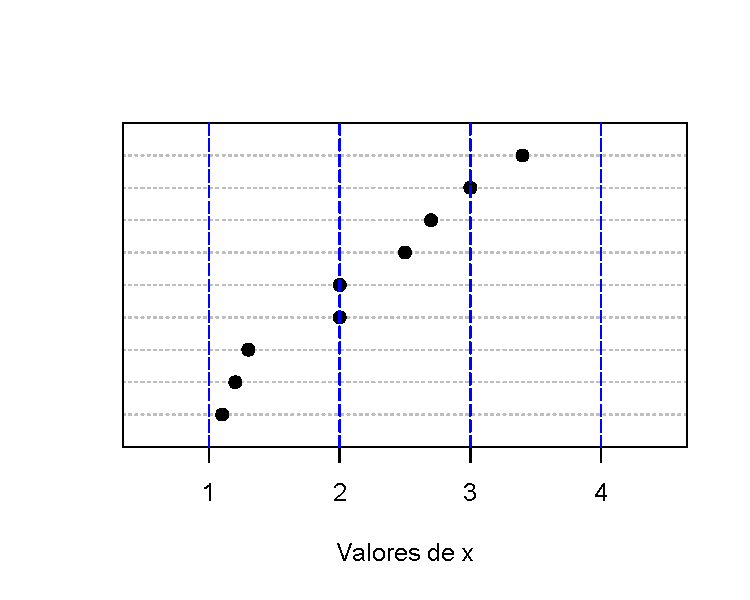
\includegraphics{Manual_de_R_files/figure-latex/dots-1.pdf}
\caption{\label{fig:dots}Ubicación de los puntos del ejemplo con límites en
color azul.}
\end{figure}

A continuación se presenta el código para obtener la tabla de frecuencia
usando \texttt{rigth=TRUE}, los resultados se almacenan en el objeto
\texttt{res3} y se solicitan sólo los dos primeros elementos que
corresponden a los límites y frecuencias.

\begin{Shaded}
\begin{Highlighting}[]
\NormalTok{res3 <-}\StringTok{ }\KeywordTok{hist}\NormalTok{(x, }\DataTypeTok{breaks=}\KeywordTok{c}\NormalTok{(}\DecValTok{1}\NormalTok{, }\DecValTok{2}\NormalTok{, }\DecValTok{3}\NormalTok{, }\DecValTok{4}\NormalTok{), }\DataTypeTok{right=}\OtherTok{TRUE}\NormalTok{, }\DataTypeTok{plot=}\OtherTok{FALSE}\NormalTok{)}
\NormalTok{res3[}\DecValTok{1}\NormalTok{:}\DecValTok{2}\NormalTok{]}
\end{Highlighting}
\end{Shaded}

\begin{verbatim}
## $breaks
## [1] 1 2 3 4
## 
## $counts
## [1] 5 3 1
\end{verbatim}

Ahora vamos a repetir la tabla pero usando \texttt{rigth=FALSE} para ver
la diferencia, en \texttt{res4} están los resultados.

\begin{Shaded}
\begin{Highlighting}[]
\NormalTok{res4 <-}\StringTok{ }\KeywordTok{hist}\NormalTok{(x, }\DataTypeTok{breaks=}\KeywordTok{c}\NormalTok{(}\DecValTok{1}\NormalTok{, }\DecValTok{2}\NormalTok{, }\DecValTok{3}\NormalTok{, }\DecValTok{4}\NormalTok{), }\DataTypeTok{right=}\OtherTok{FALSE}\NormalTok{, }\DataTypeTok{plot=}\OtherTok{FALSE}\NormalTok{)}
\NormalTok{res4[}\DecValTok{1}\NormalTok{:}\DecValTok{2}\NormalTok{]}
\end{Highlighting}
\end{Shaded}

\begin{verbatim}
## $breaks
## [1] 1 2 3 4
## 
## $counts
## [1] 3 4 2
\end{verbatim}

Al comparar los últimos dos resultados vemos que la primera frecuencia
es 5 cuando \texttt{right=TRUE} porque los intervalos se consideran
cerrados a la derecha.

Ahora vamos a construir una tabla de frecuencia usando \texttt{FALSE}
para los parámetros \texttt{include.lowest} y \texttt{right}.

\begin{Shaded}
\begin{Highlighting}[]
\NormalTok{res5 <-}\StringTok{ }\KeywordTok{hist}\NormalTok{(x, }\DataTypeTok{breaks=}\KeywordTok{c}\NormalTok{(}\DecValTok{1}\NormalTok{, }\DecValTok{2}\NormalTok{, }\DecValTok{3}\NormalTok{, }\DecValTok{4}\NormalTok{),}
             \DataTypeTok{include.lowest=}\OtherTok{FALSE}\NormalTok{, }\DataTypeTok{right=}\OtherTok{FALSE}\NormalTok{,}
             \DataTypeTok{plot=}\OtherTok{FALSE}\NormalTok{)}
\NormalTok{res5[}\DecValTok{1}\NormalTok{:}\DecValTok{2}\NormalTok{]}
\end{Highlighting}
\end{Shaded}

\begin{verbatim}
## $breaks
## [1] 1 2 3 4
## 
## $counts
## [1] 3 4 2
\end{verbatim}

De este último resultado se ve claramente el efecto de los parámetros
\texttt{include.lowest} y \texttt{right} en la construcción de tablas de
frecuencia.

\section*{EJERCICIOS}\label{ejercicios-4}


Use funciones o procedimientos (varias líneas) de \proglang{R} para
responder cada una de las siguientes preguntas.

En el Cuadro \ref{tab:toy} se presenta una base de datos sencilla. Lea
la base de datos usando la funcion \texttt{read.table} y construya lo
que se solicita a continuación.

\begin{enumerate}
\def\labelenumi{\arabic{enumi}.}
\tightlist
\item
  Construya una tabla de frecuencia absoluta para la variable
  pasatiempo.
\item
  Construya una tabla de frecuencia relativa para la variable fuma.
\item
  Construya una tabla de frecuencia relativa para las variables
  pasatiempo y fuma.
\item
  ¿Qué porcentaje de de los que no fuman tienen como pasatiempo la
  lectura.
\item
  ¿Qué porcentaje de los que corren no fuman?
\end{enumerate}

\chapter{\texorpdfstring{Medidas de tendencia central
\label{central}}{Medidas de tendencia central }}\label{medidas-de-tendencia-central}

En este capítulo se mostrará cómo obtener las diferentes medidas de
tendencia central con \proglang{R}.

Para ilustrar el uso de las funciones se utilizará una base de datos
llamada \textbf{medidas del cuerpo}, esta base de datos cuenta con 6
variables registradas a un grupo de 36 estudiantes de la universidad.
Las variables son:

\begin{enumerate}
\def\labelenumi{\arabic{enumi}.}
\tightlist
\item
  \texttt{edad} del estudiante (años),
\item
  \texttt{peso} del estudiante (kilogramos),
\item
  \texttt{altura} del estudiante (centímetros),
\item
  \texttt{sexo} del estudiante (Hombre, Mujer),
\item
  \texttt{muneca}: perímetro de la muñeca derecha (centímetros),
\item
  \texttt{biceps}: perímetro del biceps derecho (centímetros).
\end{enumerate}

A continuación se presenta el código para definir la url donde están los
datos, para cargar la base de datos en R y para mostrar por pantalla un
encabezado (usando \texttt{head}) de la base de datos.

\begin{Shaded}
\begin{Highlighting}[]
\NormalTok{url <-}\StringTok{ 'https://raw.githubusercontent.com/fhernanb/datos/master/medidas_cuerpo'}
\NormalTok{datos <-}\StringTok{ }\KeywordTok{read.table}\NormalTok{(}\DataTypeTok{file=}\NormalTok{url, }\DataTypeTok{header=}\NormalTok{T)}
\KeywordTok{head}\NormalTok{(datos)  }\CommentTok{# Para ver el encabezado de la base de datos}
\end{Highlighting}
\end{Shaded}

\begin{verbatim}
##   edad peso altura   sexo muneca biceps
## 1   43 87.3  188.0 Hombre   12.2   35.8
## 2   65 80.0  174.0 Hombre   12.0   35.0
## 3   45 82.3  176.5 Hombre   11.2   38.5
## 4   37 73.6  180.3 Hombre   11.2   32.2
## 5   55 74.1  167.6 Hombre   11.8   32.9
## 6   33 85.9  188.0 Hombre   12.4   38.5
\end{verbatim}

\section{\texorpdfstring{Media \index{media}
\index{mean}}{Media  }}\label{media}

Para calcular la media de una variable cuantitativa se usa la función
\texttt{mean}. Los argumentos básicos de la función \texttt{mean} son
dos y se muestran a continuación.

\begin{Shaded}
\begin{Highlighting}[]
\KeywordTok{mean}\NormalTok{(x, }\DataTypeTok{na.rm =} \OtherTok{FALSE}\NormalTok{)}
\end{Highlighting}
\end{Shaded}

En el parámetro \texttt{x} se indica la variable de interés para la cual
se quiere calcular la media, el parámetro \texttt{na.rm} es un valor
lógico que en caso de ser \texttt{TRUE}, significa que se deben remover
las observaciones con \texttt{NA}, el valor por defecto para este
parámetro es \texttt{FALSE}.

\subsection*{Ejemplo}\label{ejemplo-25}


Suponga que queremos obtener la altura media del grupo de estudiantes.

Para encontrar la media general se usa la función \texttt{mean} sobre el
vector númerico \texttt{datos\$altura}.

\begin{Shaded}
\begin{Highlighting}[]
\KeywordTok{mean}\NormalTok{(}\DataTypeTok{x=}\NormalTok{datos$altura)}
\end{Highlighting}
\end{Shaded}

\begin{verbatim}
## [1] 171.6
\end{verbatim}

Del anterior resultado podemos decir que la estatura media o promedio de
los estudiantes es 171.5556 centímetros.

\subsection*{Ejemplo}\label{ejemplo-26}


Suponga que ahora queremos la altura media pero diferenciando por sexo.

Para hacer esto se debe primero dividir o partir el vector de altura
según los niveles de la variable sexo, esto se consigue por medio de la
función \texttt{split} y el resultado será una lista con tantos
elementos como niveles tenga la variable sexo. Luego a cada uno de los
elementos de la lista se le aplica la función \texttt{mean} con la ayuda
de \texttt{sapply} o \texttt{tapply}. A continuación el código completo
para obtener las alturas medias para hombres y mujeres.

\begin{Shaded}
\begin{Highlighting}[]
\KeywordTok{sapply}\NormalTok{(}\KeywordTok{split}\NormalTok{(}\DataTypeTok{x=}\NormalTok{datos$altura, }\DataTypeTok{f=}\NormalTok{datos$sexo), mean)}
\end{Highlighting}
\end{Shaded}

\begin{verbatim}
## Hombre  Mujer 
##  179.1  164.0
\end{verbatim}

El resultado es un vector con dos elementos, vemos que la altura media
para hombres es 179.0778 centímetros y que para las mujeres es de
164.0333 centímetros.

¿Qué sucede si se usa \texttt{tapply} en lugar de \texttt{sapply}?
Substituya en el código anterior la función \texttt{sapply} por
\texttt{tapply} y observe la diferencia entre los resultados.

\subsection*{Ejemplo}\label{ejemplo-27}


Suponga que se tiene el vector \texttt{edad} con las edades de siete
personas y supóngase que para el individuo cinco no se tiene información
de su edad, eso significa que el vector tendrá un \texttt{NA} en la
quinta posición.

¿Cuál será la edad promedio del grupo de personas?

\begin{Shaded}
\begin{Highlighting}[]
\NormalTok{edad <-}\StringTok{ }\KeywordTok{c}\NormalTok{(}\DecValTok{18}\NormalTok{, }\DecValTok{23}\NormalTok{, }\DecValTok{26}\NormalTok{, }\DecValTok{32}\NormalTok{, }\OtherTok{NA}\NormalTok{, }\DecValTok{32}\NormalTok{, }\DecValTok{29}\NormalTok{)}
\KeywordTok{mean}\NormalTok{(}\DataTypeTok{x=}\NormalTok{edad)}
\end{Highlighting}
\end{Shaded}

\begin{verbatim}
## [1] NA
\end{verbatim}

Al correr el código anterior se obtiene un error y es debido al símbolo
\texttt{NA} en la quinta posición. Para calcular la media sólo con los
datos de los cuales se tiene información, se incluye el argumento
\texttt{na.rm\ =\ TRUE} para que R remueva los \texttt{NA}. El código
correcto a usar en este caso es:

\begin{Shaded}
\begin{Highlighting}[]
\KeywordTok{mean}\NormalTok{(}\DataTypeTok{x=}\NormalTok{edad, }\DataTypeTok{na.rm=}\OtherTok{TRUE}\NormalTok{)}
\end{Highlighting}
\end{Shaded}

\begin{verbatim}
## [1] 26.67
\end{verbatim}

De este último resultado se obtiene que la edad promedio de los
individuos es 26.67 años.

\section{\texorpdfstring{Mediana \index{mediana}
\index{median}}{Mediana  }}\label{mediana}

Para calcular la mediana de una variable cantitativa se usa la función
\texttt{median}. Los argumentos básicos de la función \texttt{median}
son dos y se muestran a continuación.

\begin{Shaded}
\begin{Highlighting}[]
\KeywordTok{median}\NormalTok{(x, }\DataTypeTok{na.rm =} \OtherTok{FALSE}\NormalTok{)}
\end{Highlighting}
\end{Shaded}

En el parámetro \texttt{x} se indica la variable de interés para la cual
se quiere calcular la mediana, el parámetro \texttt{na.rm} es un valor
lógico que en caso de ser \texttt{TRUE}, significa que se deben remover
las observaciones con \texttt{NA}, el valor por defecto para este
parámetro es \texttt{FALSE}.

\subsection*{Ejemplo}\label{ejemplo-28}


Calcular la edad mediana para los estudiantes de la base de datos.

Para obtener la mediana usamos el siguiente código:

\begin{Shaded}
\begin{Highlighting}[]
\KeywordTok{median}\NormalTok{(}\DataTypeTok{x=}\NormalTok{datos$edad)}
\end{Highlighting}
\end{Shaded}

\begin{verbatim}
## [1] 28
\end{verbatim}

y obtenemos que la mitad de los estudiantes tienen edades mayores o
iguales a 28 años.

El resultado anterior se pudo haber obtenido con la función
\texttt{quantile} e indicando que se desea el cuantil 50 así:

\begin{Shaded}
\begin{Highlighting}[]
\KeywordTok{quantile}\NormalTok{(}\DataTypeTok{x=}\NormalTok{datos$edad, }\DataTypeTok{probs=}\FloatTok{0.5}\NormalTok{)}
\end{Highlighting}
\end{Shaded}

\begin{verbatim}
## 50% 
##  28
\end{verbatim}

\section{\texorpdfstring{Moda \index{moda}}{Moda }}\label{moda}

La moda de una variable cuantitativa corresponde a valor o valores que
más se repiten, una forma sencilla de encontrar la moda es construir una
tabla de frecuencias y observar los valores con mayor frecuencia.

\subsection*{Ejemplo}\label{ejemplo-29}


Calcular la moda para la variable edad de la base de datos de
estudiantes.

Se construye la tabla con la función \texttt{table} y se crea el objeto
\texttt{tabla} para almacenarla.

\begin{Shaded}
\begin{Highlighting}[]
\NormalTok{tabla <-}\StringTok{ }\KeywordTok{table}\NormalTok{(datos$edad)}
\NormalTok{tabla}
\end{Highlighting}
\end{Shaded}

\begin{verbatim}
## 
## 19 20 21 22 23 24 25 26 28 29 30 32 33 35 37 40 43 45 
##  1  1  1  3  2  1  5  3  2  1  2  1  1  2  3  1  2  1 
## 51 55 65 
##  1  1  1
\end{verbatim}

Al mirar con detalle la tabla anterior se observa que el valor que más
se repite es la edad de 25 años en 5 ocasiones. Si la tabla hubiese sido
mayor, la inspección visual nos podría tomar unos segundos o hasta
minutos y podríamos equivocarnos, por esa razón es mejor ordenar los
resultados de la tabla.

Para observar los valores con mayor frecuencia de la tabla se puede
ordenar la tabla usando la función \texttt{sort} de la siguiente manera:

\begin{Shaded}
\begin{Highlighting}[]
\KeywordTok{sort}\NormalTok{(tabla, }\DataTypeTok{decreasing=}\OtherTok{TRUE}\NormalTok{)}
\end{Highlighting}
\end{Shaded}

\begin{verbatim}
## 
## 25 22 26 37 23 28 30 35 43 19 20 21 24 29 32 33 40 45 
##  5  3  3  3  2  2  2  2  2  1  1  1  1  1  1  1  1  1 
## 51 55 65 
##  1  1  1
\end{verbatim}

De esta manera se ve fácilmente que la variable edad es unimodal con
valor de 25 años.

\chapter{\texorpdfstring{Medidas de variabilidad
\label{varia}}{Medidas de variabilidad }}\label{medidas-de-variabilidad}

En este capítulo se mostrará cómo obtener las diferentes medidas de
variabilidad con \proglang{R}.

Para ilustrar el uso de las funciones se utilizará la base de datos
llamada \textbf{aptos2015}, esta base de datos cuenta con 11 variables
registradas a apartamentos usados en la ciudad de Medellín. Las
variables de la base de datos son:

\begin{enumerate}
\def\labelenumi{\arabic{enumi}.}
\tightlist
\item
  \texttt{precio}: precio de venta del apartamento (millones de pesos),
\item
  \texttt{mt2}: área del apartamento (\(m^2\)),
\item
  \texttt{ubicacion}: lugar de ubicación del aparamentos en la ciudad
  (cualitativa),
\item
  \texttt{estrato}: nivel socioeconómico donde está el apartamento (2 a
  6),
\item
  \texttt{alcobas}: número de alcobas del apartamento,
\item
  \texttt{banos}: número de baños del apartamento,
\item
  \texttt{balcon}: si el apartamento tiene balcón (si o no),
\item
  \texttt{parqueadero}: si el apartamento tiene parqueadero (si o no),
\item
  \texttt{administracion}: valor mensual del servicio de administración
  (millones de pesos),
\item
  \texttt{avaluo}: valor del apartamento en escrituras (millones de
  pesos),
\item
  \texttt{terminado}: si el apartamento se encuentra terminado (si o
  no).
\end{enumerate}

A continuación se presenta el código para definir la url donde están los
datos, para cargar la base de datos en R y para mostrar por pantalla un
encabezado (usando \texttt{head}) de la base de datos.

\begin{Shaded}
\begin{Highlighting}[]
\NormalTok{url <-}\StringTok{ 'https://raw.githubusercontent.com/fhernanb/datos/master/aptos2015'}
\NormalTok{datos <-}\StringTok{ }\KeywordTok{read.table}\NormalTok{(}\DataTypeTok{file=}\NormalTok{url, }\DataTypeTok{header=}\NormalTok{T)}
\KeywordTok{head}\NormalTok{(datos)  }\CommentTok{# Para ver el encabezado de la base de datos}
\end{Highlighting}
\end{Shaded}

\begin{verbatim}
##   precio   mt2 ubicacion estrato alcobas banos balcon
## 1     79 43.16     norte       3       3     1     si
## 2     93 56.92     norte       2       2     1     si
## 3    100 66.40     norte       3       2     2     no
## 4    123 61.85     norte       2       3     2     si
## 5    135 89.80     norte       4       3     2     si
## 6    140 71.00     norte       3       3     2     no
##   parqueadero administracion avaluo terminado
## 1          si          0.050  14.92        no
## 2          si          0.069  27.00        si
## 3          no          0.000  15.74        no
## 4          si          0.130  27.00        no
## 5          no          0.000  39.57        si
## 6          si          0.120  31.15        si
\end{verbatim}

\section{\texorpdfstring{Rango \index{rango}
\index{range}}{Rango  }}\label{rango}

Para calcular el rango de una variable cuantitativa se usa la función
\texttt{range}. Los argumentos básicos de la función \texttt{range} son
dos y se muestran abajo.

\begin{Shaded}
\begin{Highlighting}[]
\KeywordTok{range}\NormalTok{(x, }\DataTypeTok{na.rm =} \OtherTok{FALSE}\NormalTok{)}
\end{Highlighting}
\end{Shaded}

En el parámetro \texttt{x} se indica la variable de interés para la cual
se quiere calcular el rango, el parámetro \texttt{na.rm} es un valor
lógico que en caso de ser \texttt{TRUE}, significa que se deben remover
las observaciones con \texttt{NA}, el valor por defecto para este
parámetro es \texttt{FALSE}.

La función \texttt{range} entrega el valor mínimo y máximo de la
variable ingresada y el valor de rango se puede obtener restando del
valor máximo el valor mínimo.

\subsection*{Ejemplo}\label{ejemplo-30}


Suponga que queremos obtener el rango para la variable precio de los
apartamentos.

Para obtener el rango usamos el siguiente código.

\begin{Shaded}
\begin{Highlighting}[]
\KeywordTok{range}\NormalTok{(datos$precio)}
\end{Highlighting}
\end{Shaded}

\begin{verbatim}
## [1]   25 1700
\end{verbatim}

\begin{Shaded}
\begin{Highlighting}[]
\KeywordTok{max}\NormalTok{(datos$precio) -}\StringTok{ }\KeywordTok{min}\NormalTok{(datos$precio)}
\end{Highlighting}
\end{Shaded}

\begin{verbatim}
## [1] 1675
\end{verbatim}

Del resultado anterior podemos ver que los precios de todos los
apartamentos van desde 25 hasta 1700 millones de pesos, es decir, el
rango de la variable precio es 1675 millones de pesos.

\subsection*{Ejemplo}\label{ejemplo-31}


Suponga que queremos obtener nuevamente el rango para la variable precio
de los apartamentos pero diferenciando por el estrato.

Primero vamos a crear una función auxiliar llamada \texttt{myrange} que
calculará el rango directamente (\(max - min\)). Luego vamos a partir la
información de los precios por cada estrato usando \texttt{split}, la
partición se almacenará en la lista \texttt{precios}. Finalmente se
aplicará la función \texttt{myrange} a la lista \texttt{precios} para
obtener los rangos del precio por estrato socioeconómico. El código para
realizar esto se muestra a continuación.

\begin{Shaded}
\begin{Highlighting}[]
\NormalTok{myrange <-}\StringTok{ }\NormalTok{function(x) }\KeywordTok{max}\NormalTok{(x) -}\StringTok{ }\KeywordTok{min}\NormalTok{(x)}
\NormalTok{precios <-}\StringTok{ }\KeywordTok{split}\NormalTok{(datos$precio, }\DataTypeTok{f=}\NormalTok{datos$estrato)}
\KeywordTok{sapply}\NormalTok{(precios, myrange)}
\end{Highlighting}
\end{Shaded}

\begin{verbatim}
##    2    3    4    5    6 
##  103  225  610 1325 1560
\end{verbatim}

De los resultados podemos ver claramente que a medida que aumenta de
estrato el rango (variabilidad) del precio de los apartamentos aumenta.
Apartamentos de estrato bajo tienden a tener precios similares mientras
que los precios de venta para apartamentos de estratos altos tienden a
ser muy diferentes entre si.

\section{\texorpdfstring{Desviación estándar muestral (\(S\))
\index{desviación}
\index{sd}}{Desviación estándar muestral (S)  }}\label{desviacion-estandar-muestral-s}

Para calcular la desviación muestral de una variable cuantitativa se usa
la función \texttt{sd}. Los argumentos básicos de la función \texttt{sd}
son dos y se muestran abajo.

\begin{Shaded}
\begin{Highlighting}[]
\KeywordTok{sd}\NormalTok{(x, }\DataTypeTok{na.rm =} \OtherTok{FALSE}\NormalTok{)}
\end{Highlighting}
\end{Shaded}

En el parámetro \texttt{x} se indica la variable de interés para la cual
se quiere calcular la desviación estándar muestral, el parámetro
\texttt{na.rm} es un valor lógico que en caso de ser \texttt{TRUE},
significa que se deben remover las observaciones con \texttt{NA}, el
valor por defecto para este parámetro es \texttt{FALSE}.

\subsection*{Ejemplo}\label{ejemplo-32}


Suponga que queremos obtener la desviación estándar muestral para la
variable precio de los apartamentos.

Para obtener la desviación solicitada usamos el siguiente código:

\begin{Shaded}
\begin{Highlighting}[]
\KeywordTok{sd}\NormalTok{(}\DataTypeTok{x=}\NormalTok{datos$precio)}
\end{Highlighting}
\end{Shaded}

\begin{verbatim}
## [1] 247.6
\end{verbatim}

\subsection*{Ejemplo}\label{ejemplo-33}


Calcular la desviación estándar \textbf{poblacional} (\(\sigma\)) para
el siguiente conjunto de 5 observaciones: 12, 25, 32, 15, 26.

Recordemos que las expresiones matemáticas para obtener \(S\) y
\(\sigma\) son muy similares, la diferencia está en el denominador, para
\(S\) el denominador es \(n-1\) mientras que para \(\sigma\) es \(n\).
Teniendo esto en cuenta podemos calcular la desviación poblacional
apoyándonos en la función \texttt{sd}, para esto podemos construir una
función llamada \texttt{Sigma} que calcule la desviación poblacional, a
continuación el código necesario.

\begin{Shaded}
\begin{Highlighting}[]
\NormalTok{Sigma <-}\StringTok{ }\NormalTok{function(x) \{}
  \NormalTok{n <-}\StringTok{ }\KeywordTok{length}\NormalTok{(x)}
  \KeywordTok{sd}\NormalTok{(x) *}\StringTok{ }\NormalTok{(n}\DecValTok{-1}\NormalTok{) /}\StringTok{ }\NormalTok{n}
\NormalTok{\} }
\end{Highlighting}
\end{Shaded}

Ahora para obtener la desviación estándar \textbf{poblacional} de los
datos usamos el siguiente código.

\begin{Shaded}
\begin{Highlighting}[]
\NormalTok{y <-}\StringTok{ }\KeywordTok{c}\NormalTok{(}\DecValTok{12}\NormalTok{, }\DecValTok{25}\NormalTok{, }\DecValTok{32}\NormalTok{, }\DecValTok{15}\NormalTok{, }\DecValTok{26}\NormalTok{)}
\KeywordTok{Sigma}\NormalTok{(y)}
\end{Highlighting}
\end{Shaded}

\begin{verbatim}
## [1] 6.621
\end{verbatim}

\section{\texorpdfstring{Varianza muestral (\(S^2\)) \index{varianza}
\index{var}}{Varianza muestral (S\^{}2)  }}\label{varianza-muestral-s2}

Para calcular la varianza muestral de una variable cuantitativa se usa
la función \texttt{var}. Los argumentos básicos de la función
\texttt{var} son dos y se muestran abajo.

\begin{Shaded}
\begin{Highlighting}[]
\KeywordTok{var}\NormalTok{(x, }\DataTypeTok{na.rm =} \OtherTok{FALSE}\NormalTok{)}
\end{Highlighting}
\end{Shaded}

En el parámetro \texttt{x} se indica la variable de interés para la cual
se quiere calcular la varianza muestral, el parámetro \texttt{na.rm} es
un valor lógico que en caso de ser \texttt{TRUE}, significa que se deben
remover las observaciones con \texttt{NA}, el valor por defecto para
este parámetro es \texttt{FALSE}.

\subsection*{Ejemplo}\label{ejemplo-34}


Suponga que queremos determinar cuál región en la ciudad presenta mayor
varianza en los precios de los apartamentos.

Para realizar esto debemos usar en conjunto la función \texttt{split},
\texttt{sapply} y \texttt{var} ya que se quiere la varianza de una
variable (\texttt{precio}) dado los valores de otra variable
(\texttt{ubicacion}). El código para obtener las varianzas es el
siguiente.

\begin{Shaded}
\begin{Highlighting}[]
\NormalTok{precios <-}\StringTok{ }\KeywordTok{split}\NormalTok{(datos$precio, }\DataTypeTok{f=}\NormalTok{datos$ubicacion)}
\KeywordTok{sapply}\NormalTok{(precios, var)}
\end{Highlighting}
\end{Shaded}

\begin{verbatim}
##     aburra sur belen guayabal         centro 
##           4169           2528           2588 
##       laureles          norte      occidente 
##          25351           1009           3596 
##        poblado 
##          84497
\end{verbatim}

De los resultados anteriores se nota que los apartamentos ubicados en el
Poblado tienen la mayor variabilidad en el precio, este resultado se
confirma al dibujar un boxplot para la variable precio dada la
ubicación, en la Figura \ref{fig:box1} se muestra el boxplot y se ve
claramente la dispersión de los precios en el Poblado. El código usado
para generar la Figura \ref{fig:box1} se presenta a continuación.

\begin{Shaded}
\begin{Highlighting}[]
\KeywordTok{with}\NormalTok{(datos, }\KeywordTok{boxplot}\NormalTok{(precio ~}\StringTok{ }\NormalTok{ubicacion, }\DataTypeTok{ylab=}\StringTok{'Precio (millones)'}\NormalTok{))}
\end{Highlighting}
\end{Shaded}

\begin{figure}[htbp]
\centering
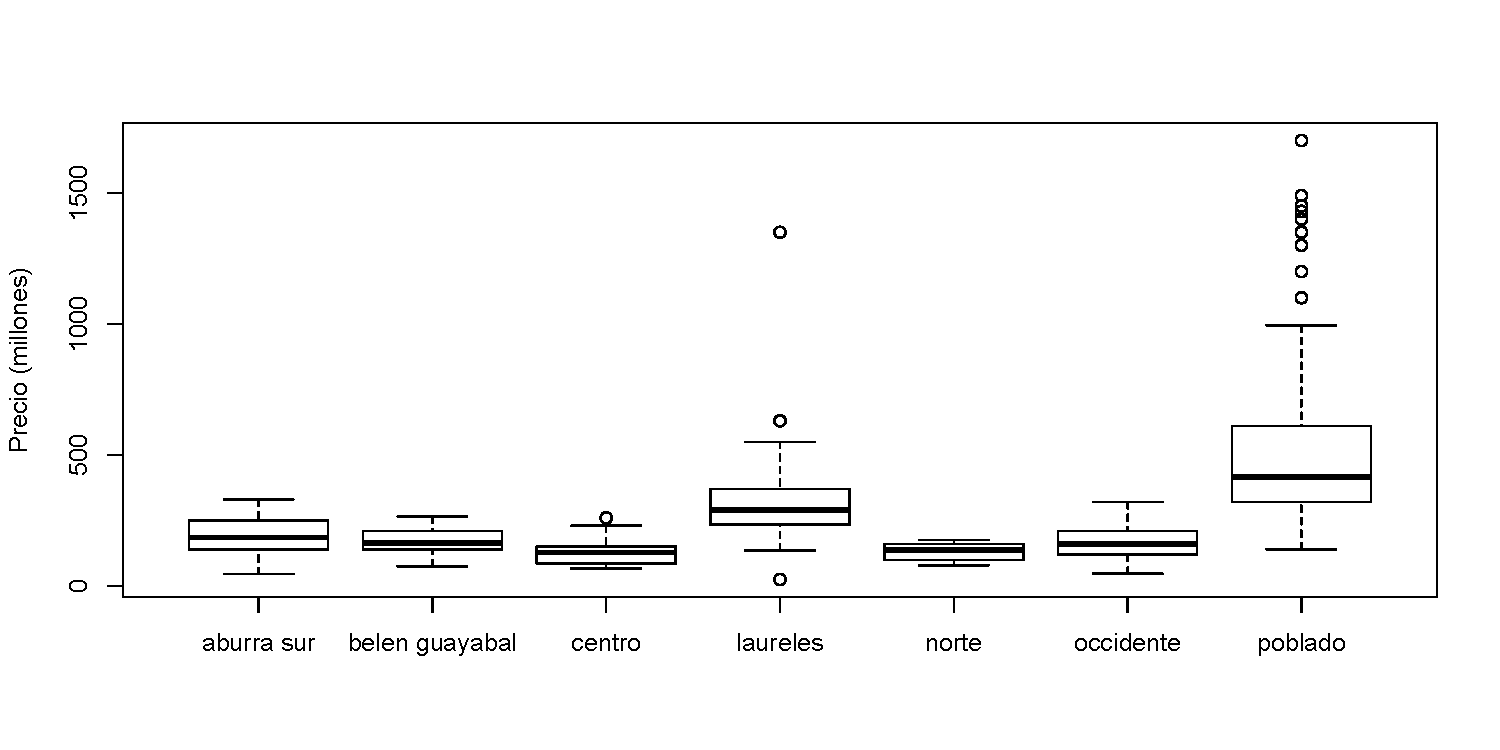
\includegraphics{Manual_de_R_files/figure-latex/box1-1.pdf}
\caption{\label{fig:box1}Boxplot para el precio de los apartamentos dada la
ubicación.}
\end{figure}

\subsection*{Ejemplo}\label{ejemplo-35}


¿Son los resultados de la función \texttt{var} los mismos que los
resultados de la función \texttt{sd} elevados al cuadrado?

La respuesta es \textbf{NO}. La función \texttt{sd} se aplica sólo a
vectores mientras que la función \texttt{var} de puede aplicar tanto a
vectores como a marcos de datos. Al ser aplicada a marcos de datos
numéricos se obtiene una matriz en que la diagonal representa las
varianzas de las de cada una de las variables mientras que arriba y
abajo de la diagonal se encuentran las covarianzas entre pares de
variables.

Por ejemplo, si aplicamos la función \texttt{var} al marco de datos sólo
con las variables precio, área y avaluo se obtiene una matriz de
dimensión \(3 \times 3\), a continuación el código usado.

\begin{Shaded}
\begin{Highlighting}[]
\KeywordTok{var}\NormalTok{(datos[, }\KeywordTok{c}\NormalTok{(}\StringTok{'precio'}\NormalTok{, }\StringTok{'mt2'}\NormalTok{, }\StringTok{'avaluo'}\NormalTok{)])}
\end{Highlighting}
\end{Shaded}

\begin{verbatim}
##        precio   mt2 avaluo
## precio  61313 15874  33056
## mt2     15874  5579   9508
## avaluo  33056  9508  28589
\end{verbatim}

Del anterior resultado se observa la matriz de varianzas y covarianzas
de dimensión \(3 \times 3\).

\section{\texorpdfstring{Coeficiente de variación (\(CV\))
\index{coeficiente de variación}}{Coeficiente de variación (CV) }}\label{coeficiente-de-variacion-cv}

El coeficiente de variación se define como \(CV=s/\bar{x}\) y es muy
sencillo de obtenerlo, la función \texttt{CV} mostrada abajo permite
calcularlo.

\begin{Shaded}
\begin{Highlighting}[]
\NormalTok{CV <-}\StringTok{ }\NormalTok{function(x, }\DataTypeTok{na.rm =} \OtherTok{FALSE}\NormalTok{) \{}
  \KeywordTok{sd}\NormalTok{(x, }\DataTypeTok{na.rm=}\NormalTok{na.rm) /}\StringTok{ }\KeywordTok{mean}\NormalTok{(x, }\DataTypeTok{na.rm=}\NormalTok{na.rm)}
\NormalTok{\}}
\end{Highlighting}
\end{Shaded}

\subsection*{Ejemplo}\label{ejemplo-36}


Calcular el \(CV\) para el vector \texttt{w} definido a continuación.

\begin{Shaded}
\begin{Highlighting}[]
\NormalTok{w <-}\StringTok{ }\KeywordTok{c}\NormalTok{(}\DecValTok{5}\NormalTok{, -}\DecValTok{3}\NormalTok{, }\OtherTok{NA}\NormalTok{, }\DecValTok{8}\NormalTok{, }\DecValTok{8}\NormalTok{, }\DecValTok{7}\NormalTok{)}
\end{Highlighting}
\end{Shaded}

Vemos que el vector \texttt{w} tiene 6 observaciones y la tercera de
ellas es un \texttt{NA}. Lo correcto aquí es usar la función \texttt{CV}
definida antes pero indicándole que remueva los valores faltantes, para
eso se usa el siguiente código.

\begin{Shaded}
\begin{Highlighting}[]
\KeywordTok{CV}\NormalTok{(}\DataTypeTok{x=}\NormalTok{w, }\DataTypeTok{na.rm=}\NormalTok{T)}
\end{Highlighting}
\end{Shaded}

\begin{verbatim}
## [1] 0.9274
\end{verbatim}

\chapter{\texorpdfstring{Medidas de posición
\label{posi}}{Medidas de posición }}\label{medidas-de-posicion}

En este capítulo se mostrará cómo obtener las diferentes medidas de
posición con \proglang{R}.

Para ilustrar el uso de las funciones se utilizará una base de datos
llamada \textbf{medidas del cuerpo}, esta base de datos cuenta con 6
variables registradas a un grupo de 36 estudiantes de la universidad.
Las variables son:

\begin{enumerate}
\def\labelenumi{\arabic{enumi}.}
\tightlist
\item
  \texttt{edad} del estudiante (años),
\item
  \texttt{peso} del estudiante (kilogramos),
\item
  \texttt{altura} del estudiante (centímetros),
\item
  \texttt{sexo} del estudiante (Hombre, Mujer),
\item
  \texttt{muneca}: perímetro de la muñeca derecha (centímetros),
\item
  \texttt{biceps}: perímetro del biceps derecho (centímetros).
\end{enumerate}

A continuación se presenta el código para definir la url donde están los
datos, para cargar la base de datos en R y para mostrar por pantalla un
encabezado (usando \texttt{head}) de la base de datos.

\begin{Shaded}
\begin{Highlighting}[]
\NormalTok{url <-}\StringTok{ 'https://raw.githubusercontent.com/fhernanb/datos/master/medidas_cuerpo'}
\NormalTok{datos <-}\StringTok{ }\KeywordTok{read.table}\NormalTok{(}\DataTypeTok{file=}\NormalTok{url, }\DataTypeTok{header=}\NormalTok{T)}
\KeywordTok{head}\NormalTok{(datos)  }\CommentTok{# Para ver el encabezado de la base de datos}
\end{Highlighting}
\end{Shaded}

\begin{verbatim}
##   edad peso altura   sexo muneca biceps
## 1   43 87.3  188.0 Hombre   12.2   35.8
## 2   65 80.0  174.0 Hombre   12.0   35.0
## 3   45 82.3  176.5 Hombre   11.2   38.5
## 4   37 73.6  180.3 Hombre   11.2   32.2
## 5   55 74.1  167.6 Hombre   11.8   32.9
## 6   33 85.9  188.0 Hombre   12.4   38.5
\end{verbatim}

\section{\texorpdfstring{Cuantiles \index{cuantiles} \index{quantile}
\index{cuartiles} \index{deciles}
\index{percentiles}}{Cuantiles     }}\label{cuantiles}

Para obtener cualquier cuantil (cuartiles, deciles y percentiles) se usa
la función \texttt{quantile}. Los argumentos básicos de la función
\texttt{quantile} son tres y se muestran a continuación.

\begin{Shaded}
\begin{Highlighting}[]
\KeywordTok{quantile}\NormalTok{(x, probs, }\DataTypeTok{na.rm =} \OtherTok{FALSE}\NormalTok{)}
\end{Highlighting}
\end{Shaded}

En el parámetro \texttt{x} se indica la variable de interés para la cual
se quieren calcular los cuantiles, el parámetro \texttt{probs} sirve
para definir los cuantiles de interés y el parámetro \texttt{na.rm} es
un valor lógico que en caso de ser \texttt{TRUE}, significa que se deben
remover las observaciones con \texttt{NA}, el valor por defecto para
este parámetro es \texttt{FALSE}.

\subsection*{Ejemplo}\label{ejemplo-37}


Suponga que queremos obtener el percentil 5, la mediana y el decil 8 pa
la altura del grupo de estudiantes.

Se solicita el percentil 5, la mediana que es el percentil 50 y el decil
8 que corresponde al percentil 80, por lo tanto es necesario indicarle a
la función \texttt{quantile} que calcule los cuantiles para las
ubicaciones 0.05, 0.5 y 0.8, el código para obtener las tres medidas
solicitadas es el siguiente.

\begin{Shaded}
\begin{Highlighting}[]
\KeywordTok{quantile}\NormalTok{(}\DataTypeTok{x=}\NormalTok{datos$altura, }\DataTypeTok{probs=}\KeywordTok{c}\NormalTok{(}\FloatTok{0.05}\NormalTok{, }\FloatTok{0.5}\NormalTok{, }\FloatTok{0.8}\NormalTok{))}
\end{Highlighting}
\end{Shaded}

\begin{verbatim}
##    5%   50%   80% 
## 155.2 172.7 180.3
\end{verbatim}

\chapter{\texorpdfstring{Medidas de correlación
\label{correl}}{Medidas de correlación }}\label{medidas-de-correlacion}

En este capítulo se mostrará cómo obtener el coeficiente de correlación
lineal para variables cuantitativas.

\section{\texorpdfstring{Función \texttt{cor} \index{cor}
\index{correlación}}{Función cor  }}\label{funcion-cor}

La función \texttt{cor} permite calcular el coeficiente de correlación
de Pearson, Kendall o Spearman para dos variables cuantitativas. La
estructura de la función es la siguiente.

\begin{Shaded}
\begin{Highlighting}[]
\KeywordTok{cor}\NormalTok{(x, y, }\DataTypeTok{use=}\StringTok{"everything"}\NormalTok{,}
    \DataTypeTok{method=}\KeywordTok{c}\NormalTok{(}\StringTok{"pearson"}\NormalTok{, }\StringTok{"kendall"}\NormalTok{, }\StringTok{"spearman"}\NormalTok{))}
\end{Highlighting}
\end{Shaded}

Los parámetos de la función son:

\begin{itemize}
\tightlist
\item
  \texttt{x,\ y}: vectores cuantitativos.
\item
  \texttt{use}: parámetro que indica lo que se debe hacer cuando se
  presenten registros \texttt{NA} en alguno de los vectores. Las
  diferentes posibilidades son: \texttt{everything}, \texttt{all.obs},
  \texttt{complete.obs}, \texttt{na.or.complete} y
  \texttt{pairwise.complete.obs}, el valor por defecto es
  \texttt{everything}.
\item
  \texttt{method}: tipo de coeficiente de correlación a calcular, por
  defecto es \texttt{pearson}, otros valores posibles son
  \texttt{kendall} y \texttt{spearman}.
\end{itemize}

\subsection*{Ejemplo}\label{ejemplo-38}


Calcular el coeficiente de correlación de Pearson para las variables
área y precio de la base de datos sobre apartamentos usados.

Lo primero que se debe hacer es cargar la base de datos usando la url
apropiada. Luego de esto se usa la función \texttt{cor} sobre las
variables de interés. A continuación se muestra el código necesario.

\begin{Shaded}
\begin{Highlighting}[]
\NormalTok{url <-}\StringTok{ 'https://raw.githubusercontent.com/fhernanb/datos/master/aptos2015'}
\NormalTok{datos <-}\StringTok{ }\KeywordTok{read.table}\NormalTok{(}\DataTypeTok{file=}\NormalTok{url, }\DataTypeTok{header=}\NormalTok{T)}
\KeywordTok{cor}\NormalTok{(}\DataTypeTok{x=}\NormalTok{datos$mt2, }\DataTypeTok{y=}\NormalTok{datos$precio)}
\end{Highlighting}
\end{Shaded}

\begin{verbatim}
## [1] 0.8583
\end{verbatim}

Del resultado anterior vemos que existe una correlación de 0.8583 entre
las dos variables, eso significa que apartamentos de mayor área tienden
a tener precios de venta más alto. Este resultado se ilustra en la
Figura \ref{fig:disp}, se nota claramente que la nube de puntos tiene un
pendiente positiva y por eso el signo del coeficiente de correlación.

A continuación el código para generar la Figura \ref{fig:disp}.

\begin{Shaded}
\begin{Highlighting}[]
\KeywordTok{with}\NormalTok{(datos, }\KeywordTok{plot}\NormalTok{(}\DataTypeTok{x=}\NormalTok{mt2, }\DataTypeTok{y=}\NormalTok{precio, }\DataTypeTok{pch=}\DecValTok{20}\NormalTok{, }\DataTypeTok{col=}\StringTok{'blue'}\NormalTok{,}
                 \DataTypeTok{xlab=}\StringTok{'Área del apartamento'}\NormalTok{, }\DataTypeTok{las=}\DecValTok{1}\NormalTok{,}
                 \DataTypeTok{ylab=}\StringTok{'Precio del apartamento (millones COP)'}\NormalTok{))}
\end{Highlighting}
\end{Shaded}

\begin{figure}[htbp]
\centering
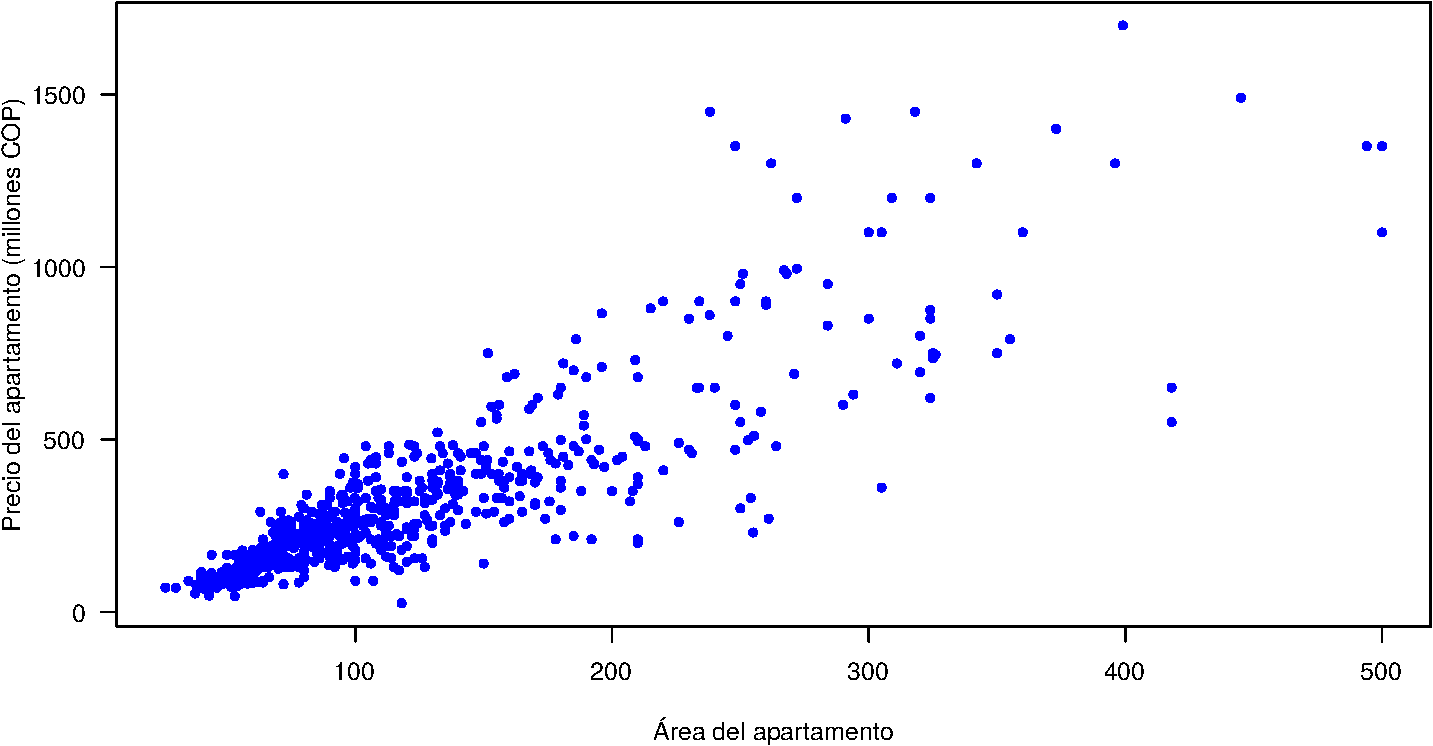
\includegraphics{Manual_de_R_files/figure-latex/disp-1.pdf}
\caption{\label{fig:disp}Diagrama de dispersión para precio versus área de
los apartamentos usados.}
\end{figure}

\subsection*{Ejemplo}\label{ejemplo-39}


Para las mismas variables del ejemplo anterior calcular los coeficientes
de correlación Kendall y Spearman.

A continuación el código para obtener lo solicitado.

\begin{Shaded}
\begin{Highlighting}[]
\KeywordTok{cor}\NormalTok{(}\DataTypeTok{x=}\NormalTok{datos$mt2, }\DataTypeTok{y=}\NormalTok{datos$precio, }\DataTypeTok{method=}\StringTok{'pearson'}\NormalTok{)}
\end{Highlighting}
\end{Shaded}

\begin{verbatim}
## [1] 0.8583
\end{verbatim}

\begin{Shaded}
\begin{Highlighting}[]
\KeywordTok{cor}\NormalTok{(}\DataTypeTok{x=}\NormalTok{datos$mt2, }\DataTypeTok{y=}\NormalTok{datos$precio, }\DataTypeTok{method=}\StringTok{'kendall'}\NormalTok{)}
\end{Highlighting}
\end{Shaded}

\begin{verbatim}
## [1] 0.6911
\end{verbatim}

\begin{Shaded}
\begin{Highlighting}[]
\KeywordTok{cor}\NormalTok{(}\DataTypeTok{x=}\NormalTok{datos$mt2, }\DataTypeTok{y=}\NormalTok{datos$precio, }\DataTypeTok{method=}\StringTok{'spearman'}\NormalTok{)}
\end{Highlighting}
\end{Shaded}

\begin{verbatim}
## [1] 0.8603
\end{verbatim}

\subsection*{Ejemplo}\label{ejemplo-40}


Para la base de datos de apartamentos usados, ¿cuáles de las variables
cuantitativas tienen mayor correlación?

Lo primero que debemos hacer es determinar cuáles son las cuantitativas
de la base de datos. Para obtener información de las variables que están
almacenadas en el marco de datos llamado \texttt{datos} usamos la
función \texttt{str} que muestra la estructura interna de objeto.

\begin{Shaded}
\begin{Highlighting}[]
\KeywordTok{str}\NormalTok{(datos)}
\end{Highlighting}
\end{Shaded}

\begin{verbatim}
## 'data.frame':    694 obs. of  11 variables:
##  $ precio        : num  79 93 100 123 135 140 145 160 160 175 ...
##  $ mt2           : num  43.2 56.9 66.4 61.9 89.8 ...
##  $ ubicacion     : Factor w/ 7 levels "aburra sur","belen guayabal",..: 5 5 5 5 5 5 5 5 5 5 ...
##  $ estrato       : int  3 2 3 2 4 3 3 3 4 4 ...
##  $ alcobas       : int  3 2 2 3 3 3 2 3 4 3 ...
##  $ banos         : int  1 1 2 2 2 2 2 2 2 2 ...
##  $ balcon        : Factor w/ 2 levels "no","si": 2 2 1 2 2 1 2 2 2 2 ...
##  $ parqueadero   : Factor w/ 2 levels "no","si": 2 2 1 2 1 2 2 2 1 2 ...
##  $ administracion: num  0.05 0.069 0 0.13 0 0.12 0.14 0.127 0 0.123 ...
##  $ avaluo        : num  14.9 27 15.7 27 39.6 ...
##  $ terminado     : Factor w/ 2 levels "no","si": 1 2 1 1 2 2 2 2 2 2 ...
\end{verbatim}

Del anterior resultado vemos que las variables precio, mt2, alcobas,
banos, administracion y avaluo son las variables cuantitativas, las
restantes son cualitativas (nominal u ordinal). Las posiciones de las
variables cuantitativas en el objeto \texttt{datos} son 1, 2, 5, 6, 9,
10, así podemos construir un marco de datos sólo con la información
cuantitativa, a continuación el código usado.

\begin{Shaded}
\begin{Highlighting}[]
\NormalTok{datos.cuanti <-}\StringTok{ }\NormalTok{datos[, }\KeywordTok{c}\NormalTok{(}\DecValTok{1}\NormalTok{, }\DecValTok{2}\NormalTok{, }\DecValTok{5}\NormalTok{, }\DecValTok{6}\NormalTok{, }\DecValTok{9}\NormalTok{, }\DecValTok{10}\NormalTok{)]}
\CommentTok{# La siguiente instrucción para editar los nombres de la variables}
\KeywordTok{colnames}\NormalTok{(datos.cuanti) <-}\StringTok{ }\KeywordTok{c}\NormalTok{(}\StringTok{'Precio'}\NormalTok{, }\StringTok{'Área'}\NormalTok{, }\StringTok{'Alcobas'}\NormalTok{,}
                            \StringTok{'Baños'}\NormalTok{, }\StringTok{'Admon'}\NormalTok{, }\StringTok{'Avaluo'}\NormalTok{)}
\NormalTok{M <-}\StringTok{ }\KeywordTok{round}\NormalTok{(}\KeywordTok{cor}\NormalTok{(datos.cuanti), }\DataTypeTok{digits=}\DecValTok{2}\NormalTok{)}
\NormalTok{M}
\end{Highlighting}
\end{Shaded}

\begin{verbatim}
##         Precio Área Alcobas Baños Admon Avaluo
## Precio    1.00 0.86    0.19  0.63  0.75   0.79
## Área      0.86 1.00    0.31  0.67  0.77   0.75
## Alcobas   0.19 0.31    1.00  0.35  0.16   0.15
## Baños     0.63 0.67    0.35  1.00  0.55   0.53
## Admon     0.75 0.77    0.16  0.55  1.00   0.70
## Avaluo    0.79 0.75    0.15  0.53  0.70   1.00
\end{verbatim}

El anterior resultado representa la matriz de correlaciones entre las
variables cuantitativas, se observa que la mayor correlación es entre
las variables precio y área del apartamento.

Es posible representar gráficamente la matriz de correlaciones
\texttt{M} por medio de la función \texttt{corrplot} del paquete
\textbf{corrplot}\index{corrplot} \citep{R-corrplot}, a continuación el
código para obtener su representación gráfica.

\begin{Shaded}
\begin{Highlighting}[]
\KeywordTok{library}\NormalTok{(}\StringTok{'corrplot'}\NormalTok{)  }\CommentTok{# Para cargar el paquete corrplot}
\KeywordTok{corrplot.mixed}\NormalTok{(M)}
\end{Highlighting}
\end{Shaded}

\begin{figure}[htbp]
\centering
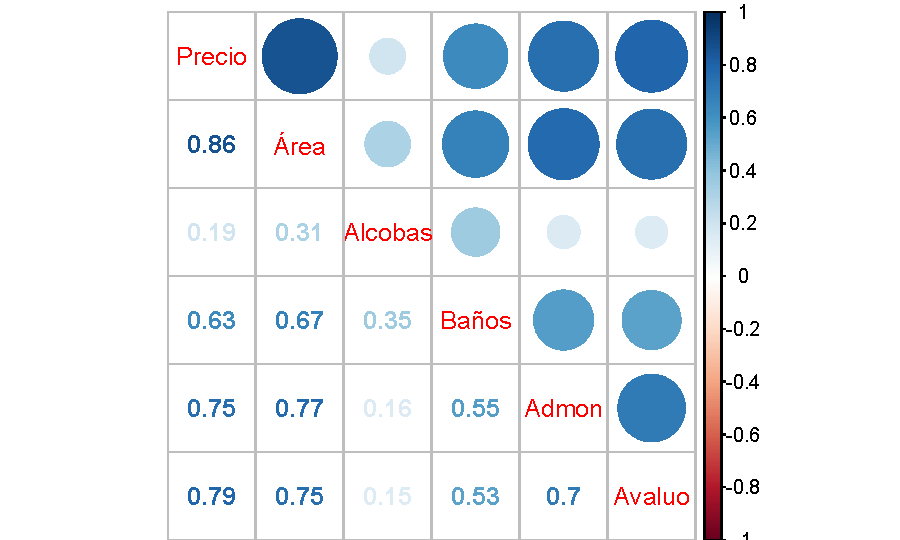
\includegraphics{Manual_de_R_files/figure-latex/corplot-1.pdf}
\caption{\label{fig:corplot}Matriz de coeficientes de correlación.}
\end{figure}

En la Figura \ref{fig:corplot} se muestra la matriz con los coeficientes
de correlación. En la diagonal de la Figura \ref{fig:corplot} están las
variables, por encima están unos círculos de colores, entre más
intensidad del color, ya sea azul o rojo, mayor es la correlación,
colores ténues significan correlación baja; el tamaño de los círculos
está asociado al valor absoluto de correlación. Por debajo de la
diagonal se observan los valores exactos de correlación en colores.

\BeginKnitrBlock{rmdtip}
La función \texttt{corrplot} es muy versátil, se pueden obtener
diferentes representaciones gráficas de la matriz de correlaciones, para
conocer las diferentes posibilidades recomendamos consultar este enlace:
\url{https://cran.r-project.org/web/packages/corrplot/vignettes/corrplot-intro.html}.
\EndKnitrBlock{rmdtip}

\subsection*{Ejemplo}\label{ejemplo-41}


Construya dos vectores hipotéticos con el gasto y ahorro de un grupo de
7 familias, incluya dos \texttt{NA}. Calcule el coeficiente de
correlación entre \texttt{ahorro} y \texttt{gasto}, use el parámetro
\texttt{use} para manejar los \texttt{NA}.

A continuación se presenta el código para crear los objetos
\texttt{ahorro} y \texttt{gasto} con datos ficticios. Observe que en el
primer caso donde se calcula la correlación no es posible obtener un
resultado debido a que por defecto
\texttt{use=\textquotesingle{}everything\textquotesingle{}} y por lo
tanto usa todas las observaciones incluyendo los \texttt{NA}. En el
segundo caso si se obtiene un valor para la correlación debido a que se
usó \texttt{use=\textquotesingle{}complete.obs\textquotesingle{}}.

\begin{Shaded}
\begin{Highlighting}[]
\NormalTok{gasto <-}\StringTok{ }\KeywordTok{c}\NormalTok{(}\DecValTok{170}\NormalTok{, }\DecValTok{230}\NormalTok{, }\DecValTok{120}\NormalTok{, }\DecValTok{156}\NormalTok{, }\DecValTok{256}\NormalTok{, }\OtherTok{NA}\NormalTok{, }\DecValTok{352}\NormalTok{)}
\NormalTok{ahorro <-}\StringTok{ }\KeywordTok{c}\NormalTok{(}\DecValTok{45}\NormalTok{, }\DecValTok{30}\NormalTok{, }\OtherTok{NA}\NormalTok{, }\DecValTok{35}\NormalTok{, }\DecValTok{15}\NormalTok{, }\DecValTok{65}\NormalTok{, }\DecValTok{15}\NormalTok{)}

\KeywordTok{cor}\NormalTok{(gasto, ahorro)}
\end{Highlighting}
\end{Shaded}

\begin{verbatim}
## [1] NA
\end{verbatim}

\begin{Shaded}
\begin{Highlighting}[]
\KeywordTok{cor}\NormalTok{(gasto, ahorro, }\DataTypeTok{use=}\StringTok{'complete.obs'}\NormalTok{)}
\end{Highlighting}
\end{Shaded}

\begin{verbatim}
## [1] -0.8465
\end{verbatim}

\section*{EJERCICIOS}\label{ejercicios-5}


Use funciones o procedimientos (varias líneas) de \proglang{R} para
responder cada una de las siguientes preguntas.

\begin{enumerate}
\def\labelenumi{\arabic{enumi}.}
\item
  Para cada uno de los estratos socioeconómicos, calcular el coeficiente
  de correlación lineal de Pearson para las variables precio y área de
  la base de datos de los apartamentos usados.
\item
  Calcular los coeficientes de correlación Pearson, Kendall y Spearman
  para las variables cuantitativas de la base de datos sobre medidas del
  cuerpo explicada en el Capítulo \ref{central}. La url con la
  información es la siguiente:
  \url{https://raw.githubusercontent.com/fhernanb/datos/master/medidas_cuerpo}
\item
  Represente gráficamente las matrices de correlación obtenidas en el
  ejercicio anterior.
\end{enumerate}

\chapter{Distribuciones discretas}\label{distribuciones-discretas}

En este capítulo se mostrarán las funciones de \proglang{R} para
distribuciones discretas.

\section{\texorpdfstring{Funciones disponibles para distribuciones
discretas
\index{distribuciones discretas}}{Funciones disponibles para distribuciones discretas }}\label{funciones-disponibles-para-distribuciones-discretas}

Para cada distribución discreta se tienen 4 funciones, a continuación el
listado de funciones y su utilidad.

\begin{Shaded}
\begin{Highlighting}[]
\KeywordTok{dxxx}\NormalTok{(x, ...)  }\CommentTok{# Función de masa de probabilidad, f(x)}
\KeywordTok{pxxx}\NormalTok{(q, ...)  }\CommentTok{# Función de distribución acumulada hasta q, F(x)}
\KeywordTok{qxxx}\NormalTok{(p, ...)  }\CommentTok{# Cuantil para el cual P(X <= q) = p}
\KeywordTok{rxxx}\NormalTok{(n, ...)  }\CommentTok{# Generador de números aleatorios.}
\end{Highlighting}
\end{Shaded}

En el lugar de las letras \texttt{xxx} se de debe colocar el nombre de
la distribución en \proglang{R}, a continuación el listado de nombres
disponibles para las 6 distribuciones discretas básicas.

\begin{Shaded}
\begin{Highlighting}[]
\NormalTok{binom     }\CommentTok{# Binomial}
\NormalTok{geo       }\CommentTok{# Geométrica}
\NormalTok{nbinom    }\CommentTok{# Binomial negativa}
\NormalTok{hyper     }\CommentTok{# Hipergeométrica}
\NormalTok{pois      }\CommentTok{# Poisson}
\NormalTok{multinom  }\CommentTok{# Multinomial}
\end{Highlighting}
\end{Shaded}

Combinando las funciones y los nombres se tiene un total de 24
funciones, por ejemplo, para obtener la función de masa de probabilidad
\(f(x)\) de una binomial se usa la función \texttt{dbinom(\ )} y para
obtener la función acumulada \(F(x)\) de una Poisson se usa la función
\texttt{ppois(\ )}.

\subsection*{Ejemplo binomial}\label{ejemplo-binomial}


Suponga que un grupo de agentes de tránsito sale a una vía principal
para revisar el estado de los buses de transporte intermunicipal. De
datos históricos se sabe que un 10\% de los buses generan una mayor
cantidad de humo de la permitida. En cada jornada los agentes revisan
siempre 18 buses, asuma que el estado de un bus es independiente del
estado de los otros buses.

\begin{enumerate}
\def\labelenumi{\arabic{enumi})}
\tightlist
\item
  Calcular la probabilidad de que se encuentren exactamente 2 buses que
  generan una mayor cantidad de humo de la permitida.
\end{enumerate}

Aquí se tiene una distribucion \(Binomial(n=18, p=0.1)\) y se desea
calcular \(P(X=2)\). Para obtener esta probabilidad se usa la siguiente
instrucción.

\begin{Shaded}
\begin{Highlighting}[]
\KeywordTok{dbinom}\NormalTok{(}\DataTypeTok{x=}\DecValTok{2}\NormalTok{, }\DataTypeTok{size=}\DecValTok{18}\NormalTok{, }\DataTypeTok{prob=}\FloatTok{0.10}\NormalTok{)}
\end{Highlighting}
\end{Shaded}

\begin{verbatim}
## [1] 0.2835
\end{verbatim}

Así \(P(X=2)=0.2835\).

\begin{enumerate}
\def\labelenumi{\arabic{enumi})}
\setcounter{enumi}{1}
\tightlist
\item
  Calcular la probabilidad de que el número de buses que sobrepasan el
  límite de generación de gases sea al menos 4.
\end{enumerate}

En este caso interesa calcular \(P(X \geq 4)\), para obtener esta
probabilidad se usa la siguiente instrucción.

\begin{Shaded}
\begin{Highlighting}[]
\KeywordTok{sum}\NormalTok{(}\KeywordTok{dbinom}\NormalTok{(}\DataTypeTok{x=}\DecValTok{4}\NormalTok{:}\DecValTok{18}\NormalTok{, }\DataTypeTok{size=}\DecValTok{18}\NormalTok{, }\DataTypeTok{prob=}\FloatTok{0.10}\NormalTok{))}
\end{Highlighting}
\end{Shaded}

\begin{verbatim}
## [1] 0.0982
\end{verbatim}

Así \(P(X \geq 4)=0.0982\)

\begin{enumerate}
\def\labelenumi{\arabic{enumi})}
\setcounter{enumi}{2}
\tightlist
\item
  Calcular la probabilidad de que tres o menos buses emitan gases por
  encima de lo permitido en la norma.
\end{enumerate}

En este caso interesa \(P(X\leq3)\) lo cual es \(F(x=3)\), por lo tanto,
la instrucción para obtener esta probabilidad es

\begin{Shaded}
\begin{Highlighting}[]
\KeywordTok{pbinom}\NormalTok{(}\DataTypeTok{q=}\DecValTok{3}\NormalTok{, }\DataTypeTok{size=}\DecValTok{18}\NormalTok{, }\DataTypeTok{prob=}\FloatTok{0.10}\NormalTok{)}
\end{Highlighting}
\end{Shaded}

\begin{verbatim}
## [1] 0.9018
\end{verbatim}

Así \(P(X\leq3)=F(x=3)=0.9018\)

\begin{enumerate}
\def\labelenumi{\arabic{enumi})}
\setcounter{enumi}{3}
\tightlist
\item
  Dibujar la función de masa de probabilidad.
\end{enumerate}

Para dibujar la función de masa de probabilidad para una
\(Binomial(n=18, p=0.1)\) se usa el siguiente código.

\begin{Shaded}
\begin{Highlighting}[]
\NormalTok{x <-}\StringTok{ }\DecValTok{0}\NormalTok{:}\DecValTok{18}  \CommentTok{# Soporte (dominio) de la variable}
\NormalTok{Probabilidad <-}\StringTok{ }\KeywordTok{dbinom}\NormalTok{(}\DataTypeTok{x=}\NormalTok{x, }\DataTypeTok{size=}\DecValTok{18}\NormalTok{, }\DataTypeTok{prob=}\FloatTok{0.1}\NormalTok{)}
\KeywordTok{plot}\NormalTok{(}\DataTypeTok{x=}\NormalTok{x, }\DataTypeTok{y=}\NormalTok{Probabilidad, }
     \DataTypeTok{type=}\StringTok{'h'}\NormalTok{, }\DataTypeTok{las=}\DecValTok{1}\NormalTok{, }\DataTypeTok{lwd=}\DecValTok{6}\NormalTok{)}
\end{Highlighting}
\end{Shaded}

\begin{figure}[htbp]
\centering
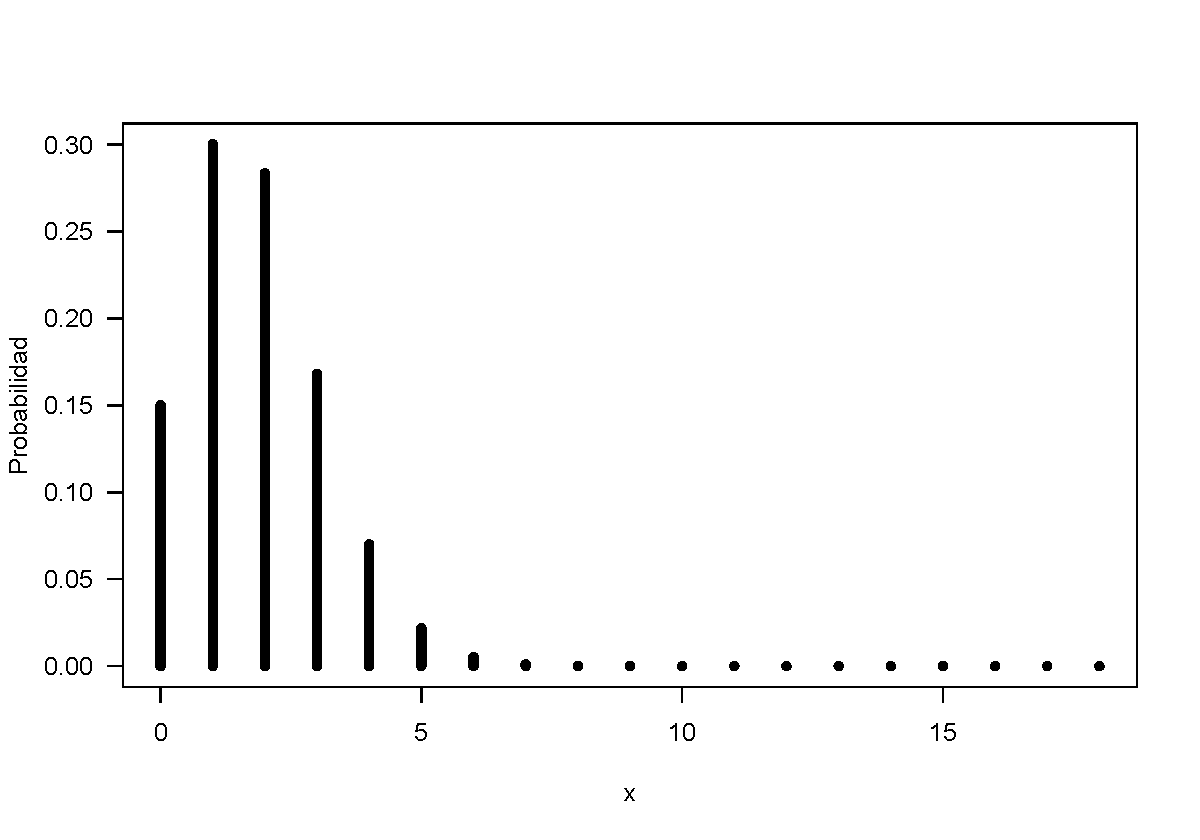
\includegraphics{Manual_de_R_files/figure-latex/binom1-1.pdf}
\caption{\label{fig:binom1}Función de masa de probabilidad para una
\(Binomial(n=18, p=0.1)\).}
\end{figure}

En la Figura \ref{fig:binom1} se muestra la función de masa de
probabilidad para la \(Binomial(n=18, p=0.1)\), de esta figura se
observa claramente que la mayor parte de la probabilidad está
concentrada para valores pequeños de \(X\) debido a que la probabilidad
de éxito individual es \(p=0.10\). Valores de \(X \geq 7\) tienen una
probabilidad muy pequeña y es por eso que las longitudes de sus barras
son muy cortas.

\begin{enumerate}
\def\labelenumi{\arabic{enumi})}
\setcounter{enumi}{4}
\tightlist
\item
  Generar con 100 de una distribución \(Binomial(n=18, p=0.1)\) y luego
  calcular las frecuencias muestrales y compararlas con las
  probabilidades teóricas.
\end{enumerate}

La muestra aleatoria se obtiene con la función \texttt{rbinom} y los
resultados se almacenan en el objeto \texttt{m}, por último se construye
la tabla de frecuencias relativas, a continuación el código usado.

\begin{Shaded}
\begin{Highlighting}[]
\NormalTok{m <-}\StringTok{ }\KeywordTok{rbinom}\NormalTok{(}\DataTypeTok{n=}\DecValTok{100}\NormalTok{, }\DataTypeTok{size=}\DecValTok{18}\NormalTok{, }\DataTypeTok{prob=}\FloatTok{0.1}\NormalTok{)}
\NormalTok{m  }\CommentTok{# Para ver lo que hay dentro de m}
\end{Highlighting}
\end{Shaded}

\begin{verbatim}
##   [1] 1 1 3 5 1 1 2 2 0 3 1 0 2 0 3 2 0 3 3 0 2 1 4 1 0
##  [26] 4 4 3 1 1 3 2 2 4 1 2 0 2 4 1 3 2 1 2 1 3 1 1 1 3
##  [51] 2 1 1 3 3 2 0 1 1 1 2 1 2 0 3 2 3 3 3 6 2 2 1 2 3
##  [76] 3 3 1 3 3 4 2 3 0 2 1 3 3 1 1 2 1 2 1 1 0 3 3 1 3
\end{verbatim}

\begin{Shaded}
\begin{Highlighting}[]
\KeywordTok{prop.table}\NormalTok{(}\KeywordTok{table}\NormalTok{(m))  }\CommentTok{# Tabla de frecuencia relativa}
\end{Highlighting}
\end{Shaded}

\begin{verbatim}
## m
##    0    1    2    3    4    5    6 
## 0.11 0.31 0.23 0.27 0.06 0.01 0.01
\end{verbatim}

A pesar de ser una muestra aleatoria de sólo 100 observaciones, se
observa que las frecuencias relativas obtenidas son muy cercanas a las
mostradas en la Figura \ref{fig:binom1}.

\subsection*{Ejemplo geométrica}\label{ejemplo-geometrica}


En una línea de producción de bombillos se sabe que sólo el 1\% de los
bombillos son defectuosos. Una máquina automática toma un bombillo y lo
prueba, si el bombillo enciende, se siguen probando los bombillos hasta
que se encuentre \textbf{un} bombillo defectuoso, ahí se para la línea
de producción y se toman los correctivos necesarios para mejorar el
proceso.

\begin{enumerate}
\def\labelenumi{\arabic{enumi})}
\tightlist
\item
  Calcular la probabilidad de que se necesiten probar 125 bombillos para
  encontrar el primer bombillo defectuoso.
\end{enumerate}

En la distribución geométrica, la variable \(X\) representa el número de
fracasos antes de encontrar el único éxito, por lo tanto, en este caso
el interés es calcular \(P(X=124)\). La instrucción para obtener esta
probabiliad es la siguiente.

\begin{Shaded}
\begin{Highlighting}[]
\KeywordTok{dgeom}\NormalTok{(}\DataTypeTok{x=}\DecValTok{124}\NormalTok{, }\DataTypeTok{prob=}\FloatTok{0.01}\NormalTok{)}
\end{Highlighting}
\end{Shaded}

\begin{verbatim}
## [1] 0.002876
\end{verbatim}

\begin{enumerate}
\def\labelenumi{\arabic{enumi})}
\setcounter{enumi}{1}
\tightlist
\item
  Calcular \(P(X \leq 8)\).
\end{enumerate}

En este caso interesa \(P(X \leq 50)\) lo que equivale a \(F(8)\), la
instrucción para obtener la probabilidad es la siguiente.

\begin{Shaded}
\begin{Highlighting}[]
\KeywordTok{pgeom}\NormalTok{(}\DataTypeTok{q=}\DecValTok{50}\NormalTok{, }\DataTypeTok{prob=}\FloatTok{0.01}\NormalTok{)}
\end{Highlighting}
\end{Shaded}

\begin{verbatim}
## [1] 0.401
\end{verbatim}

\begin{enumerate}
\def\labelenumi{\arabic{enumi})}
\setcounter{enumi}{2}
\tightlist
\item
  Encontrar el cuantil \(q\) tal que \(P(X \leq q) = 0.40\).
\end{enumerate}

En este caso interesa encontrar el cuantil \(q\) que cumpla la condición
de que hasta \(q\) esté el 40\% de las observaciones, por esa razón se
usa la función \texttt{qgeom} como se muestra a continuación.

\begin{Shaded}
\begin{Highlighting}[]
\KeywordTok{qgeom}\NormalTok{(}\DataTypeTok{p=}\FloatTok{0.4}\NormalTok{, }\DataTypeTok{prob=}\FloatTok{0.01}\NormalTok{)}
\end{Highlighting}
\end{Shaded}

\begin{verbatim}
## [1] 50
\end{verbatim}

\BeginKnitrBlock{rmdnote}
Note que las funciones \texttt{pxxx} y \texttt{qxxx} están relacionadas,
\texttt{pxxx} entrega la probabilidad hasta el cuantil \(q\) mientras
\texttt{qxxx} entrega el cuantil en el que se acumula \(p\)
probabilidad.
\EndKnitrBlock{rmdnote}

\subsection*{Ejemplo binomial negativa}\label{ejemplo-binomial-negativa}


Una familia desea tener hijos hasta conseguir \textbf{2 niñas}, la
probabilidad individual de obtener una niña es 0.5 y se supone que todos
los nacimientos son individuales, es decir, un sólo bebé.

\begin{enumerate}
\def\labelenumi{\arabic{enumi})}
\tightlist
\item
  Calcular la probabilidad de que se necesiten 4 hijos, es decir, 4
  nacimientos para consguir las dos niñas.
\end{enumerate}

En este problema se tiene una distribución binomial negativa con \(r=2\)
niñas, los éxitos deseados por la familia. La variable \(X\) representa
los fracasos, es decir los niños, hasta que se obtienen los éxitos
\(r=2\) deseados.

En este caso lo que interesa es \(P(\text{familia tenga 4})\), en otras
palabras interesa \(P(X=2)\), la instrucción para calcular la
probabilidad es la siguiente.

\begin{Shaded}
\begin{Highlighting}[]
\KeywordTok{dnbinom}\NormalTok{(}\DataTypeTok{x=}\DecValTok{2}\NormalTok{, }\DataTypeTok{size=}\DecValTok{2}\NormalTok{, }\DataTypeTok{prob=}\FloatTok{0.5}\NormalTok{)}
\end{Highlighting}
\end{Shaded}

\begin{verbatim}
## [1] 0.1875
\end{verbatim}

\begin{enumerate}
\def\labelenumi{\arabic{enumi})}
\setcounter{enumi}{1}
\tightlist
\item
  Calcular \(P(\text{familia tenga al menos 4 hijos})\).
\end{enumerate}

Aquí interesa calcular \(P(X \geq 2)=P(X=2)+P(X=3)+\ldots\), como esta
probabilidad va hasta infinito, se debe usar el complemento así:

\[P(X \geq 2) = 1 - [P(X=0)+P(X=1)]\] y para obtener la probabilidad
solicitada se puede usar la función \texttt{dnbinom} de la siguiente
manera.

\begin{Shaded}
\begin{Highlighting}[]
\DecValTok{1} \NormalTok{-}\StringTok{ }\KeywordTok{sum}\NormalTok{(}\KeywordTok{dnbinom}\NormalTok{(}\DataTypeTok{x=}\DecValTok{0}\NormalTok{:}\DecValTok{1}\NormalTok{, }\DataTypeTok{size=}\DecValTok{2}\NormalTok{, }\DataTypeTok{prob=}\FloatTok{0.5}\NormalTok{))}
\end{Highlighting}
\end{Shaded}

\begin{verbatim}
## [1] 0.5
\end{verbatim}

Otra forma para obtener la probabilidad solicitada es por medio de la
función \texttt{pnbinom} de la siguiente manera.

\begin{Shaded}
\begin{Highlighting}[]
\DecValTok{1} \NormalTok{-}\StringTok{ }\KeywordTok{pnbinom}\NormalTok{(}\DataTypeTok{q=}\DecValTok{1}\NormalTok{, }\DataTypeTok{size=}\DecValTok{2}\NormalTok{, }\DataTypeTok{prob=}\FloatTok{0.5}\NormalTok{)}
\end{Highlighting}
\end{Shaded}

\begin{verbatim}
## [1] 0.5
\end{verbatim}

\subsection*{Ejemplo hipergeométrica}\label{ejemplo-hipergeometrica}


Un lote de partes para ensamblar en una empresa está formado por 100
elementos del proveedor A y 200 elementos del proveedor B. Se selecciona
una muestra de 4 partes al azar sin reemplazo de las 300 para una
revisión de calidad.

\begin{enumerate}
\def\labelenumi{\arabic{enumi})}
\tightlist
\item
  Calcular la probabilidad de que todas las 4 partes de la muestra sean
  del proveedor A.
\end{enumerate}

Aquí se tiene una situación que se puede modelar por medio de una
distribución hipergeométrica con \(m=100\) éxitos en la población,
\(n=200\) fracasos en la población y \(k=4\) el tamaño de la muestra. El
objetivo es calcular \(P(X=4)\), para obtener esta probabilidad se usa
la siguiente instrucción.

\begin{Shaded}
\begin{Highlighting}[]
\KeywordTok{dhyper}\NormalTok{(}\DataTypeTok{x=}\DecValTok{4}\NormalTok{, }\DataTypeTok{m=}\DecValTok{100}\NormalTok{, }\DataTypeTok{k=}\DecValTok{4}\NormalTok{, }\DataTypeTok{n=}\DecValTok{200}\NormalTok{)}
\end{Highlighting}
\end{Shaded}

\begin{verbatim}
## [1] 0.01185
\end{verbatim}

\begin{enumerate}
\def\labelenumi{\arabic{enumi})}
\setcounter{enumi}{1}
\tightlist
\item
  Calcular la probabilidad de que dos o más de las partes sean del
  proveedor A.
\end{enumerate}

Aquí interesa \(P(X \geq 2)\), la instrucción para obtener esta
probabilidad es.

\begin{Shaded}
\begin{Highlighting}[]
\KeywordTok{sum}\NormalTok{(}\KeywordTok{dhyper}\NormalTok{(}\DataTypeTok{x=}\DecValTok{2}\NormalTok{:}\DecValTok{4}\NormalTok{, }\DataTypeTok{m=}\DecValTok{100}\NormalTok{, }\DataTypeTok{k=}\DecValTok{4}\NormalTok{, }\DataTypeTok{n=}\DecValTok{200}\NormalTok{))}
\end{Highlighting}
\end{Shaded}

\begin{verbatim}
## [1] 0.4074
\end{verbatim}

\subsection*{Ejemplo Poisson}\label{ejemplo-poisson}


En una editorial se asume que todo libro de 250 páginas tiene en
promedio 50 errores.

\begin{enumerate}
\def\labelenumi{\arabic{enumi})}
\tightlist
\item
  Encuentre la probabilidad de que en una página cualquiera no se
  encuentren errores.
\end{enumerate}

Este es un problema de distribución Poisson con tasa promedio de éxitos
dada por:

\[\lambda=\frac{50 \quad errores}{libro}=\frac{0.2 \quad errores}{pagina}\]
El objetivo es calcular \(P(X=0)\), para obtener esta probabilidad de
usa la siguiente instrucción.

\begin{Shaded}
\begin{Highlighting}[]
\KeywordTok{dpois}\NormalTok{(}\DataTypeTok{x=}\DecValTok{0}\NormalTok{, }\DataTypeTok{lambda=}\FloatTok{0.2}\NormalTok{)}
\end{Highlighting}
\end{Shaded}

\begin{verbatim}
## [1] 0.8187
\end{verbatim}

Así \(P(X=0)=0.8187\).

\section{Distribuciones discretas
generales}\label{distribuciones-discretas-generales}

En la práctica nos podemos encontramos con variables aleatorias
discretas que no se ajustan a una de las distribuciones mostradas
anteriormente, en esos casos, es posible manejar ese tipo de variables
por medio de unas funciones básicas de \proglang{R} como se muestra en
el siguiente ejemplo.

\subsection*{Ejemplo}\label{ejemplo-42}


El cangrejo de herradura hembra se caracteriza porque a su caparazón se
adhieren los machos de la misma especie, en la Figura \ref{fig:crab} se
muestra una fotografía de este cangrejo. Los investigadores están
interesado en determinar cual es el patrón de variación del número de
machos sobre cada hembra, para esto, se recolectó una muestra de hembras
a las cuales se les observó el color, la condición de la espina, el peso
en kilogramos, el ancho del caparazón en centímetros y el número de
satélites o machos sobre el caparazón, la base de datos está disponible
en el siguiente
\href{https://raw.githubusercontent.com/fhernanb/datos/master/crab}{enlace}.

\begin{figure}

{\centering 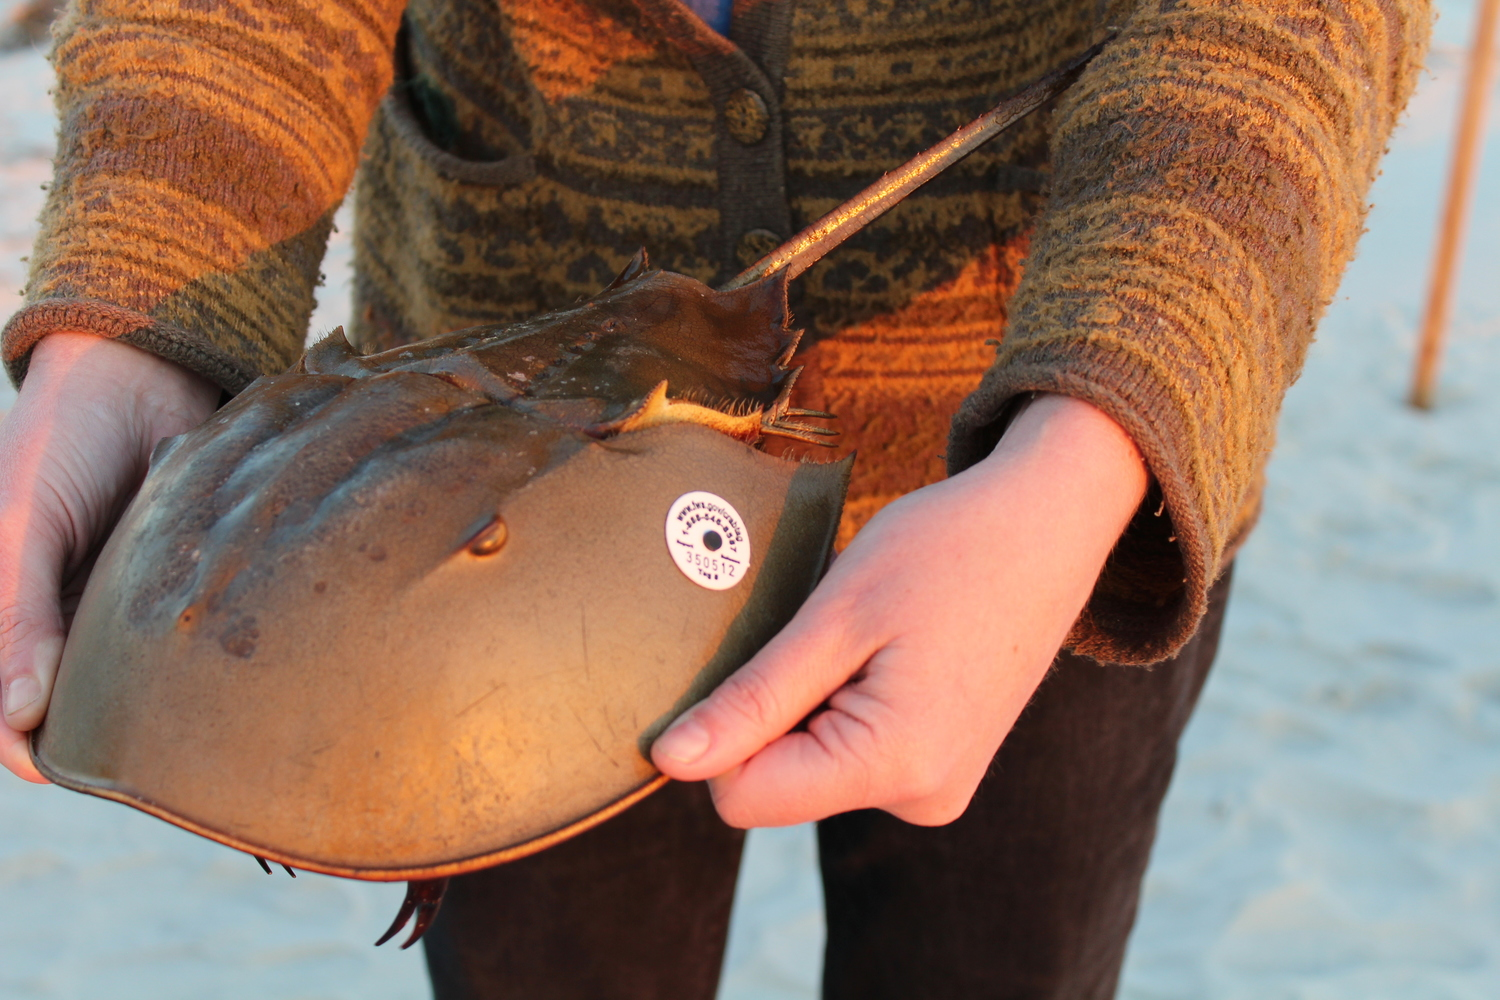
\includegraphics{images/crab} 

}

\caption{Fotografía del cangreo de herradura, tomada de http://sccoastalresources.com/home/2016/6/21/a-night-of-horseshoe-crab-tagging.}\label{fig:crab}
\end{figure}

\begin{enumerate}
\def\labelenumi{\arabic{enumi})}
\tightlist
\item
  Encontrar la distribución de probabilidad para la variable \texttt{Sa}
  que corresponde al número de machos sobre el caparazón de cada hembra.
\end{enumerate}

Primero se debe leer la base de datos usando la url suministrada y luego
se construye la tabla de frecuencia relativa y se almacena en el objeto
\texttt{t1}.

\begin{Shaded}
\begin{Highlighting}[]
\NormalTok{url <-}\StringTok{ 'https://raw.githubusercontent.com/fhernanb/datos/master/crab'}
\NormalTok{crab <-}\StringTok{ }\KeywordTok{read.table}\NormalTok{(}\DataTypeTok{file=}\NormalTok{url, }\DataTypeTok{header=}\NormalTok{T)}

\NormalTok{t1 <-}\StringTok{ }\KeywordTok{prop.table}\NormalTok{(}\KeywordTok{table}\NormalTok{(crab$Sa))}
\NormalTok{t1}
\end{Highlighting}
\end{Shaded}

\begin{verbatim}
## 
##       0       1       2       3       4       5 
## 0.35838 0.09249 0.05202 0.10983 0.10983 0.08671 
##       6       7       8       9      10      11 
## 0.07514 0.02312 0.03468 0.01734 0.01734 0.00578 
##      12      14      15 
## 0.00578 0.00578 0.00578
\end{verbatim}

La anterior tabla de frecuencias relativas se puede representar
gráficamente usando el siguiente código.

\begin{Shaded}
\begin{Highlighting}[]
\KeywordTok{plot}\NormalTok{(t1, }\DataTypeTok{las=}\DecValTok{1}\NormalTok{, }\DataTypeTok{lwd=}\DecValTok{5}\NormalTok{, }\DataTypeTok{xlab=}\StringTok{'Número de satélites'}\NormalTok{,}
     \DataTypeTok{ylab=}\StringTok{'Proporción'}\NormalTok{)}
\end{Highlighting}
\end{Shaded}

\begin{figure}[htbp]
\centering
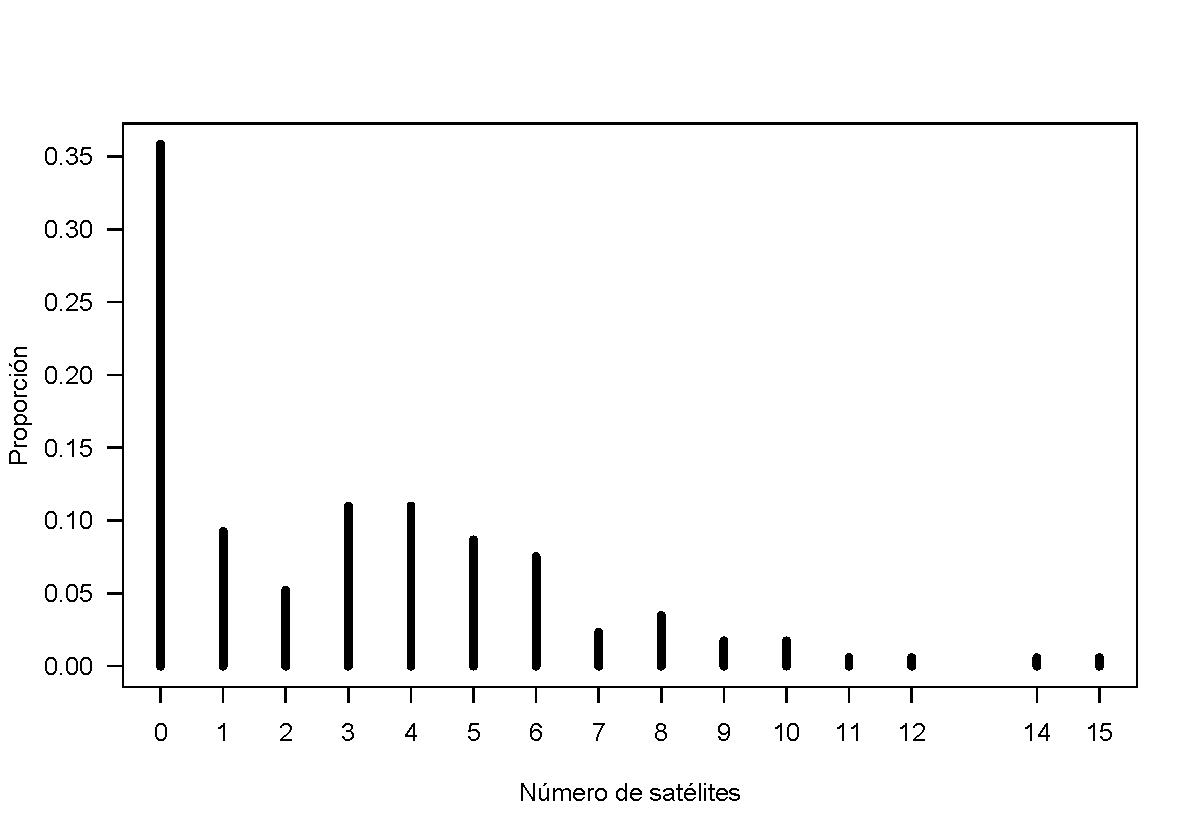
\includegraphics{Manual_de_R_files/figure-latex/pmfcrab-1.pdf}
\caption{\label{fig:pmfcrab}Función de masa de probabilidad para el número
de satélites por hembra.}
\end{figure}

\begin{enumerate}
\def\labelenumi{\arabic{enumi})}
\setcounter{enumi}{1}
\tightlist
\item
  Sea \(X\) la variable número de satélites por hembra, construir la
  función \(F(x)\).
\end{enumerate}

Para construir \(F(x)\) se utiliza la función \texttt{ecdf} o
\emph{empirical cumulative density function}, a esta función le debe
ingresar el vector con la información de la variable cuantitativa, a
continuación del código usado. En la Figura \ref{fig:Fcrab} se muestra
la función de distribución acumulada para para el número de satélites
por hembra.

\begin{Shaded}
\begin{Highlighting}[]
\NormalTok{F <-}\StringTok{ }\KeywordTok{ecdf}\NormalTok{(crab$Sa)}
\KeywordTok{plot}\NormalTok{(F, }\DataTypeTok{las=}\DecValTok{1}\NormalTok{, }\DataTypeTok{main=}\StringTok{''}\NormalTok{)}
\end{Highlighting}
\end{Shaded}

\begin{figure}[htbp]
\centering
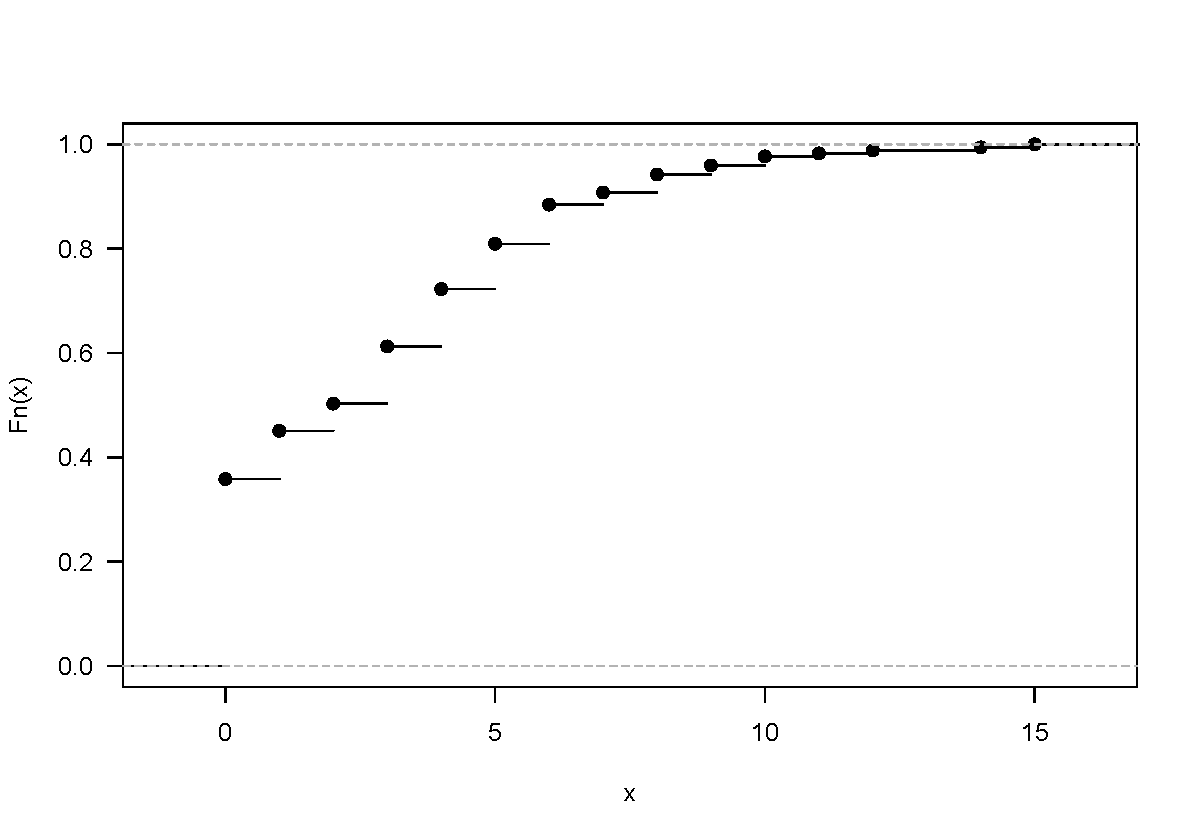
\includegraphics{Manual_de_R_files/figure-latex/Fcrab-1.pdf}
\caption{\label{fig:Fcrab}Función de distribución acumulada para el número
de satélites por hembra.}
\end{figure}

\begin{enumerate}
\def\labelenumi{\arabic{enumi})}
\setcounter{enumi}{2}
\tightlist
\item
  Calcular \(P(X \leq 9)\).
\end{enumerate}

Para obtener esta probabilidad se usa el objeto \texttt{F} que es en
realidad una función, a continuación la instrucción usada.

\begin{Shaded}
\begin{Highlighting}[]
\KeywordTok{F}\NormalTok{(}\DecValTok{9}\NormalTok{)}
\end{Highlighting}
\end{Shaded}

\begin{verbatim}
## [1] 0.9595
\end{verbatim}

Así \(P(X \leq 9)=0.9595\).

\begin{enumerate}
\def\labelenumi{\arabic{enumi})}
\setcounter{enumi}{3}
\tightlist
\item
  Calcular \(P(X > 4)\).
\end{enumerate}

Para obtener esta probabilidad se usa el hecho de que
\(P(X > 4) = 1 - P(X \leq 4)\), así la instrucción a usar es.

\begin{Shaded}
\begin{Highlighting}[]
\DecValTok{1} \NormalTok{-}\StringTok{ }\KeywordTok{F}\NormalTok{(}\DecValTok{4}\NormalTok{)}
\end{Highlighting}
\end{Shaded}

\begin{verbatim}
## [1] 0.2775
\end{verbatim}

Por lo tanto \(P(X > 4)=0.2775\).

\begin{enumerate}
\def\labelenumi{\arabic{enumi})}
\setcounter{enumi}{4}
\tightlist
\item
  Suponga que el grupo 1 está formado por las hembras cuyo ancho de
  caparazón es menor o igual al ancho mediano, el grupo 2 está formado
  por las demás hembras. ¿Será \(F(x)\) diferente para los dos grupos?
\end{enumerate}

Para realizar esto vamos a particionar el vector \texttt{Sa} en los dos
grupos de acuerdo a la nueva variable \texttt{grupo} creada como se
muestra a continuacion.

\begin{Shaded}
\begin{Highlighting}[]
\NormalTok{grupo <-}\StringTok{ }\KeywordTok{ifelse}\NormalTok{(crab$Wt <=}\StringTok{ }\KeywordTok{median}\NormalTok{(crab$Wt), }\StringTok{'Grupo 1'}\NormalTok{, }\StringTok{'Grupo 2'}\NormalTok{)}
\NormalTok{x <-}\StringTok{ }\KeywordTok{split}\NormalTok{(}\DataTypeTok{x=}\NormalTok{crab$Sa, }\DataTypeTok{f=}\NormalTok{grupo)}
\end{Highlighting}
\end{Shaded}

El objeto \texttt{x} es una lista y para acceder a los vectores allí
almacenados usamos dos corchetes \texttt{{[}{[}{]}{]}}, uno dentro del
otro. Luego para calcular \(F(x)\) para los dos grupos se procede así:

\begin{Shaded}
\begin{Highlighting}[]
\NormalTok{F1 <-}\StringTok{ }\KeywordTok{ecdf}\NormalTok{(x[[}\DecValTok{1}\NormalTok{]])}
\NormalTok{F2 <-}\StringTok{ }\KeywordTok{ecdf}\NormalTok{(x[[}\DecValTok{2}\NormalTok{]])}
\end{Highlighting}
\end{Shaded}

Para obtener las dos \(F(x)\) en la misma figura se usa el código
siguiente.

\begin{Shaded}
\begin{Highlighting}[]
\KeywordTok{plot}\NormalTok{(F1, }\DataTypeTok{col=}\StringTok{'blue'}\NormalTok{, }\DataTypeTok{main=}\StringTok{''}\NormalTok{, }\DataTypeTok{las=}\DecValTok{1}\NormalTok{)}
\KeywordTok{plot}\NormalTok{(F2, }\DataTypeTok{col=}\StringTok{'red'}\NormalTok{, }\DataTypeTok{add=}\NormalTok{T)}
\KeywordTok{legend}\NormalTok{(}\StringTok{'bottomright'}\NormalTok{, }\DataTypeTok{legend=}\KeywordTok{c}\NormalTok{(}\StringTok{'Grupo 1'}\NormalTok{, }\StringTok{'Grupo 2'}\NormalTok{),}
       \DataTypeTok{col=}\KeywordTok{c}\NormalTok{(}\StringTok{'blue'}\NormalTok{, }\StringTok{'red'}\NormalTok{), }\DataTypeTok{lwd=}\DecValTok{1}\NormalTok{)}
\end{Highlighting}
\end{Shaded}

\begin{figure}[htbp]
\centering
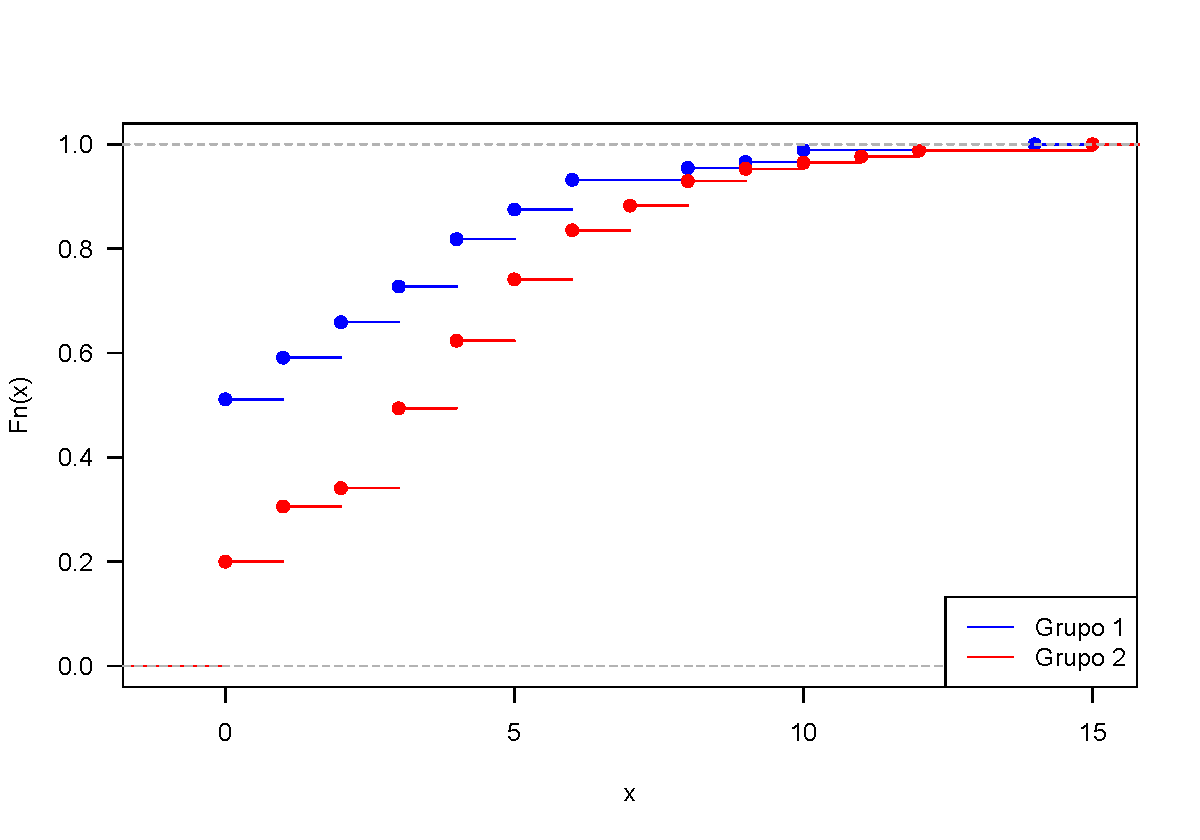
\includegraphics{Manual_de_R_files/figure-latex/Fcrabs-1.pdf}
\caption{\label{fig:Fcrabs}Función de distribución acumulada para el número
de satélites por hembra diferenciando por grupo.}
\end{figure}

En la Figura \ref{fig:Fcrabs} se muestran las dos \(F(x)\), en color
azul para el grupo 1 y en color rojo para el grupo 2. Se observa
claramente que las curvas son diferentes antes de \(x=9\). El hecho de
que la curva azul esté por encima de la roja para valores menores de 9,
es decir, \(F_1(x) \geq F_2(x)\), indica que las hembras del grupo 1
tienden a tener menos satélites que las del grupo 2, esto es coherente
ya que las del grupo 2 son más grandes en su caparazón.

\chapter{Distribuciones continuas}\label{distribuciones-continuas}

En este capítulo se mostrarán las funciones de \proglang{R} para
distribuciones continuas.

\section{Funciones disponibles para distribuciones
continuas}\label{funciones-disponibles-para-distribuciones-continuas}

Para cada distribución continua se tienen 4 funciones, a continuación el
listado de las funciones y su utilidad.

\begin{Shaded}
\begin{Highlighting}[]
\KeywordTok{dxxx}\NormalTok{(x, ...)  }\CommentTok{# Función de densidad de probabilidad, f(x)}
\KeywordTok{pxxx}\NormalTok{(q, ...)  }\CommentTok{# Función de distribución acumulada hasta q, F(x)}
\KeywordTok{qxxx}\NormalTok{(p, ...)  }\CommentTok{# Cuantil para el cual P(X <= q) = p}
\KeywordTok{rxxx}\NormalTok{(n, ...)  }\CommentTok{# Generador de números aleatorios.}
\end{Highlighting}
\end{Shaded}

En el lugar de las letras \texttt{xxx} se de debe colocar el nombre de
la distribución en \proglang{R}, a continuación el listado de nombres
disponibles para las 11 distribuciones continuas básicas.

\begin{Shaded}
\begin{Highlighting}[]
\NormalTok{beta     }\CommentTok{# Beta}
\NormalTok{cauchy   }\CommentTok{# Cauchy}
\NormalTok{chisq    }\CommentTok{# Chi-cuadrada}
\NormalTok{exp      }\CommentTok{# Exponencial}
\NormalTok{f        }\CommentTok{# F}
\NormalTok{gamma    }\CommentTok{# Gama}
\NormalTok{lnorm    }\CommentTok{# log-normal}
\NormalTok{norm     }\CommentTok{# normal}
\NormalTok{t        }\CommentTok{# t-student}
\NormalTok{unif     }\CommentTok{# Uniforme}
\NormalTok{weibull  }\CommentTok{# Weibull}
\end{Highlighting}
\end{Shaded}

Combinando las funciones y los nombres se tiene un total de 44
funciones, por ejemplo, para obtener la función de densidad de
probabilidad \(f(x)\) de una normal se usa la función \texttt{dnorm(\ )}
y para obtener la función acumulada \(F(x)\) de una Beta se usa la
función \texttt{pbeta(\ )}.

\subsection*{Ejemplo beta}\label{ejemplo-beta}


Considere que una variable aleatoria \(X\) se distribuye beta con
parámetros \(a=2\) y \(b=5\).

\begin{enumerate}
\def\labelenumi{\arabic{enumi})}
\tightlist
\item
  Dibuje la densidad de la distribución.
\end{enumerate}

La función \texttt{dbeta} sirve para obtener la altura de la curva de
una distribución beta y combinándola con la función \texttt{curve} se
puede dibujar la densidad solicitada. En la Figura \ref{fig:beta1} se
presenta la densidad, observe que para la combinación de parámetros
\(a=2\) y \(b=5\) la distribución es sesgada a la derecha.

\begin{Shaded}
\begin{Highlighting}[]
\KeywordTok{curve}\NormalTok{(}\KeywordTok{dbeta}\NormalTok{(x, }\DataTypeTok{shape1=}\DecValTok{2}\NormalTok{, }\DataTypeTok{shape2=}\DecValTok{5}\NormalTok{), }\DataTypeTok{lwd=}\DecValTok{3}\NormalTok{, }\DataTypeTok{las=}\DecValTok{1}\NormalTok{,}
      \DataTypeTok{ylab=}\StringTok{'Densidad'}\NormalTok{)}
\end{Highlighting}
\end{Shaded}

\begin{figure}[htbp]
\centering
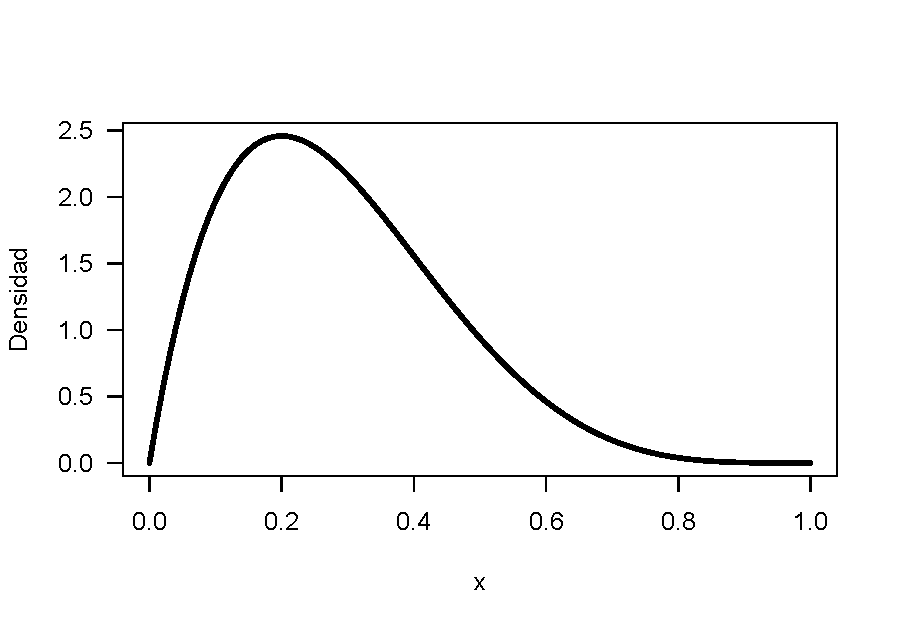
\includegraphics{Manual_de_R_files/figure-latex/beta1-1.pdf}
\caption{\label{fig:beta1}Función de densidad para una \(Beta(2, 5)\).}
\end{figure}

\begin{enumerate}
\def\labelenumi{\arabic{enumi})}
\setcounter{enumi}{1}
\tightlist
\item
  Calcular \(P(0.3 \leq X \leq 0.7)\).
\end{enumerate}

Para obtener la probabilidad o área bajo la densidad se puede usar la
función \texttt{integrate}, los límites de la integral se ingresan por
medio de los parámetros \texttt{lower} y \texttt{upper}. Si la función a
integrar tiene parámetros adicionales como en este caso, éstos
parámetros se ingresan luego de los límites de la integral. A
continuación el código necesario para obtener la probabiliad solicitada.

\begin{Shaded}
\begin{Highlighting}[]
\KeywordTok{integrate}\NormalTok{(}\DataTypeTok{f=}\NormalTok{dbeta, }\DataTypeTok{lower=}\FloatTok{0.3}\NormalTok{, }\DataTypeTok{upper=}\FloatTok{0.7}\NormalTok{,}
          \DataTypeTok{shape1=}\DecValTok{2}\NormalTok{, }\DataTypeTok{shape2=}\DecValTok{5}\NormalTok{)}
\end{Highlighting}
\end{Shaded}

\begin{verbatim}
## 0.4092 with absolute error < 4.5e-15
\end{verbatim}

Otra forma de obtener la probabilidad solicitada es restando de
\(F(x_{max})\) la probabilidad \(F(x_{min})\). Las probabilidades
acumuladas hasta un valor dado se obtienen con la función
\texttt{pbeta}, a continuación el código necesario.

\begin{Shaded}
\begin{Highlighting}[]
\KeywordTok{pbeta}\NormalTok{(}\DataTypeTok{q=}\FloatTok{0.7}\NormalTok{, }\DataTypeTok{shape1=}\DecValTok{2}\NormalTok{, }\DataTypeTok{shape2=}\DecValTok{5}\NormalTok{) -}\StringTok{ }\KeywordTok{pbeta}\NormalTok{(}\DataTypeTok{q=}\FloatTok{0.3}\NormalTok{, }\DataTypeTok{shape1=}\DecValTok{2}\NormalTok{, }\DataTypeTok{shape2=}\DecValTok{5}\NormalTok{)}
\end{Highlighting}
\end{Shaded}

\begin{verbatim}
## [1] 0.4092
\end{verbatim}

De ambas formas se obtiene que \(P(0.3 \leq X \leq 0.7)=0.4092\).

\BeginKnitrBlock{rmdnote}
Recuerde que para distribuciones continuas

\[ P(a < X < b) = P(a \leq X < b) = P(a < X \leq b) = P(a \leq X \leq b)\]
\EndKnitrBlock{rmdnote}

\subsection*{Ejemplo normal estándar}\label{ejemplo-normal-estandar}


Suponga que la variable aleatoria \(Z\) se distribuye normal estándar,
es decir, \(Z \sim N(0, 1)\).

\begin{enumerate}
\def\labelenumi{\arabic{enumi})}
\tightlist
\item
  Calcular \(P(Z < 1.45)\).
\end{enumerate}

Para calcular la probabilidad acumulada hasta un punto dado se usa la
función \texttt{pnorm} y se evalúa en el cuantil indicado, a
continuación el código usado.

\begin{Shaded}
\begin{Highlighting}[]
\KeywordTok{pnorm}\NormalTok{(}\DataTypeTok{q=}\FloatTok{1.45}\NormalTok{)}
\end{Highlighting}
\end{Shaded}

\begin{verbatim}
## [1] 0.9265
\end{verbatim}

En la Figura \ref{fig:norm1} se muestra el área sombreada
correspondiente a \(P(Z < 1.45)\).

\begin{enumerate}
\def\labelenumi{\arabic{enumi})}
\setcounter{enumi}{1}
\tightlist
\item
  Calcular \(P(Z > -0.37)\).
\end{enumerate}

Para calcular la probabilidad solicitada se usa nuevamente la función
\texttt{pnorm} evaluada en el cuantil dado. Como el evento de interés es
\(Z > -0.37\), la probabilidad solicitada se obtiene como
\texttt{1\ -\ pnorm(q=-0.37)}, esto debido a que por defecto las
probabilidades entregadas por la función \texttt{pxxx} son siempre a
izquierda. A continuación el código usado.

\begin{Shaded}
\begin{Highlighting}[]
\DecValTok{1} \NormalTok{-}\StringTok{ }\KeywordTok{pnorm}\NormalTok{(}\DataTypeTok{q=}\NormalTok{-}\FloatTok{0.37}\NormalTok{)}
\end{Highlighting}
\end{Shaded}

\begin{verbatim}
## [1] 0.6443
\end{verbatim}

En la Figura \ref{fig:norm1} se muestra el área sombreada
correspondiente a \(P(Z > -0.37)\).

Otra forma para obtener la probabilidad solicitada sin hacer la resta es
usar el parámetro \texttt{lower.tail} para indicar que interesa la
probabilidad a la derecha del cuantil dado, a continuación un código
alternativo para obtener la misma probabilidad.

\begin{Shaded}
\begin{Highlighting}[]
\KeywordTok{pnorm}\NormalTok{(}\DataTypeTok{q=}\NormalTok{-}\FloatTok{0.37}\NormalTok{, }\DataTypeTok{lower.tail=}\OtherTok{FALSE}\NormalTok{)}
\end{Highlighting}
\end{Shaded}

\begin{verbatim}
## [1] 0.6443
\end{verbatim}

\begin{enumerate}
\def\labelenumi{\arabic{enumi})}
\setcounter{enumi}{2}
\tightlist
\item
  Calcular \(P(-1.56 < Z < 2.58)\).
\end{enumerate}

Para calcular la probabilidad solicitada se obtiene la probabilidad
acumulada hasta 2.58 y de ella se resta lo acumulado hasta -1.56, a
continuación el código usado.

\begin{Shaded}
\begin{Highlighting}[]
\KeywordTok{pnorm}\NormalTok{(}\DataTypeTok{q=}\FloatTok{2.58}\NormalTok{) -}\StringTok{ }\KeywordTok{pnorm}\NormalTok{(-}\FloatTok{1.56}\NormalTok{)}
\end{Highlighting}
\end{Shaded}

\begin{verbatim}
## [1] 0.9357
\end{verbatim}

En la Figura \ref{fig:norm1} se muestra el área sombreada
correspondiente a \(P(-1.56 < Z < 2.58)\).

\begin{enumerate}
\def\labelenumi{\arabic{enumi})}
\setcounter{enumi}{3}
\tightlist
\item
  Calcular el cuantil \(q\) para el cual se cumple que \(P(Z<q)=0.95\).
\end{enumerate}

Para calcular el cuantil en el cual se cumple que \(P(Z<q)=0.95\) se usa
la función \texttt{qnorm}, a continuación el código usado.

\begin{Shaded}
\begin{Highlighting}[]
\KeywordTok{qnorm}\NormalTok{(}\DataTypeTok{p=}\FloatTok{0.95}\NormalTok{) }
\end{Highlighting}
\end{Shaded}

\begin{verbatim}
## [1] 1.645
\end{verbatim}

En la Figura \ref{fig:norm1} se muestra el área sombreada
correspondiente a \(P(Z<q)=0.95\).

\begin{figure}[htbp]
\centering
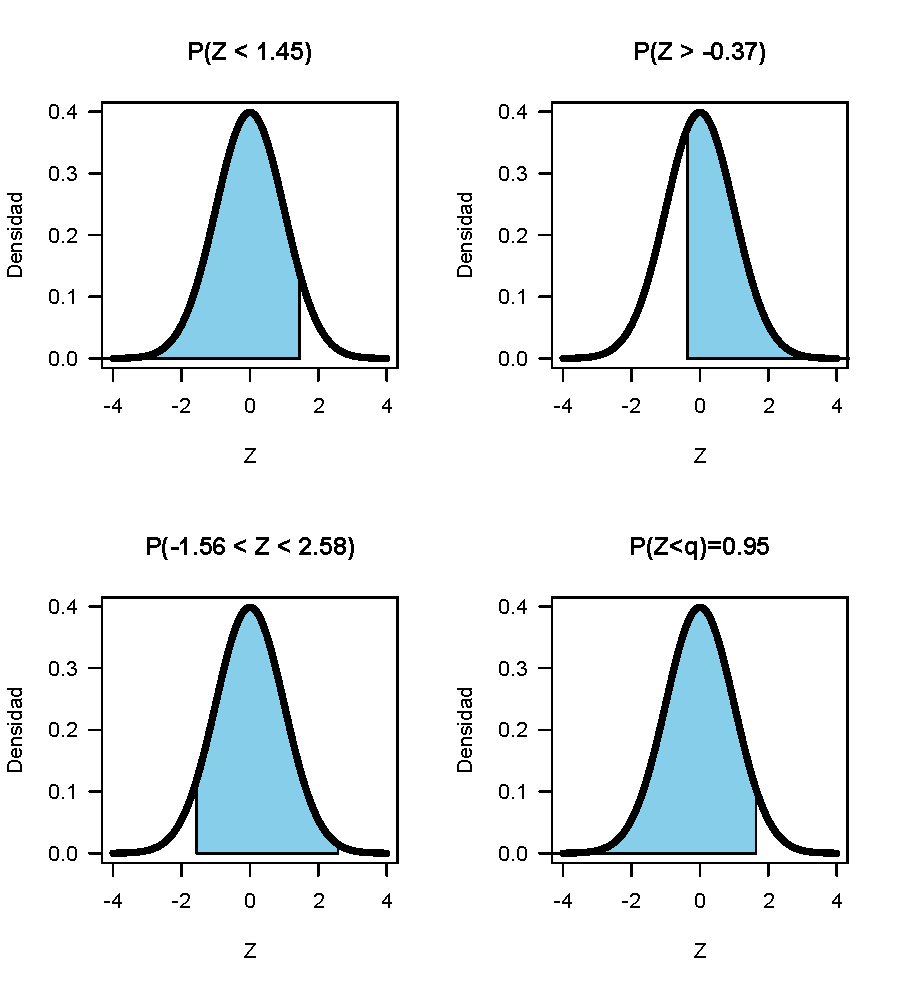
\includegraphics{Manual_de_R_files/figure-latex/norm1-1.pdf}
\caption{\label{fig:norm1}Área sombreada para los ejemplos.}
\end{figure}

\BeginKnitrBlock{rmdtip}
El parámetro \texttt{lower.tail} es muy útil para indicar si estamos
trabajando una cola a izquierda o una cola a derecha.
\EndKnitrBlock{rmdtip}

\subsection*{Ejemplo normal general}\label{ejemplo-normal-general}


Considere un proceso de elaboración de tornillos en una empresa y
suponga que el diámetro de los tornillos sigue una distribución normal
con media de 10 \(mm\) y varianza de 4 \(mm^2\).

\begin{enumerate}
\def\labelenumi{\arabic{enumi})}
\tightlist
\item
  Un tornillo se considera que cumple las especificaciones si su
  diámetro está entre 9 y 11 mm. ¿Qué porcentaje de los tornillos
  cumplen las especificaciones?
\end{enumerate}

Como se solicita probabilidad se debe usar \texttt{pnorm} indicando que
la media es \(\mu=10\) y la desviación de la distribución es
\(\sigma=2\). A continuación el código usado.

\begin{Shaded}
\begin{Highlighting}[]
\KeywordTok{pnorm}\NormalTok{(}\DataTypeTok{q=}\DecValTok{11}\NormalTok{, }\DataTypeTok{mean=}\DecValTok{10}\NormalTok{, }\DataTypeTok{sd=}\DecValTok{2}\NormalTok{) -}\StringTok{ }\KeywordTok{pnorm}\NormalTok{(}\DataTypeTok{q=}\DecValTok{9}\NormalTok{, }\DataTypeTok{mean=}\DecValTok{10}\NormalTok{, }\DataTypeTok{sd=}\DecValTok{2}\NormalTok{)}
\end{Highlighting}
\end{Shaded}

\begin{verbatim}
## [1] 0.3829
\end{verbatim}

\begin{enumerate}
\def\labelenumi{\arabic{enumi})}
\setcounter{enumi}{1}
\tightlist
\item
  Un tornillo con un diámetro mayor a 11 mm se puede reprocesar y
  recuperar. ¿Cuál es el porcentaje de reprocesos en la empresa?
\end{enumerate}

Como se solicita una probabilidad a derecha se usa
\texttt{lower.tail=FALSE} dentro de la función \texttt{pnorm}. A
continuación el código usado.

\begin{Shaded}
\begin{Highlighting}[]
\KeywordTok{pnorm}\NormalTok{(}\DataTypeTok{q=}\DecValTok{11}\NormalTok{, }\DataTypeTok{mean=}\DecValTok{10}\NormalTok{, }\DataTypeTok{sd=}\DecValTok{2}\NormalTok{, }\DataTypeTok{lower.tail=}\OtherTok{FALSE}\NormalTok{)}
\end{Highlighting}
\end{Shaded}

\begin{verbatim}
## [1] 0.3085
\end{verbatim}

\begin{enumerate}
\def\labelenumi{\arabic{enumi})}
\setcounter{enumi}{2}
\tightlist
\item
  El 5\% de los tornillos más delgados no se pueden reprocesar y por lo
  tanto son desperdicio. ¿Qué diámetro debe tener un tornillo para ser
  clasificado como desperdicio?
\end{enumerate}

Aquí interesa encontrar el cuantil tal que \(P(Diametro<q)=0.05\), por
lo tanto se usa la función \texttt{qnorm}. A continuación el código
usado.

\begin{Shaded}
\begin{Highlighting}[]
\KeywordTok{qnorm}\NormalTok{(}\DataTypeTok{p=}\FloatTok{0.05}\NormalTok{, }\DataTypeTok{mean=}\DecValTok{10}\NormalTok{, }\DataTypeTok{sd=}\DecValTok{2}\NormalTok{)}
\end{Highlighting}
\end{Shaded}

\begin{verbatim}
## [1] 6.71
\end{verbatim}

\begin{enumerate}
\def\labelenumi{\arabic{enumi})}
\setcounter{enumi}{3}
\tightlist
\item
  El 10\% de los tornillos más gruesos son considerados como
  sobredimensionados. ¿cuál es el diámetro mínimo de un tornillo para
  que sea considerado como sobredimensionado?
\end{enumerate}

Aquí interesa encontrar el cuantil tal que \(P(Diametro>q)=0.10\), por
lo tanto se usa la función \texttt{qnorm} pero incluyendo
\texttt{lower.tail=FALSE} por ser una cola a derecha. A continuación el
código usado.

\begin{Shaded}
\begin{Highlighting}[]
\KeywordTok{qnorm}\NormalTok{(}\DataTypeTok{p=}\FloatTok{0.10}\NormalTok{, }\DataTypeTok{mean=}\DecValTok{10}\NormalTok{, }\DataTypeTok{sd=}\DecValTok{2}\NormalTok{, }\DataTypeTok{lower.tail=}\OtherTok{FALSE}\NormalTok{)}
\end{Highlighting}
\end{Shaded}

\begin{verbatim}
## [1] 12.56
\end{verbatim}

En la Figura \ref{fig:norm2} se muestran las áreas sombreadas para cada
de las anteriores preguntas.

\begin{figure}[htbp]
\centering
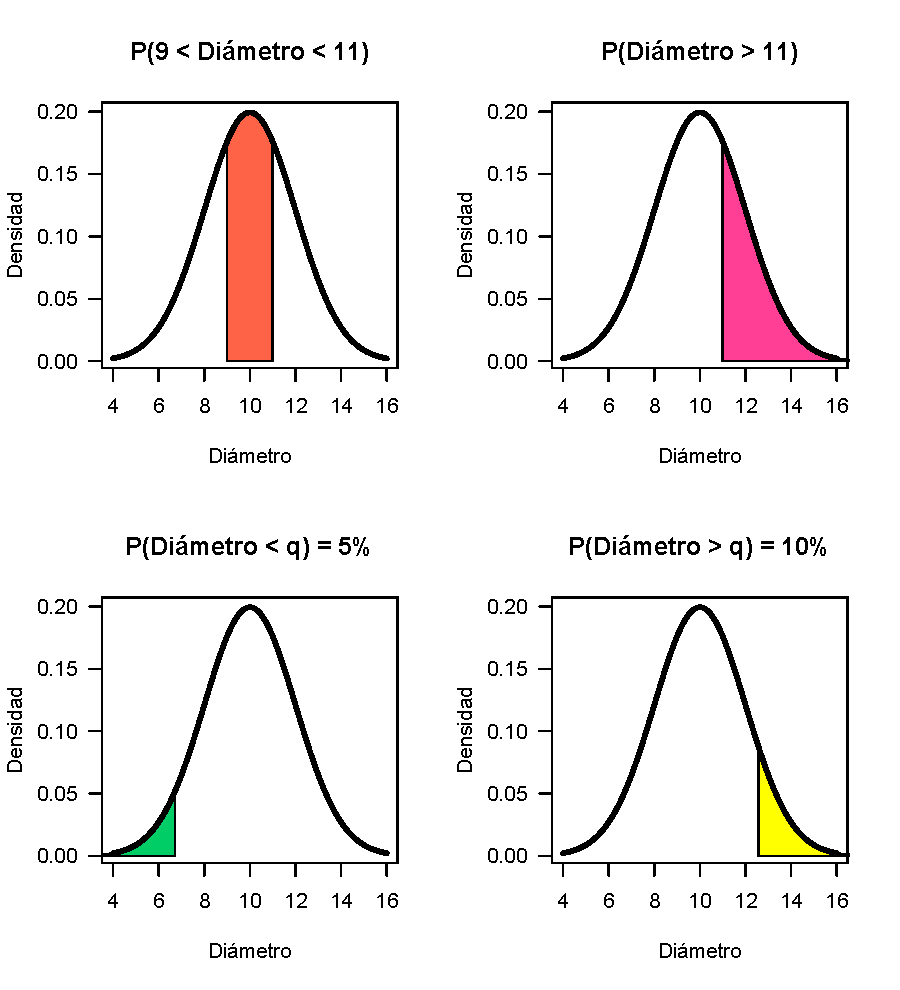
\includegraphics{Manual_de_R_files/figure-latex/norm2-1.pdf}
\caption{\label{fig:norm2}Área sombreada para el ejemplo de los tornillos.}
\end{figure}

\section{Distribuciones continuas
generales}\label{distribuciones-continuas-generales}

En la práctica nos podemos encontramos con variables aleatorias
continuas que no se ajustan a una de las distribuciones mostradas
anteriormente, en esos casos, es posible manejar ese tipo de variables
por medio de unas funciones básicas de \proglang{R} como se muestra en
el siguiente ejemplo.

\subsection*{Ejemplo}\label{ejemplo-43}


En este ejemplo se retomará la base de datos \texttt{crab} sobre el
cangrejo de herradura hembra presentado en el capítulo anterior. La base
de datos \texttt{crab} contiene las siguientes variables: el color del
caparazón, la condición de la espina, el peso en kilogramos, el ancho
del caparazón en centímetros y el número de satélites o machos sobre el
caparazón, la base de datos está disponible en el siguiente
\href{https://raw.githubusercontent.com/fhernanb/datos/master/crab}{enlace}.

\begin{enumerate}
\def\labelenumi{\arabic{enumi})}
\tightlist
\item
  Sea \(X\) la variable peso del cangrejo, dibuje la densidad para
  \(X\).
\end{enumerate}

Para obtener la densidad muestral de un vector cuantitativo se usa la
función \texttt{density}, y para dibujar la densidad se usa la función
\texttt{plot} aplicada a un objeto obtenido con \texttt{density}, a
continuación el código necesario para dibujar la densidad.

\begin{Shaded}
\begin{Highlighting}[]
\NormalTok{url <-}\StringTok{ 'https://raw.githubusercontent.com/fhernanb/datos/master/crab'}
\NormalTok{crab <-}\StringTok{ }\KeywordTok{read.table}\NormalTok{(}\DataTypeTok{file=}\NormalTok{url, }\DataTypeTok{header=}\NormalTok{T)}

\KeywordTok{plot}\NormalTok{(}\KeywordTok{density}\NormalTok{(crab$W), }\DataTypeTok{main=}\StringTok{''}\NormalTok{, }\DataTypeTok{lwd=}\DecValTok{5}\NormalTok{, }\DataTypeTok{las=}\DecValTok{1}\NormalTok{,}
     \DataTypeTok{xlab=}\StringTok{'Peso (Kg)'}\NormalTok{, }\DataTypeTok{ylab=}\StringTok{'Densidad'}\NormalTok{)}
\end{Highlighting}
\end{Shaded}

\begin{figure}[htbp]
\centering
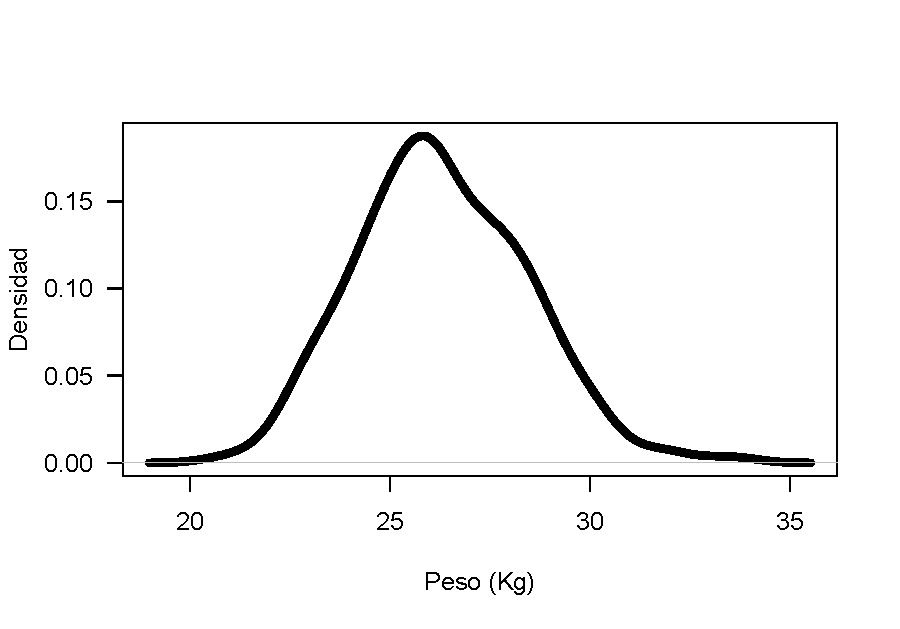
\includegraphics{Manual_de_R_files/figure-latex/crabcont1-1.pdf}
\caption{\label{fig:crabcont1}Función de densidad \(f(x)\) para el peso de
los cangrejos.}
\end{figure}

En la Figura \ref{fig:crabcont1} se muestra la densidad para la variable
peso de los cangrejos, esta densidad es bastante simétrica y el
intervalo de mayor densidad está entre 22 y 30 kilogramos.

\begin{enumerate}
\def\labelenumi{\arabic{enumi})}
\setcounter{enumi}{1}
\tightlist
\item
  Dibujar \(F(x)\) para el peso del cangrejo.
\end{enumerate}

Para dibujar la función \(F(x)\) se usa la función \texttt{ecdf} y se
almacena el resultado en el objeto \texttt{F}, luego se dibuja la
función deseada usando \texttt{plot}. A continuación el código
utilizado. En la Figura \ref{fig:crabcont2} se presenta el dibujo para
\(F(x)\).

\begin{Shaded}
\begin{Highlighting}[]
\NormalTok{F <-}\StringTok{ }\KeywordTok{ecdf}\NormalTok{(crab$W)}
\KeywordTok{plot}\NormalTok{(F, }\DataTypeTok{main=}\StringTok{''}\NormalTok{, }\DataTypeTok{xlab=}\StringTok{'Peso (Kg)'}\NormalTok{, }\DataTypeTok{ylab=}\StringTok{'F(x)'}\NormalTok{, }\DataTypeTok{cex=}\FloatTok{0.5}\NormalTok{, }\DataTypeTok{las=}\DecValTok{1}\NormalTok{)}
\end{Highlighting}
\end{Shaded}

\begin{figure}[htbp]
\centering
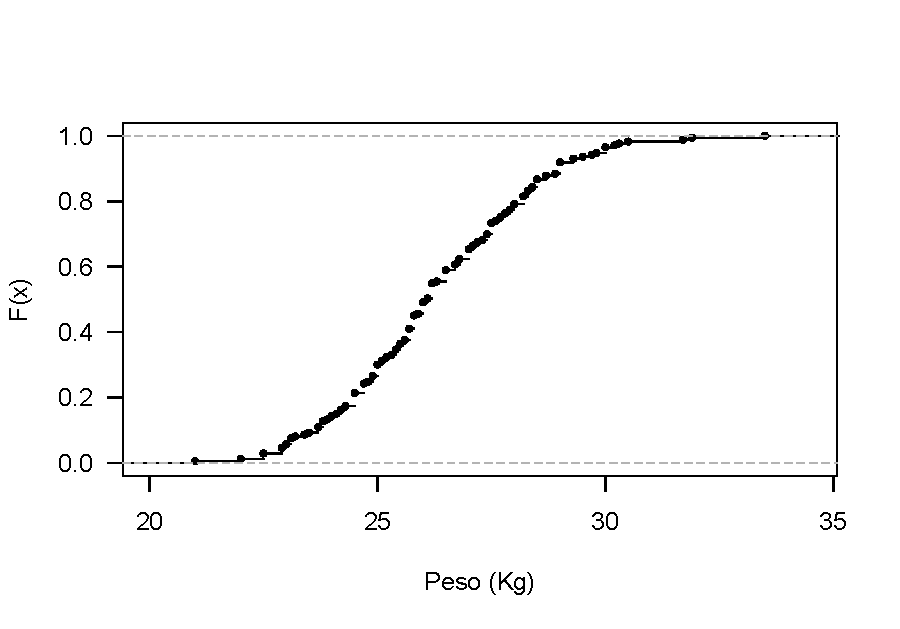
\includegraphics{Manual_de_R_files/figure-latex/crabcont2-1.pdf}
\caption{\label{fig:crabcont2}Función acumulada \(F(x)\) para el peso de los
cangrejos.}
\end{figure}

\begin{enumerate}
\def\labelenumi{\arabic{enumi})}
\setcounter{enumi}{2}
\tightlist
\item
  Calcular la probabilidad de que un cangrejo hembra tenga un peso
  inferior o igual a 28 kilogramos.
\end{enumerate}

Para obtener \(P(X \leq 28)\) se evalua en la función \(F(x)\) el
cuantil 28 así.

\begin{Shaded}
\begin{Highlighting}[]
\KeywordTok{F}\NormalTok{(}\DecValTok{28}\NormalTok{)}
\end{Highlighting}
\end{Shaded}

\begin{verbatim}
## [1] 0.7919
\end{verbatim}

Por lo tanto \(P(X \leq 28)=0.7919\).

\begin{enumerate}
\def\labelenumi{\arabic{enumi})}
\setcounter{enumi}{3}
\tightlist
\item
  Dibujar la función de densidad para el peso de los cangrejos hembra
  diferenciando por el color del caparazón.
\end{enumerate}

Como son 4 los colores de los caparazones se deben construir 4 funciones
de densidad. Usando la función \texttt{split} se puede partir el vector
de peso de los cangrejos según su color. Luego se construyen las cuatro
densidades usando la función \texttt{density} aplicada a cada uno de los
pesos, a continuación el código.

\begin{Shaded}
\begin{Highlighting}[]
\NormalTok{pesos <-}\StringTok{ }\KeywordTok{split}\NormalTok{(}\DataTypeTok{x=}\NormalTok{crab$W, }\DataTypeTok{f=}\NormalTok{crab$C)}
\NormalTok{f1 <-}\StringTok{ }\KeywordTok{density}\NormalTok{(pesos[[}\DecValTok{1}\NormalTok{]])}
\NormalTok{f2 <-}\StringTok{ }\KeywordTok{density}\NormalTok{(pesos[[}\DecValTok{2}\NormalTok{]])}
\NormalTok{f3 <-}\StringTok{ }\KeywordTok{density}\NormalTok{(pesos[[}\DecValTok{3}\NormalTok{]])}
\NormalTok{f4 <-}\StringTok{ }\KeywordTok{density}\NormalTok{(pesos[[}\DecValTok{4}\NormalTok{]])}
\end{Highlighting}
\end{Shaded}

Luego de tener las densidades muestrales se procede a dibujar la primera
densidad con \texttt{plot}, luego se usa la funció \texttt{lines} para
agregar a la densidad inicial las restantes densidades. En la Figura
\ref{fig:crabcont3} se muestran las 4 densidades, una por cada color de
caparazón.

\begin{Shaded}
\begin{Highlighting}[]
\KeywordTok{plot}\NormalTok{(f1, }\DataTypeTok{main=}\StringTok{''}\NormalTok{, }\DataTypeTok{las=}\DecValTok{1}\NormalTok{, }\DataTypeTok{lwd=}\DecValTok{4}\NormalTok{,}
     \DataTypeTok{xlim=}\KeywordTok{c}\NormalTok{(}\DecValTok{18}\NormalTok{, }\DecValTok{34}\NormalTok{),}
     \DataTypeTok{xlab=}\StringTok{'Peso (Kg)'}\NormalTok{, }\DataTypeTok{ylab=}\StringTok{'Densidad'}\NormalTok{)}
\KeywordTok{lines}\NormalTok{(f2, }\DataTypeTok{lwd=}\DecValTok{4}\NormalTok{, }\DataTypeTok{col=}\StringTok{'red'}\NormalTok{)}
\KeywordTok{lines}\NormalTok{(f3, }\DataTypeTok{lwd=}\DecValTok{4}\NormalTok{, }\DataTypeTok{col=}\StringTok{'blue'}\NormalTok{)}
\KeywordTok{lines}\NormalTok{(f4, }\DataTypeTok{lwd=}\DecValTok{4}\NormalTok{, }\DataTypeTok{col=}\StringTok{'orange'}\NormalTok{)}
\KeywordTok{legend}\NormalTok{(}\StringTok{'topright'}\NormalTok{, }\DataTypeTok{lwd=}\DecValTok{4}\NormalTok{, }\DataTypeTok{bty=}\StringTok{'n'}\NormalTok{,}
       \DataTypeTok{col=}\KeywordTok{c}\NormalTok{(}\StringTok{'black'}\NormalTok{, }\StringTok{'red'}\NormalTok{, }\StringTok{'blue'}\NormalTok{, }\StringTok{'orange'}\NormalTok{),}
       \DataTypeTok{legend=}\KeywordTok{c}\NormalTok{(}\StringTok{'Color 1'}\NormalTok{, }\StringTok{'Color 2'}\NormalTok{, }\StringTok{'Color 3'}\NormalTok{, }\StringTok{'Color 4'}\NormalTok{))}
\end{Highlighting}
\end{Shaded}

\begin{figure}[htbp]
\centering
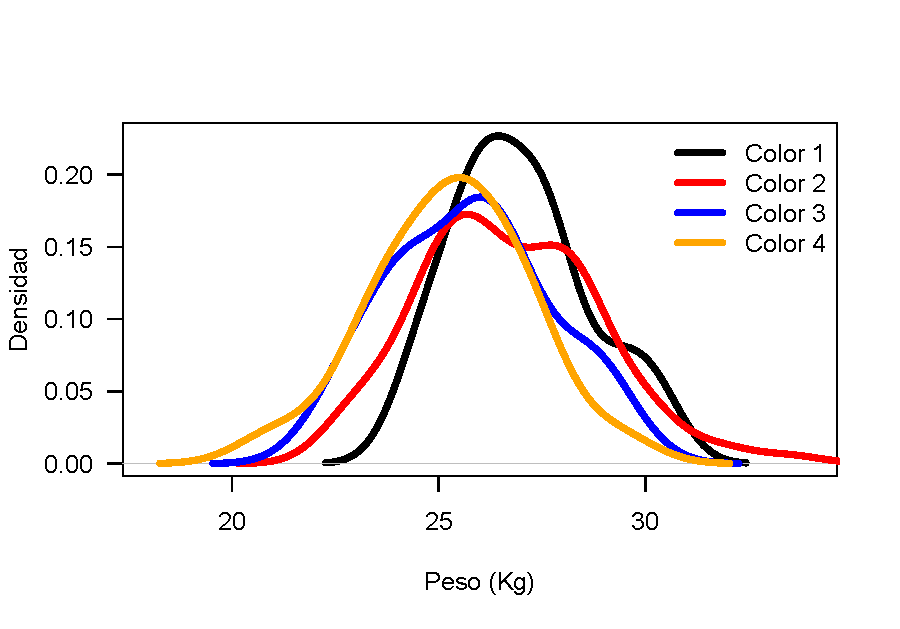
\includegraphics{Manual_de_R_files/figure-latex/crabcont3-1.pdf}
\caption{\label{fig:crabcont3}Función de densidad \(f(x)\) para el peso del
cangrejo diferenciando por el color.}
\end{figure}

Otra forma para dibujar las densidades es usar el paquete
\textbf{ggplot2} \citep{R-ggplot2}. En la Figura \ref{fig:crabcont4} se
muestra el resultado obtenido de correr el siguiente código.

\begin{Shaded}
\begin{Highlighting}[]
\KeywordTok{require}\NormalTok{(ggplot2)  }\CommentTok{# Recuerde que primero debe instalarlo}

\NormalTok{crab$Color <-}\StringTok{ }\KeywordTok{as.factor}\NormalTok{(crab$C)  }\CommentTok{# Para convertir en factor}

\KeywordTok{ggplot}\NormalTok{(crab, }\KeywordTok{aes}\NormalTok{(}\DataTypeTok{x=}\NormalTok{W)) +}\StringTok{ }
\StringTok{  }\KeywordTok{geom_density}\NormalTok{(}\KeywordTok{aes}\NormalTok{(}\DataTypeTok{group=}\NormalTok{Color, }\DataTypeTok{fill=}\NormalTok{Color), }\DataTypeTok{alpha=}\FloatTok{0.3}\NormalTok{) +}
\StringTok{  }\KeywordTok{xlim}\NormalTok{(}\DecValTok{18}\NormalTok{, }\DecValTok{34}\NormalTok{) +}\StringTok{ }\KeywordTok{xlab}\NormalTok{(}\StringTok{"Peso (Kg)"}\NormalTok{) +}\StringTok{ }\KeywordTok{ylab}\NormalTok{(}\StringTok{"Densidad"}\NormalTok{)}
\end{Highlighting}
\end{Shaded}

\begin{figure}[htbp]
\centering
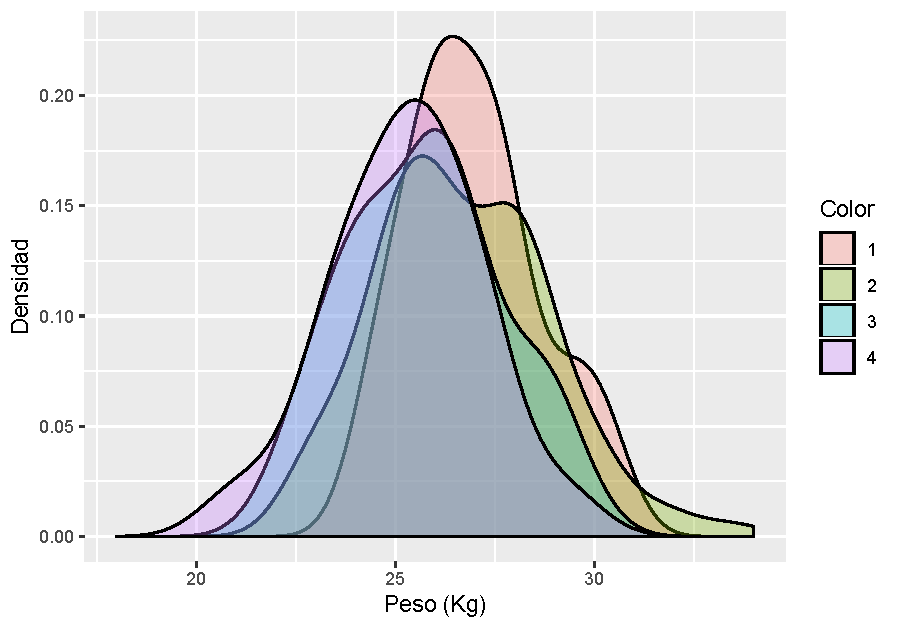
\includegraphics{Manual_de_R_files/figure-latex/crabcont4-1.pdf}
\caption{\label{fig:crabcont4}Función de densidad \(f(x)\) para el peso del
cangrejo diferenciando por el color y usando ggplot2.}
\end{figure}

Para aprender más sobre el paquete \textbf{ggplot2} se recomienda
consultar este
\href{http://tutorials.iq.harvard.edu/R/Rgraphics/Rgraphics.html}{enlace}.

\chapter{Pruebas de bondad de ajuste}\label{pruebas-de-bondad-de-ajuste}

En este capítulo se

\chapter{Aproximación de integrales}\label{aproximacion-de-integrales}

En este capítulo se mostrará cómo aproximar integrales en una y varias
dimensiones.

\section{Aproximación de Laplace
unidimensional}\label{aproximacion-de-laplace-unidimensional}

Esta aproximación es útil para obtener el valor de una integral usando
la expansión de Taylor para una función \(f(x)\) unimodal en \(\Re\), en
otras palabras lo que interesa es:
\[ I = \int_{-\infty}^{\infty} f(x) d(x)\] Al hacer una expansión de
Taylor de segundo orden para \(\log(f(x))\) en su moda \(x_0\) el
resultado es:
\[ \log(f(x)) \approx \log(f(x_0)) + \frac{\log(f)^\prime(x_0)}{1!} (x-x_0) + \frac{\log(f)^{\prime \prime}(x_0)}{2!} (x-x_0)^2 \]
El segundo término de la suma se anula porque \(\log(f)^\prime(x_0)=0\)
por ser \(x_0\) el valor donde está el máximo de \(\log(f(x))\). La
expresión anterior se simplifica en:
\[ \log(f(x)) \approx \log(f(x_0)) + \frac{\log(f)^{\prime \prime}(x_0)}{2!} (x-x_0)^2 \]
al aislar \(f(x)\) se tiene que

\begin{equation} \label{fx}
f(x) \approx f(x_0)  \exp \left( -\frac{c}{2} (x-x_0)^2 \right)
\end{equation}

donde \(c=-\frac{d^2}{dx^2} \log(f(x)) \bigg|_{x=x_0}\).

La expresión \ref{fx} se puede reescribir de manera que aparezca el
núcleo de la función de densidad de la distribución normal con media
\(x_0\) y varianza \(1/c\), a continuación la expresión

\[
f(x) \approx f(x_0) \frac{\sqrt{2 \pi / c}}{\sqrt{2 \pi / c}}  \exp \left( -\frac{1}{2} \left( \frac{x-x_0}{1/\sqrt{c}} \right)^2 \right)
\] Así al calcular la integral de \(f(x)\) en \(\Re\) se tiene que:

\begin{equation} \label{aprox_laplace}
I = \int_{-\infty}^{\infty} f(x) d(x) = f(x_0) \sqrt{2 \pi / c}
\end{equation}

\subsection*{Ejemplo}\label{ejemplo-44}


Calcular la integral de \(f(x)=\exp \left( -(x-1.5)^2 \right)\) en
\(\Re\) utilizando la aproximación de Laplace.

Primero vamos a dibujar la función \(f(x)\) para ver en dónde está su
moda \(x_0\).

\begin{Shaded}
\begin{Highlighting}[]
\NormalTok{fun <-}\StringTok{ }\NormalTok{function(x) }\KeywordTok{exp}\NormalTok{(-(x}\FloatTok{-1.5}\NormalTok{)^}\DecValTok{2}\NormalTok{)}
\KeywordTok{curve}\NormalTok{(fun, }\DataTypeTok{from=}\NormalTok{-}\DecValTok{5}\NormalTok{, }\DataTypeTok{to=}\DecValTok{5}\NormalTok{, }\DataTypeTok{ylab=}\StringTok{'f(x)'}\NormalTok{, }\DataTypeTok{las=}\DecValTok{1}\NormalTok{)}
\end{Highlighting}
\end{Shaded}

\begin{figure}[htbp]
\centering
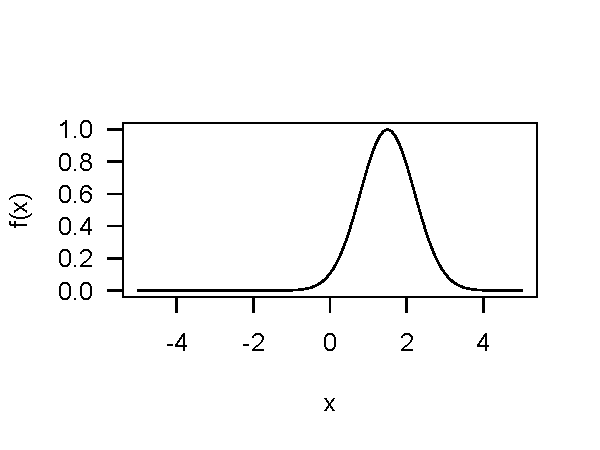
\includegraphics{Manual_de_R_files/figure-latex/unnamed-chunk-213-1.pdf}
\caption{\label{fig:unnamed-chunk-213}Perfil de la función f(x).}
\end{figure}

Visualmente se nota que la moda está cerca del valor 1.5 y para
determinar numéricamente el valor de la moda \(x_0\) se usa la función
\texttt{optimize}, los resultados se almacenan en el objeto
\texttt{res}. El valor de la moda corresponde al elemento
\texttt{maximum} del objeto \texttt{res}.

\begin{Shaded}
\begin{Highlighting}[]
\NormalTok{res <-}\StringTok{ }\KeywordTok{optimize}\NormalTok{(fun, }\DataTypeTok{interval=}\KeywordTok{c}\NormalTok{(-}\DecValTok{10}\NormalTok{, }\DecValTok{10}\NormalTok{), }\DataTypeTok{maximum=}\OtherTok{TRUE}\NormalTok{)}
\NormalTok{res}
\end{Highlighting}
\end{Shaded}

\begin{verbatim}
## $maximum
## [1] 1.5
## 
## $objective
## [1] 1
\end{verbatim}

Para determinar el valor de \(c\) de la expresión \ref{aprox_laplace} se
utiliza el siguiente código.

\begin{Shaded}
\begin{Highlighting}[]
\KeywordTok{require}\NormalTok{(}\StringTok{"numDeriv"}\NormalTok{)}
\NormalTok{constant <-}\StringTok{ }\NormalTok{-}\StringTok{ }\KeywordTok{as.numeric}\NormalTok{(}\KeywordTok{hessian}\NormalTok{(fun, res$maximum))}
\end{Highlighting}
\end{Shaded}

Para obtener la aproximación de la integral se usa la expresión
\ref{aprox_laplace} y para tener un punto de comparación se evalua la
integral usando la función \texttt{integrate}, a continuación el código.

\begin{Shaded}
\begin{Highlighting}[]
\KeywordTok{fun}\NormalTok{(res$maximum) *}\StringTok{ }\KeywordTok{sqrt}\NormalTok{(}\DecValTok{2}\NormalTok{*pi/constant)}
\end{Highlighting}
\end{Shaded}

\begin{verbatim}
## [1] 1.772
\end{verbatim}

\begin{Shaded}
\begin{Highlighting}[]
\KeywordTok{integrate}\NormalTok{(fun, -}\OtherTok{Inf}\NormalTok{, }\OtherTok{Inf}\NormalTok{)  }\CommentTok{# Para comparar}
\end{Highlighting}
\end{Shaded}

\begin{verbatim}
## 1.772 with absolute error < 1.5e-06
\end{verbatim}

De los anteriores resultados vemos que la aproximación es buena.

\bibliography{packages,book}

\backmatter
\printindex

\end{document}
